% !TEX TS-program = latex
% !TEX spellcheck = it-IT
\documentclass[a4paper]{article}
\usepackage[utf8]{inputenc}
\usepackage[T1]{fontenc}
\usepackage[italian]{babel}
\usepackage{tikz} % LATEX
\usetikzlibrary {automata}


%%%%%%%%%%%%%%%%%%%%%%%%%%%%%%%%%%%%%%%%%%%%%%%%%%%%%%%%%%%%%%%%%%%%%%%%%%%%
%% Trim Size: 9.75in x 6.5in
%% Text Area: 8in (include Runningheads) x 5in
%% ws-ijgmmp.tex   :   2-9-08
%% Tex file to use with ws-ijgmmp.cls written in Latex2E.
%% The content, structure, format and layout of this style file is the
%% property of World Scientific Publishing Co. Pte. Ltd.
%% Copyright 1995, 2002 by World Scientific Publishing Co.
%% All rights are reserved.
%%%%%%%%%%%%%%%%%%%%%%%%%%%%%%%%%%%%%%%%%%%%%%%%%%%%%%%%%%%%%%%%%%%%%%%%%%%%
%%

%%%%%%%%%%%%%%%%%%%%%%%%%%%%%


\usepackage{pictexwd,dcpic}
\usepackage{csquotes}
\usepackage{nopageno}

\usepackage{amsmath, amssymb, amsthm}
\usepackage{pictex, dcpic}
\usepackage{color}
%\usepackage{graphicx}
%\numberwithin{equation}{section} % This line resets equation numbering when starting a new section.
%\renewcommand{\theequation}{Eq. \thesection.\arabic{equation}} % This line ads "Eq." in front of your equation numbering.
\usepackage{hyperref}


\def\http#1#2{\href{#1}{#2}}



%
%    Macros.    Version 1.2.0.beta
%    The best use is to paste all of them into the papers
%     1/8/2005
%

%%%%%%%%%%%%%%%%%%%%%%%%%%%%%%
%%%%%%			Greek		 %%%%%%
%%%%%%%%%%%%%%%%%%%%%%%%%%%%%%

\def\al{\alpha}
\def\be{\beta}
\def\de{\delta}
\def\ga{\gamma}
\def\up{\upsilon}
\def\ep{\epsilon}
\def\io{\iota}
\def\te{\theta}
\def\la{\lambda}
\def\ze{\zeta}
\def\om{\omega}
\def\si{\sigma}
\def\vp{\varphi}
\def\vpi{\varpi}
\def\ka{\kappa}
\def\vs{\varsigma}
\def\vr{\varrho}

\def\De{\Delta}
\def\Ga{\Gamma}
\def\Te{\Theta}
\def\La{\Lambda}
\def\Om{\Omega}
\def\Si{\Sigma}
\def\Up{\Upsilon}

\def\boldDe{\bf\Delta}
\def\boldGa{\bf\Gamma}
\def\boldTe{\bf\Theta}
\def\boldLa{\bf\Lambda}
\def\boldOm{\bf\Omega}
\def\boldSi{\bf\Sigma}
\def\boldUp{\bf\Upsilon}
\def\boldXi{\bf\Xi}
\def\boldPi{\bf\Pi}
\def\boldPhi{\bf\Phi}
\def\boldPsi{\bf\Psi}

\def\boldal{\bf\al}
\def\boldbe{\bf\be}
\def\boldga{\bf\ga}
\def\boldde{\bf\de}
\def\boldep{\bf\ep}
\def\boldze{\bf\ze}
\def\boldeta{\bf\eta}
\def\boldte{\bf\te}
\def\boldio{\bf\io}
\def\boldka{\bf\ka}
\def\boldla{\bf\la}
\def\boldmu{\hbox{\greekbold\char "16}}
\def\boldnu{\hbox{\greekbold\char "17}}
\def\boldxi{\hbox{\greekbold\char "18}}
\def\boldpi{\hbox{\greekbold\char "19}}
\def\boldrho{\hbox{\greekbold\char "1A}}
\def\boldsi{\bf\si}
\def\boldtau{\hbox{\greekbold\char "1C}}
\def\boldup{\hbox{\greekbold\char "1D}}
\def\boldphi{\hbox{\greekbold\char "1E}}
\def\boldchi{\hbox{\greekbold\char "1F}}
\def\boldpsi{\hbox{\greekbold\char "20}}
\def\boldom{\hbox{\greekbold\char "21}}
\def\boldvep{\hbox{\greekbold\char "22}}
\def\boldvte{\hbox{\greekbold\char "23}}
\def\boldvpi{\hbox{\greekbold\char "24}}
\def\boldvrho{\hbox{\greekbold\char "25}}
\def\boldvsi{\hbox{\greekbold\char "26}}
\def\boldvphi{\hbox{\greekbold\char "27}}

%%%%%%%%%%%%%%%%%%%%%%%%%%%%%%
%%%%%%			Cal			 %%%%%%
%%%%%%%%%%%%%%%%%%%%%%%%%%%%%%
 \def\calA{{\hbox{\cal A}}}
 \def\calU{{\hbox{\cal U}}}
 \def\calB{{\hbox{\cal B}}}
 \def\calC{{\hbox{\cal C}}}
 \def\calI{{\hbox{\cal I}}}
 \def\Card{{\hbox{Card}}}
 \def\calQ{{\hbox{\cal Q}}}
 \def\calP{{\hbox{\cal P}}}
 \def\calL{{\hbox{\cal L}}}
 \def\calE{{\hbox{\cal E}}}
 \def\calW{{\hbox{\cal W}}}
 \def\calV{{\hbox{\cal V}}}
 \def\calS{{\hbox{\cal S}}}
 \def\calF{{\hbox{\cal F}}}
 \def\calR{{\hbox{\cal R}}}
 \def\calO{{\hbox{\cal O}}}
 \def\calM{{\hbox{\cal M}}}

%%%%%%%%%%%%%%%%%%%%%%%%%%%%%%
%%%%%%			gothic		 %%%%%%
%%%%%%%%%%%%%%%%%%%%%%%%%%%%%%
 \def\su{{\mathfrak{su}}}
 \def\gl{{\mathfrak{gl}}}
 \def\gotg{{\mathfrak{g}}}
 \def\goth{{\mathfrak{h}}}
 \def\gotm{{\mathfrak{m}}}
 \def\gotk{{\mathfrak{k}}}
 \def\spin{{\mathfrak{spin}}}
 \def\slC{{\mathfrak{sl}}}
 \def\O{{\mathfrak{O}}}
 \def\Set{{\mathfrak{Set}}}

%%%%%%%%%%%%%%%%%%%%%%%%%%%%%%
%%%%%%			Bbb			 %%%%%%
%%%%%%%%%%%%%%%%%%%%%%%%%%%%%%
 \def\one{\mathbb{I}}
 \def\A{\mathbb{A}}
 \def\B{\mathbb{B}}
 \def\C{\mathbb{C}}
 \def\D{\mathbb{D}}
 \def\E{\mathbb{E}}
 \def\F{\mathbb{F}}
 \def\G{\mathbb{G}}
 \def\H{\mathbb{H}}
 \def\J{\mathbb{J}}
 \def\K{\mathbb{K}}
 \def\I{\mathbb{I}}
 \def\L{\mathbb{L}}
 \def\M{\mathbb{M}}
 \def\N{\mathbb{N}}
 \def\O{\mathbb{O}}
 \def\P{\mathbb{P}}
 \def\Q{\mathbb{Q}}
 \def\R{\mathbb{R}}
 \def\S{\mathbb{S}}
 \def\T{\mathbb{T}}
 \def\U{\mathbb{U}}
 \def\V{\mathbb{V}}
 \def\X{\mathbb{X}}
 \def\Y{\mathbb{Y}}
 \def\W{\mathbb{W}}
 \def\Z{\mathbb{Z}}
 

%%%%%%%%%%%%%%%%%%%%%%%%%%%%%%
%%%%%%		MathRoman		 %%%%%%
%%%%%%%%%%%%%%%%%%%%%%%%%%%%%%
\def\Tr{{\hbox{Tr}}}
\def\Con{{\hbox{Con}}}
\def\Aut{{\hbox{Aut}}}
\def\Div{{\hbox{Div}}}
\def\ad{{\hbox{ad}}}
\def\Ad{{\hbox{Ad}}}
\def\Re{{\hbox{Re}}}
\def\Im{{\hbox{Im}}}
\def\Iso{{\hbox{Iso}}}
\def\Geo{{\hbox{Geo}}}
\def\Int{{\hbox{Int}}}
\def\Inv{{\hbox{Inv}}}
\def\Spin{{\hbox{Spin}}}
\def\SO{{\hbox{SO}}}
\def\SU{{\hbox{SU}}}
\def\SL{{\hbox{SL}}}
\def\GL{{\hbox{GL}}}
\def\det{{\hbox{det}}}
\def\Hom{{\hbox{Hom}}}
\def\End{{\hbox{End}}}
\def\Euc{{\hbox{Euc}}}
\def\Lor{{\hbox{Lor}}}
\def\Diff{{\hbox{Diff}}}
\def\di{{\hbox{d}}}
\def\id{{\hbox{\rm id}}}
\def\diag{{\hbox{diag}}}
\def\rank{{\hbox{rank}}}
\def\span{{\hbox{span}}}
\def\Sim{{\hbox{Sim}}}

\def\Obj{{\hbox{Obj}}}

%%%%%%%%%%%%%%%%%%%%%%%%%%%%%%
%%%%%%		OtherSymbols		 %%%%%%
%%%%%%%%%%%%%%%%%%%%%%%%%%%%%%
\def\ip{\hbox to4pt{\leaders\hrule height0.3pt\hfill}\vbox to8pt{\leaders\vrule width0.3pt\vfill}\kern 2pt}

% inner product
\def\QDE{\hfill\hbox{\ }\vrule height4pt width4pt depth0pt} 
\def\del{\partial}
\def\na{\nabla}
\def\inter{\cap}
\def\Vec{\mathfrak{X}}
\def\Lie{\hbox{\LieFont \$}}

\def\arr{\rightarrow}
\def\larr{\longrightarrow}
\def\harr{\hookrightarrow}
\def\hlarr{\lhook\joinrel\longrightarrow}
\def\then{\Rightarrow}
\def\semidirect{\hbox{\Bbb \char111}}
\def\binomial#1#2{\left(\Matrix{#1\cr #2\cr}\right)}

\def\barJ{\bar J}

\def\sSU{{\hbox{SU}}}
\def\so{{so}}
%\def\N{{{\mathbb N}}}

\def\file#1{{\tt #1}}
\def\calH{{{\cal H}}}
\def\calJ{{{\cal J}}}
\def\calG{{{\cal G}}}
\def\calK{{{\cal K}}}
\def\calD{{{\cal D}}}
\def\scalD{{{\cal D}}}

\def\Loop{{\hbox{Loop}}}
\def\Hoop{{\hbox{Hoop}}}
\def\Sym{{\hbox{Sym}}}
\def\sR{{\R}}
\def\dCor{dCor}
\def\epm{\hbox{$^\pm$}}
\def\dunion{\coprod}

\def\nab#1{{\buildrel #1\over \na}}
\def\frac[#1/#2]{\hbox{$#1\over#2$}}
\def\Frac[#1/#2]{{#1\over#2}}
\def\({\left(}
\def\){\right)}
\def\[{\left[}
\def\]{\right]}
\def\^#1{{}^{#1}_{\>\cdot}}
\def\_#1{{}_{#1}^{\>\cdot}}
\def\Label=#1{{\buildrel {\hbox{\fiveSerif \ShowLabel{#1}}}\over =}}
\def\<{\kern -1pt}
\def\Bar{\>|\>}
\def\Dal{\hbox{\tenRelazioni  \char003}}

\def\uvec#1{\vbox{\hbox{$\scriptstyle\rightharpoonup$}\vskip-9pt\hbox{$#1$}}}
\def\dvec#1{\vtop{\hbox{$#1$}\vskip-10pt\hbox{$\scriptstyle\rightharpoondown$}}}
\def\Cprod{\diamond}
\def\obullet{\odot}
\def\cbrt{{}^3\kern-5pt\sqrt}



%%%%%%%%%%%%			frames 				%%%%%%%%%%%%%%%%%%%

\def\red#1{{\color{red}{#1}}}
\def\blue#1{{\color{blue}{#1}}}
\def\green#1{{\color{green}{#1}}}

\def\Red{\color{red}}
\def\Blue{\color{blue}}
\def\Green{\color{green}}


\def\frame#1{\vbox{\hrule\hbox{\vrule\vbox{\kern2pt\hbox{\kern2pt#1\kern2pt}\kern2pt}\vrule}\hrule\kern-4pt}} 
\def\redframe#1{\red{\frame{#1}}} 
\def\greenframe#1{\green{\frame{#1}}} 
\def\blueframe#1{\blue{\frame{#1}}} 

\def\uline#1{\underline{#1}}
\def\uuline#1{\underline{\underline{#1}}}
\def\Box to #1#2#3{\frame{\vtop{\hbox to #1{\hfill #2 \hfill}\hbox to #1{\hfill #3 \hfill}}}}



\def\ubal{\underline{\al}\kern1pt}
\def\obal{\overline{\al}\kern1pt}

\def\ubR{\underline{R}\kern1pt}
\def\obR{\overline{R}\kern1pt}
\def\ubom{\underline{\om}\kern1pt}
\def\obxi{\overline{\xi}\kern1pt}
\def\ubu{\underline{u}\kern1pt}
\def\ube{\underline{e}\kern1pt}
\def\obe{\overline{e}\kern1pt}
\def\Limit{\>{\buildrel{r\arr\infty}\over \longrightarrow}\,}
\def\union{\cup}
\def\Emptyset{\varnothing}




\def\Uvec#1{\vbox{\mathsurround=0pt\ialign{##\crcr
     $\scriptscriptstyle\rightharpoonup$\crcr\noalign{\kern1pt\nointerlineskip}
     $\hfil\displaystyle{#1}\hfil$\crcr}}}
\def\Dvec#1{\vbox{\mathsurround=0pt\ialign{##\crcr
     $\scriptscriptstyle\rightharpoondown$\crcr\noalign{\kern-7pt\nointerlineskip}
     $\hfil\displaystyle{#1}\hfil$\crcr}}}


%   u 
\def\uvecu{\vbox{\mathsurround=0pt\ialign{##\crcr
     $\scriptscriptstyle\rightharpoonup$\crcr\noalign{\kern1pt\nointerlineskip}
     $\hfil\displaystyle{u}\hfil$\crcr}}}
\def\dvecu{\vbox{\mathsurround=0pt\ialign{##\crcr
     $\scriptscriptstyle\rightharpoondown$\crcr\noalign{\kern-7pt\nointerlineskip}
     $\hfil\displaystyle{u}\hfil$\crcr}}}
%\def\uvecu{\Uvec{u}}
%\def\dvecu{\Dvec{u}}

%   be
\def\uvecbe{\vbox{\mathsurround=0pt\ialign{##\crcr
     \kern3pt$\scriptscriptstyle\rightharpoonup$\crcr\noalign{\kern1pt\nointerlineskip}
     $\hfil\displaystyle{\be}\hfil$\crcr}}}
\def\dvecbe{\vbox{\mathsurround=0pt\ialign{##\crcr
     \kern1pt$\scriptscriptstyle\rightharpoondown$\crcr\noalign{\kern-10pt\nointerlineskip}
     $\hfil\displaystyle{\be}\hfil$\crcr}}}

%   n
\def\uvecn{\vbox{\mathsurround=0pt\ialign{##\crcr
     $\scriptscriptstyle\rightharpoonup$\crcr\noalign{\kern1pt\nointerlineskip}
     $\hfil\displaystyle{n}\hfil$\crcr}}}
\def\dvecn{\vbox{\mathsurround=0pt\ialign{##\crcr
     $\scriptscriptstyle\rightharpoondown$\crcr\noalign{\kern-7pt\nointerlineskip}
     $\hfil\displaystyle{n}\hfil$\crcr}}}

%   m
\def\uvecm{\vbox{\mathsurround=0pt\ialign{##\crcr
     $\scriptscriptstyle\rightharpoonup$\crcr\noalign{\kern1pt\nointerlineskip}
     $\hfil\displaystyle{m}\hfil$\crcr}}}
\def\dvecm{\vbox{\mathsurround=0pt\ialign{##\crcr
     $\scriptscriptstyle\rightharpoondown$\crcr\noalign{\kern-7pt\nointerlineskip}
     $\hfil\displaystyle{m}\hfil$\crcr}}}

%   N
\def\uvecN{\vbox{\mathsurround=0pt\ialign{##\crcr
     \kern3pt$\scriptscriptstyle\rightharpoonup$\crcr\noalign{\kern1pt\nointerlineskip}
     $\hfil\displaystyle{N}\hfil$\crcr}}}
\def\dvecN{\vbox{\mathsurround=0pt\ialign{##\crcr
     \kern0pt$\scriptscriptstyle\rightharpoondown$\crcr\noalign{\kern-10pt\nointerlineskip}
     $\hfil\displaystyle{N}\hfil$\crcr}}}

%   u
\def\uvecu{\vbox{\mathsurround=0pt\ialign{##\crcr
     $\scriptscriptstyle\rightharpoonup$\crcr\noalign{\kern1pt\nointerlineskip}
     $\hfil\displaystyle{u}\hfil$\crcr}}}
\def\dvecu{\vbox{\mathsurround=0pt\ialign{##\crcr
     $\scriptscriptstyle\rightharpoondown$\crcr\noalign{\kern-7pt\nointerlineskip}
     $\hfil\displaystyle{u}\hfil$\crcr}}}

%   w
\def\uvecw{\vbox{\mathsurround=0pt\ialign{##\crcr
     $\scriptscriptstyle\rightharpoonup$\crcr\noalign{\kern1pt\nointerlineskip}
     $\hfil\displaystyle{w}\hfil$\crcr}}}
\def\dvecw{\vbox{\mathsurround=0pt\ialign{##\crcr
     $\scriptscriptstyle\rightharpoondown$\crcr\noalign{\kern-7pt\nointerlineskip}
     $\hfil\displaystyle{w}\hfil$\crcr}}}

%   v
\def\uvecv{\vbox{\mathsurround=0pt\ialign{##\crcr
     $\scriptscriptstyle\rightharpoonup$\crcr\noalign{\kern1pt\nointerlineskip}
     $\hfil\displaystyle{v}\hfil$\crcr}}}
\def\dvecv{\vbox{\mathsurround=0pt\ialign{##\crcr
     $\scriptscriptstyle\rightharpoondown$\crcr\noalign{\kern-7pt\nointerlineskip}
     $\hfil\displaystyle{v}\hfil$\crcr}}}

\def\astA{{}^\ast A}
\def\circA{{}^\circ A}
\def\astk{{}^\ast k}
\def\circk{{}^\circ k}
\def\astK{{}^\ast K}
\def\circK{{}^\circ K}
\def\astL{{}^\ast L}
\def\circL{{}^\circ L}
\def\astal{{}^\ast \al}
\def\circal{{}^\circ \al}
\def\astsi{{}^\ast \si}
\def\circsi{{}^\circ \si}
\def\aste{{}^\ast e}
\def\circe{{}^\circ e}
\def\astte{{}^\ast \te}
\def\circte{{}^\circ \te}
\def\astGa{{}^\ast \Ga}
\def\circGa{{}^\circ \Ga}
\def\Lie{\pounds}

\long\def\Hide#1{}
\long\def\HideMarked#1{\hfill{$\triangleright$}}
\def\rtau{\tau}


%%%%%%%%%%%%%%%%%%%%%%%%%%%%%%%%%%%%%%%%%%%%%%%%%%%%%%%%%%%%%%%
\def\NormalStyle{\leftskip=0cm\rightskip=0cm\normalsize\parindent=5pt\parskip=3pt\normalbaselineskip=14pt\baselineskip=\normalbaselineskip}
\def\AbstractStyle{\leftskip=1cm\rightskip=1cm\scriptsize\parindent=0pt\parskip=0pt\normalbaselineskip=11pt\baselineskip=\normalbaselineskip}\def\NoteStyle{\leftskip=1cm\rightskip=1cm\scriptsize\parindent=0pt\parskip=0pt\normalbaselineskip=11pt\baselineskip=\normalbaselineskip}

\def\ShowLabel#1{\ref{#1}}

\def\Bibliography{\begin{thebibliography}{199}\footnotesize\References}
\def\EndBibliography{\end{thebibliography}}
\def\bib#1#2{\bibitem{#1}#2}
\def\Ref#1{\cite{#1}}


\def\NewSection#1{\section{#1}}
\def\NewSubSection#1{\subsection*{#1}}
\def\NewAppendix#1#2{\section*{Appendix #1: #2}}
\def\Acknowledgements{\section*{Acknowledgements}}
\def\bs{\bigskip}
\def\ms{\medskip}
\def\ss{\smallskip}
\def\ni{\noindent}

\long\def\Note#1{\blockquote{\footnotesize {\bf Nota:}~#1\par}}
\long\def\Ex#1{\blockquote{\footnotesize {\bf Esercizio:}~#1\par}}

\def\eq#1{\begin{equation}#1\end{equation}}
\def\eqLabel#1#2{\begin{equation}#1\label{#2}\end{equation}}


\def\Cases#1{\begin{cases}#1\end{cases}}
\def\Matrix#1{\begin{matrix}#1\end{matrix}}
\def\Align#1{\begin{aligned}#1\end{aligned}}

\def\eqs#1{\eq{\Align{#1}}}
\def\eqsLabel#1#2{\eq{\Align{#1}\label{#2}}}




\def\Abstract{\AbstractStyle{\bf Abstract. }}
\def\EndAbstract{\par\NormalStyle}

\def\TitleScript{}
\def\TitleLine#1{\def\TitleScript{#1}}
\def\MoreTitleLine#1{\edef\TitleScript{\TitleScript\\#1}}

\def\AuthorScript{}
\def\AuthorLine#1{\def\AuthorScript{#1}}
\def\MoreAuthorLine#1{\edef\AuthorScript{\AuthorScript\\#1}}

\def\AddressScript{}
\def\AddressLine#1{\def\AddressScript{#1}}
\def\MoreAddressLine#1{\edef\AddressScript{\AddressScript\\#1}}

\date{}

\def\BeginDocument{\begin{document}}

\def\MakeTitle{
\begin{center}
{\Large\bf\sffamily\baselineskip=2pt\TitleScript}\\
\vskip 10pt
{\small by {\it \AuthorScript}}\\
\vskip 10pt
{\small \AddressScript}
\end{center}
\ms
}

\def\EndDocument{\end{document}}

\def\Figure[#1]#2{\begin{figure}[htbp] %  figure placement: here, top, bottom, or page
   \centering
   \includegraphics[#1]{#2} }
\def\Caption#1{\caption{#1}}
\def\EndFigure{\end{figure}}

\def\Diagram#1{\eq{
\begindc{\commdiag}[10]
#1
\enddc%
}%
}

\def\Itemize#1{\begin{itemize}#1\end{itemize}}
\def\Item[#1]{\item[#1]}

\def\AllReferences{}



\def\Shrink{\small}
%%%%%%%%%%%%%%%%%%%%%%%%%%%%%%%%%%%%%%%%%%%%%%%%%
%%%%%%%%%%%%%%%%%%%%%%%%%%%%%%%%%%%%%%%%%%%%%%%%%%%

%\BeginDocument


%%%%%%%%%%%%%%%%%%%%%%%%%%%%%%%%%%%%%%%%%%%%%%%%%%%






















\parindent=5pt
\baselineskip=13pt
\parskip=5pt





\begin{document}

\AllReferences


%%%%%%%%%%%%%%%%%%%%% Publisher's Area please ignore %%%%%%%%%%%%%%%
%
%
%%%%%%%%%%%%%%%%%%%%%%%%%%%%%%%%%%%%%%%%%%%%%%%%%%%%%%%%%%%%%%%%%%%%

\title{Matematica per adulti}

\maketitle

\NewSection{Introduzione}

Tutto ciò nasce su Hookii. Un utente ha espresso il desiderio (forse buttato là) di ristudiare la matematica per vedere se era proprio vero che era incomprensibile, io (un po' per gioco) mi sono offerto di dargli una mano.

Qui di seguito le presentazioni.

\NewSubSection{Matematica per adulti:
no, non è una sezione di pornhub}



Da Wikipedia: L'UNESCO definisce dal 1984 l'analfabetismo funzionale come 

{\blockquote{\footnotesize la condizione di una persona incapace di comprendere, valutare, usare e farsi coinvolgere da testi scritti per intervenire attivamente nella società, per raggiungere i propri obiettivi e per sviluppare le proprie conoscenze e potenzialità.\par}
 
Ho cinquant’anni suonati, di cui quasi trenta passati nel mondo del lavoro della PMI veneta, sezione logistica e successivamente acquisti. 

Ho sempre avuto a che fare coi numeri, che fossero quantità o somme di denaro (nell’industria queste cose vanno spesso a braccetto), e li ho sempre usati con la consapevolezza che le quattro operazioni aritmetiche bastassero e avanzassero per gli scopi che ero tenuto a raggiungere. Ed è così! Questo la dice lunga sullo stato delle PMI venete, immagino. 

In sostanza, per quanto riesca a sostenere una conversazione coi congiuntivi senza subire vari ictus da sforzo, sono matematicamente nella stessa situazione in cui l’ingegnere dell’ufficio tecnico si trovava ogni volta che scriveva una mail o un rapporto. Ricordo che con alcuni colleghi ci si dava di gomito evidenziando gli strafalcioni e la sua incapacità di scrivere un italiano vagamente comprensibile (in una persona peraltro altamente educata nel proprio campo). 

Rispetto all’ingegnere avevo un vantaggio, sapevo che se avessi usato dei numeri oltre le quattro operazioni mi sarei esposto al ridicolo, quindi neanche ci provavo.

Poi, con circa trentacinque anni di ritardo (lo so, mi chiamano lo Svelto), l’illuminazione: io ero uguale a lui, solo non con l’italiano. In questo devo ammettere che hookii mi ha aiutato visto che almeno metà degli utenti è un luminare in qualche hard science, o magari non così hard ma di sicuro più hard di quanto io abbia mai sognato (per quelli come me che non hanno mai superato l’umorismo delle elementari, non sto parlando del mondo della pornografia). 

Anni e anni a leggere, guardare, informarmi sulla scienza e sulla tecnologia e mi sarei vergognato a dire una sola parola sull’argomento perché conoscevo solo i risultati, la divulgazione, le scoperte e così via. 

Non conoscevo il modo, non conoscevo il lavoro e soprattutto non conoscevo il linguaggio su cui si basa un’enorme parte della conoscenza umana. 

Potrei scrivere parecchio sui motivi che mi hanno reso funzionale sebbene analfabeta ma non è lo scopo di questa mia, e comunque negli anni ho realizzato di essere stato molto più colpevole che vittima. Ho sempre pensato che la natura mi abbia fornito un cervello di prim’ordine (beh?) ma in fondo al contratto era scritta una minuscola, impercettibile clausola per cui quel chiletto di materia grigia arrivava dotato di una colossale mancanza di autodisciplina. Se nessuno mi innesta con violenza un’alabarda sulle gengive, difficilmente combino qualcosa: non vi ricordo il classico asino (anche come taglio di capelli)? Però molto più bastone che carote, che tra l’altro mi fanno schifo.

Qui arriviamo a {\it Matematica per adulti}, una sezione di Hookii dedicata a chi, come me, deve imparare una lingua nuova e differente e implementare circuiti cerebrali dormienti o direttamente assenti. 

Ultime righe per ringraziare {\tt Baol}, che si è assunto l’onere di questa improba fatica (gratis, che qui non ci abbiamo i dobloni) e tutti gli altri che lo stanno aiutando a partire da {\tt ulrich}. 

Grazie anche a {\tt gsax}, che pur avendo già i suoi mostruosi problemi mentali cerca comunque di darmi una mano. È un amico, ma non si sa di chi.

Abbiate pazienza.

Dalla prossima volta “parlerò di numeri”.


\NewSubSection{Virgilio}

Visto che siamo di presentazioni, sono {\tt Baol}, sono un matematico e un fisico, ho più o meno l'età di {\tt Angvarr} e, come tutti i maghi Baol, non esisto.
Ho sempre trovato facile la matematica, non ho mai avuto un quaderno di matematica fino all'università, molto più complicata l'umanità.
In particolare non ho mai capito cosa si potesse trovare di difficile a capire la matematica, {\it ça va sans dire}.

Fatto sta che sono sempre stato un peripatetico della matematica, anche tra i matematici sono uno dei meno specializzati nel senso che ho fatto cose in tante aree che normalmente sono disconnesse. Per il ministero sono un matematico applicato ma ho sempre frequentato anche la parte più formale  e astratta della matematica.

Siccome ho una figlia {\tt Baolina} sono passato per le scuole 2 volte, una volta da studente una volta da genitore muto (perché i genitori non si devono immischiare nella vita dei figli). Baolina ha sempre avuto maestre che, a loro dire, si sentivano inadeguate a insegnare matematica alle elementari (e infatti a seguire troppo i libri ne hanno combinate delle belle).

Ho visto cose tipo usare la retta dei numeri per dare una rappresentazione di numeri naturali, parlare dei numeri amici prima di dire cosa era la somma (per {\it insegnare} a fare la somma, due numeri $a$ e $b$ sono amici del 10 se $a+b=10$, in pratica una relazione ternaria (una relazione in $(\N\times \N)\times \N$), le {\it parole chiave} per risolvere i problemi (se nel testo c'è {\it in tutto}, {\it in totale},  allora devi fare la somma).

E mi sono sempre chiesto, ma se ti senti inadeguato, non sarebbe meglio leggere un po' e farsi un'idea di quello che devi dire?
Io capisco che quando hai 6 anni per qualche oscura ragione uno possa non capire ma da adulto no, abbiamo altri strumenti concettuali che potete aver sviluppare studiando il sanscrito o gli schemi del basket, o le statistcihe del baseball.

Da qui, tutto questo che è dedicato alle maestre anche se  {\tt Angvarr} pensa sia per lui.

L'idea sta nel provare a presentare il programma della scuola ma senza lasciare indietro gli argomenti a cui per qualche ragione non si espongono ai bambini (manco fossero davvero una categoria di pornhub) che vanno dall'infinito (gli infiniti) al formalismo più spinto (che non è necessario per capire come si fa una moltiplicazione ma è di sicuro parte della matematica e secondo me bisogna averne una idea) a {\it cosa sono} i numeri che via via si introducono, a discutere quanto sappiamo davvero di tutto ciò che diciamo e cosa è solo marketing (aprite un libro delle superiori e ci trovate scritto più o meno esplicitamente: {\it facciamo finta di sapere cosa è un  insieme. Un insieme è una collezione di cose...}
come se questa fosse una definizione!)

Poi oltretutto, ci sono cose bellissime (tipo gli infiniti) che se uno non li dice poi non si può lamentare che tutti pensino che la matematica sia noiosa e che tutto quello che si studia in matematica è noto, fissato da tempo immemore, quando invece quasi tutto quello che si fa a matematica è stato scoperto o inventato nell'ultimo secolo.

Insomma questo è un viaggio, non perdetevi il panorama.
Un grazie particolare a  {\tt Angvarr} , ma anche a  {\tt ulrich},  {\tt gsax}, {\tt zoomx} e a tutti quelli che hanno condiviso il viaggio, recitando la loro parte di Cavie o Maestri.



\NewSection{Prima settimana}

Cominciamo a parlare di numeri, i numeri naturali (0,1,2,3, \dots) quelli che si usano per contare.
Questo è qualcosa di elementare che come tutte le cose elementari sono costruiti su abissi insondati.

Nel video {\it 50 secoli in 50 minuti} si parla dello sconosciuto genio che ha realizzato che 2 occhi, 2 lepri, 2 dita, 2 noci erano sempre la stessa cosa.
I numeri da prima della storia sono una cosa astratta che non dipende da cosa contate.

Poi i numeri sono collegati a doppio file con l'infinito, non si può separare il contabile con quello che non può essere contato.
E se si vuole definire precisamente i numeri naturali abbiamo 2 strade, quella assiomatica che per definizione non ha significato, oppure gli insiemi che sono un altro abisso costruito su un abisso insondato, la logica matematica.

Poi se definiamo i numeri naturali in qualche modo il resto diventa più semplice. Ora abbiamo una cosa su cui costruire il resto.
Se volete questa è la challenge della matematica del 1800, trovare delle basi solide su cui costruire la matematica stessa.
Una challenge che nessuno ha mai vinto davvero, ma abbiamo imparato un botto provandoci.



\section*{Giorno 1: quanti numeri?}



Non so se ci avete pensato, che possiamo contare per sempre. Dato un numero, posso sempre scrivere e dare un nome al successivo.
Curiosamente non è sempre stato così.

Io ricordo distintamente quando da piccolo ho realizzato la cosa. Scherzando, ma poi non tanto, dico spesso agli studenti che quella è stata la prima (e unica)
esperienza spirituale della mia vita. Per questo mi ha stupito realizzare che non tutti da piccoli sono passati per quell'esperienza.
L'ho chiesto al forum e alcuni hanno stentato a arrivare al punto, qualcuno ha dovuto essere convinto che sa il nome del numero 66 354 427 745 367.
In fondo è sempre bello quando il mondo ti stupisce.

I romani avevano un numero finito di simboli con cui potevano scrivere un numero finito di numeri.
Per esempio con I e V potete scrivere
I
II
III
IV
V
VI
VII
VIII.

Poi per scrivere 9 dovete inventare un nuovo simbolo X.

Loro avevano (a seconda del secolo) fino a un simbolo $M$ per 1000
(poi aggiungevano barre sopra $\bar M$, $\bar{\bar M}$ per iterare la cosa ma senza cambiare il fatto 
che arrivavano a un certo numero) e poi si dovevano fermare.

Noi abbiamo lo zero, la notazione posizionale e la lingua (a parte i numeri 3, 11 e 20)
è costruita in modo analogo.
Conti fino a 10 poi 
10-$n$ arrivi fino a  20, 
20-$n$ arrivi fino a 30, 40, 50, ..., cento.

Poi si ricomincia con 1cento-$nn$, 2-cento-$nn$, ..., 9-cento-99.

Poi viene 1000 e si ricomincia 1-mille-$nnn$, 2-mille-$nnn$, ... $nnn$-mille-$nnn$.
Poi viene 1 milione e si ricomincia, 1-milione-$nnnnnn$, fino a $nnn$-mille-$nnn$-milioni-$nnnnnn$,
poi viene 1miliardo e si ricomincia fino a  $nnn$-milioni-$nnn$-mila-$nnn$-miliardi-$nnn$-milioni-$nnn$-mila-$nnn$.

Voi potete dire che dieci, cento, mille, milione, miliardi, funzionano come i romani.
E forse è questo che trae in inganno i bambini, in fondo chi ha bisogno di contare fino a 1 miliardo?

Ma qui viene la novità, 1000-milioni-di-miliardi non hanno un nome vero 
(ce l'hanno perché la barbarie non ha limite ma non ne abbiamo bisogno).

Si chiamano 
1 miliardo-di-miliardi 

E si ricomincia. E poi 
1-milione di miliardi di miliardi-$nnnnnnnnn$
e così finché avete voglia.



\section*{Giorno 2: cardinali, ordinali, numerali}




Che differenza c'è tra numeri {\it cardinali}, {\it ordinali} e {\it numerali}?

I cardinali servono per contare gli oggetti (zero, uno, due, ...),
gli ordinali servono per l'ordine (primo, secondo, terzo, ...) definiscono maggiore e minore, le operazioni di somma e prodotto in $\N$.

I numerali sono diversi modi di rappresentare un numero: 11 si può scrivere 11 in base 10, $(1011)_{(2)}$ in binario, $(B)_{(16)}$ in esadecimale, $X$ in romano.
Quando i carcerati contano i giorni sul muro della cella le 4 stanghette verticali tagliate da una stanghetta obliqua sono un numerale per il numero 5.

Non ci occupiamo di numerali, sono solo rappresentazioni.
Esistono cardinali (uno, due, tre, ...) e ordinali (primo, secondo, terzo, ...).

Il problema è che finché parliamo di numeri finiti, cardinali e ordinali sono in corrispondenza 1-a-1.
Ok dovremo dare definizioni per bene. Lo faremo.
Ma se è così, serve uno solo dei due, l'altro non serve.

MA quando consideriamo insiemi infiniti i numeri ordinali sono molti di più.
Quindi gli ordinali sono molto meglio.
Ci torniamo in modo più preciso ma ci vuole pazienza che ci va un po'.

Per ora stiamo ancora a partire! 
Per essere sinceri questi primi giorni servono a far capire che ci sono un sacco di problemi, anzi che più si scava e peggio è.
Ancora non abbiamo detto COSA è un numero naturale.

Qui i matematici si dividono in 2. Metà predilige le proprietà, le enuncia
e non si cura di cosa {\it sia} un numero. L'altra metà definisce cosa è un numero naturale
(in genere come classe di equivalenza di insiemi finiti)
e poi usando questa rappresentazione definire le operazioni (eg somma e prodotto)
e per dimostrare le proprietà (eg commutativa, associativa, ...).

Siccome stiamo facendo turismo e nessuno ha fretta di arrivare, percorriamo entrambe le strade, ok?

Prima strada.
Nell'800 Peano ha dato i seguenti assiomi per i numeri naturali.

\quad
1) 0 è un numero naturale.

\quad
2) esiste una funzione $s: \N\arr \N$ e diciamo che $s(n)$ è il {\it successore} di $n$.

\quad
3) se $x$ diverso da $y$ allora $s(x)$ è diverso da $s(y)$

\quad
4) $s(x)$ non è mai 0 qualunque sia $x$

\quad
5) [Principio di induzione]

\qquad
   se $U$ è un sottoinsieme di $\N$ e
  
\qquad\quad
        a) $0 \in U$
  
\qquad\quad
        b) se $n\in U$ allora $s(n) \in U$
  
\qquad
   allora $U=\N$

Questi assiomi, con un bel po' di lavoro permettono di dimostrare OGNI proprietà dei numeri naturali (che sappiamo dimostrare altrimenti).



Se conveniamo che non c'è un numero più grande di tutti (no "$\infty$" non è un numero naturale se lo fosse, sapreste fare "$\infty+1$"), 
l'insieme dei numeri è infinito (in-finito) perché non posso finire di contare?

Per ora lasciate perdere cosa sia un numero, quello che conta è che sono infiniti, che hanno un nome, 
e che potremo fare operazioni coi numeri.



\section*{Giorno 3: somme e prodotto}



Definiamo i numeri in $\N$

$0$

$1=s(0)$

$2=s(1)= s(s(0))$

$3=s(2)= s(s(s(0)))$

$4=s(3)= s(s(s(s(0))))$

$5=s(4)= s(s(s(s(s(0)))))$

$6=s(5)= s(s(s(s(s(s(0))))))$

$7=s(6)= s(s(s(s(s(s(s(0)))))))$

$8=s(7)= s(s(s(s(s(s(s(s(0))))))))$

e avanti così.

Definiamo la {\it somma} $a+b$ con le proprietà

\quad    $a+0=a$

\quad    $a+(s(b)) = s(a+b) = (a+b)+1$

Se devo fare
 $$
    5+3=5+s(s(s(0)))= s(5+s(s(0)))=s(s(5+s(0)))=s(s(s(5))) + 0 = s(s(s(5)))
$$
che è definito come 8.

Definiamo la {\it prodotto} $ab$:

\quad   $a\cdot 1 = a$

\quad   $a\cdot s(b) = a\cdot b+a$

Se devo fare
$$
   3\cdot 2 = 3\cdot s(1) = 3\cdot 1+3 = 3+3 = 6
$$
$$
   2\cdot 3 = 2\cdot s(s(1)) = 2\cdot s(1)+2 = (2\cdot 1+2)+2 = (2+2)+2 = 4+2 = 6
$$


Poi ci mettiamo con santa pazienza e dimostriamo le proprietà.

$$
\Align{
&  	a+0 = 0+a =a \cr                
&  	(a+b)+c = a+(b+c)\cr           
&  	a+b = b+a\cr                   
&  	a1=1a=a  \cr                 
&  	(ab)c = a(bc)\cr           
&  	ab = ba \cr                  
& 	(a+b)c=ac + bc\cr
}
\qquad
\Align{
&  	\hbox{ 0 elemento neutro della somma}\cr                
&  	\hbox{ associativa della somma}\cr           
&  	\hbox{ commutativa della somma}\cr                   
&  	\hbox{ 1 elemento neutro del prodotto}\cr                 
&  	\hbox{ associativa del prodotto}\cr           
&  	\hbox{ commutativa del prodotto }\cr                  
& 	\hbox{ distributiva della somma rispetto al prodotto}\cr 	
}
$$          

Non credo siano importanti i dettagli ma se vuoi ne dimostriamo qualcuna.



\section*{Giorno 4: insiemi}


\Abstract
Fin qui non abbiamo ancora fatto nulla. Abbiamo solo scoperto che:

1) i numeri naturali sono infiniti 
 (quindi anche in prima elementare non si può parlare solo di roba finita anche se faccio 2+3).
 Cioè si può ma secondo me non si capisce cosa si lascia fuori e si lascia fuori il meglio.

2) esisteranno 2 tipi di numeri (cardinali e ordinali). 
Finché consideriamo numeri finiti non fa differenza, uno vale l'altro. 
Se consideriamo gli infiniti, invece, gli ordinali sono più fondamentali e "di più" dei cardinali.

3) i cardinali sono per contare le cose, gli ordinali per essere messi in fila (0, 1, 2, 3, ...).
Coi numeri finiti fate entrambe le cose, con quelli infiniti molti ordinali diversi hanno la stessa cardinalità.

4) Abbiamo fatto gli assiomi di Peano per i numeri naturali.
Questi permettono di definire le operazioni di somma e prodotto, di dimostrare un sacco di cose,
ma non ci dicono cosa sono i numeri naturali.
Negli approcci assiomatici uno non dice cosa sono le cose, dice le proprietà e usa solo quelle.

5) per un approccio non-assiomatico abbiamo bisogno di dire cosa è un insieme (e poi funzioni e relazioni).
Questo è un vero casino (sempre a causa degli insiemi infiniti).
\EndAbstract

\bs

Insiemi:
prima cosa da dire è che gli insiemi possono avere {\it elementi}.
Per dire che 3 è un numero naturale, chiamiamo $\N$ l'insieme dei numeri naturali e diciamo $3 \in \N$, che si legge 3 appartiene a $\N$.

Seconda cosa esiste un insieme senza elementi. 
Si chiama l'insieme vuoto, lo chiamiamo $\Emptyset$.
Siccome 2 insiemi sono uguali a meno che non produca un elemento che sta in uno ma non nell'altro, 
esiste un solo insieme vuoto o se preferite ogni insieme vuoto e uguale all'altro.

Come ho detto un insieme finito è la lista senza ripetizione dei suoi elementi.
I numeri primi minori di 10 sono l'insieme $P=\{2, 3, 5, 7\}$.
Quanti elementi ha? (ah! non potete rispondere perché ancora non abbiamo definito la cardinalità di un insieme 
e pure coi numeri andiamo ancora maluccio.)

Quando si passa agli insiemi infiniti, si è pensato (direi nell'800) di definirli dando una proprietà $P(x)$
che quando è vera per $x$ allora $x$ appartiene a $A$ ($x\in A$), quando è falsa, allora $x$ non appartiene all'insieme $A$ ($x\not\in A$).

Ad esempio i numeri pari corrispondono alla proprietà    $P(n)$: esiste $k\in N$ tale che $n=2k$.

per $n=0$, esiste $k=0$ tale che $2\cdot0=0$, quindi 0 è pari.

per $n=1$, non esiste $k\in \N$ tale che $2k=1$, quindi 1 non è pari. 

(ovviamente bisognerebbe dimostrare che non esiste, mi credete?)

per $n=2$, esiste $k=1$ tale che $2\cdot 1=2$, quindi 2 è pari.

per $n=6$, esiste $k=3$ tale che $2\cdot 3=6$, quindi 6 è pari.

[sto usando i numeri naturali di Peano per fare gli esempi]

L'insieme dei numeri pari $A=\{n\in \N: P(n)\}$ lo indichiamo pure in modo più impreciso come $A=\{0,2, 4, ..., 2k, ...\}$ come se fosse un elenco.
Lo indichiamo pure con $2\N$, ma sono solo syntax sugar.

L'unico piccola crepa nel nostro castello di buone intenzioni è che ci sono delle proprietà (antinomie) 
che non definiscono dei buoni insiemi.



\Note{
per gli informatici, quello che faccio è che definisco un linguaggio formale e una grammatica per scrivere enunciati e proposizioni.
Dico proprio con una context free grammar.
L'idea è che poi voglio definire un insieme come gli elementi che rendono vera una proposizione.
Purtroppo non si riesce ad escludere le antinomie a livello sintattico. 
Cioè si può ma si è costretti a tipizzare fortemente il linguaggio e bisogna gerarchizzare i tipi molto più rigorosamente di come fate voi nei linguaggi di oggi.
A quel punto dichiaro equivalenti 2 proposizioni che sono sempre vere o false sugli stessi oggetti e un insieme è una proposizione modulo equivalenti.
Gli assiomi di Peano in buona sostanza sono una tale proposizione e definiscono l'insieme $\N$ 
(quando scrivo  "per ogni $k \in \N$", sto dichiarando il tipo di $k$).
}



\section*{Giorno 5: operazioni tra insiemi}


Ora che sappiamo cosa è un insieme (o almeno facciamo finta) possiamo definire un po' di operazioni.

Dati 2 insiemi $A$ e $B$ definiamo l'{\it unione}, scriviamo $A \union B$ che è l'insieme 
che contiene tutti gli elementi $x$ che sono in $A$ o in $B$ 
(o in entrambi ma sono elementi dell'unione una volta sola visto che $A \union B$ è un insieme 
e nessun insieme può contenere 2 volte uno stesso elemento).

Dati 2 insiemi $A$ e $B$ definiamo l'{\it intersezione}, scriviamo $A \inter B$ che è l'insieme 
che contiene tutti gli elementi $x$ che sono in $A$ e in $B$ 
(cioè gli elementi comuni a $A$ e $B$).

Il {\it prodotto} $A \times B$ è l'insieme delle coppie $(a, b)$ con il primo elemento $a \in A$ e 
il secondo $b \in B$. In pratica
$$
A \times B = \{(a, b): a\in A, b\in B\}
$$

\Note{come puoi immaginare ora che sai come funziona la testa dei matematici prima o poi vorremo 
fare operazioni tra infiniti insiemi. Per ora ci accontentiamo.}


\Note{un altro casino è che possiamo fare $(A \times B) \times C$ che in teoria avrebbe come elementi 
coppie $((a, b), c)$ ma facciamo finta che non ce ne accorgiamo e che $A \times B \times C$ contenga terne $(a, b, c)$.
sia $A \times B \times C$, che $(A \times B) \times C$ che $A \times (B \times C)$ contengono le terne $(a, b, c)$.}

\Ex{Cosa contiene $\N \times \Emptyset$?}

Se ogni elemento di A è anche elemento di B allora A è un {\it sottoinsieme} di B e scriviamo $A \subset B$.
Ovviamente $\Emptyset$ è sottoinsieme di ogni insieme $B$ ($\Emptyset \subset B$ per qualunque $B$).
Ovviamente per ogni insieme $B$, $B \subset B$, cioè $B$ è sempre sottoinsieme di se stesso.

Dato $A$ un sottoinsieme di $B$ ($A \subset B$) possiamo definire il complemento di $A$ in $B$,
che è l'insieme $B-A$ che contiene tutti gli elementi $x \in B$ tale che non sono elementi di $A$,
cioè:
 $$
    B-A = \{x\in B: x\not\in A\subset B\}  
 $$
    
\Note{sui libri lo trovi anche definito quanto $A$ non è sottoinsieme ma a me piace di più così al momento.

}

\Note{qui è uno dei posti dove i tipi importano. Se ho $P$, insieme dei primi minori di 10, 
cioè $P=\{2, 3, 5, 7\}$ e prendessi l'insieme delle cose che non stanno in $P$ oltre a 6, in $-P$ ci troverei pure una mela, hookii, me e te.
invece faccio $\N-P$ e ci trovo tutti {\bf i numeri} che non sono in $P$. $\N$ funziona come un tipo.}


Dato un insieme $A$, $P(A)$ è l'insieme di tutti i sui sottoinsiemi, si chiama l'{\it insieme delle parti}.
Se $A = \{0, 1, 2\}$ allora 
$$
P(A) = \{\Emptyset, \{0\}, \{1\}, \{2\}, \{0,1\}, \{0,2\}, \{1,2\}, A\}
$$
ha 8 elementi, ops {\it avrà} 8 elementi.

\Note{$\{1\}$ e 1 sono due cose diverse. $1 \in A$ è un elemento di $A$. $\{1\}$ invece è un sottinsieme di $A$ che contiene un solo elemento.
Abbiamo $1\in \{1\} \subset A$.  Non si può scrivere né $1 \subset A$ né $\{1\} \in A$.

}

\Note{anche che $\Emptyset$ è un oggetto, un elemento dell'insieme delle parti $P(A)$.

}

\Ex{quanti elementi ha $P(\Emptyset)$?}

\Note{siccome gli insiemi sono definiti con delle proposizioni $P(x)$ non ti sfuggirà che l'unione intersezione e complemento
di insiemi corrisponde agli operatori logici  $.or.$, $.and.$, $.not.$ tra le corrispondenti proposizioni.
[In buona sostanza logica booleana e insiemistica sono la stessa cosa.]

}


\newpage
\NewSection{Seconda settimana}

intro

\section*{Giorno 6: relazioni e funzioni}



Introduciamo 2 concetti molto importanti per dopo.

Dati 2 insiemi $A$ e $B$,
chiamiamo {\it relazione} da $A$ a $B$ un sottoinsieme $R\subset A\times B$.
Diciamo che $a\in A$ è in relazione con $b\in B$ se e solo se $(a, b)\in R$

Esempio: definiamo una relazione su $\N$ (che significa da $\N$ a $\N$)
che descrive la divisibilità. 
Diciamo che $(k, n)\in R\subset \N\times \N$ (che "$k$ divide $n$" e scriviamo $k|n$) se il numero naturale $k$ divide esattamente $n$.
Ad esempio abbiamo $1|10$, $2|10$, $5|10$, $10|10$, ma non $3|10$.
Possiamo quindi pensare alla relazione $|$ come il sottoinsieme 
$$
I=\{(k, n)\in \N\times \N: \hbox{ esiste $q\in \N: n=qk$}\}
$$

Ci interessano 3 tipi di relazioni:

1) relazioni di equivalenza su un insieme $A$

2) relazioni di ordine su un insieme $A$

3) le funzioni da un insieme $A$ a un insieme $B$ (che può essere uguale a o diverso da $A$)

Una relazione di equivalenza $\sim$ è una relazione con le seguenti proprietà (li\-be\-ra\-mente ispirate da =)

1) $x\in A: x\sim x$  (ogni elemento di $A$ è in relazione con se stesso)

2) $x, y\in A:$ se $x\sim y$ allora anche $y\sim x$ (se $x$ è un relazione con $y$ allora anche $y$ è in relazione con $x$)

3) $x, y\in A:$ se  $x\sim y$ e  $y\sim z$ allora anche $x\sim z$.

\Note{La relazione di divisibilità gode della proprietà 1 (per ogni $n\in \N: n|n$).
Gode pure della proprietà 3)  ($k|n|m$ allora $k|m$).
Ma non gode della proprietà 2) ($3|6$ na non $6|3$).
Quindi non è una relazione di equivalenza.
}

\Ex{definiamo la relazione di equivalenza su $\N$. Diciamo che $n=_{(3)}k$ 
se esistono $q, p\in \N$ e $r\in \{0, 1, 2\}$ tale che  $n= 3q+r$ e $k= 3p+r$. 
Ad esempio $7/3$ ha resto 1, $10/3$ ha resto 1, quindi abbiamo che $7=_{(3)} 10$.
Siccome $12/3$ ha resto 0, non $12\not=_{(3)} 10$.
È facile convincersi che questa relazione d'equivalenza separa $\N$ in tre sottoinsiemi:

$R_0=\{n\in \N: \hbox{resto di $n/3$ è $0$}\}$, cioè dei numeri che si dividono esattamente per $3$.

$R_1=\{n\in \N: \hbox{resto di $n/3$ è $1$}\}$, cioè dei numeri che hanno resto 1 quando li dividete per $3$.

$R_2=\{n\in \N: \hbox{resto di $n/3$ è $2$}\}$, cioè dei numeri che hanno resto 2 quando li dividete per $3$.

Ogni numero naturale sta in uno e solo uno tra $R_0$, $R_1$, e $R_2$.
In altre parole, l'unione $R_0 \union R_1\union R_2 = \N$ e
$R_0\inter R_1=\Emptyset$,
$R_0\inter R_2=\Emptyset$,
$R_1\inter R_2=\Emptyset$.


Questi sottoinsiemi $R_0$, $R_1$, $R_2$, si chiamano le classi di equivalenza della relazione $k=_{(3)}n$.
Potete rimpiazzare $3$ con ogni numero naturale $k$ che definisce $k$ classi di equivalenza a seconda del resto
$r=0,1, ..., k-1$.}

\Note{Questa costruzione è piuttosto generica. Ogni volta che voglio dividere un insieme $A$ in classi di equivalenza,
lo fate definendo una relazione di equivalenza in modo da spezzare l'insieme $A$ nelle classi di equivalenza desiderate.
Le 3 classi di equivalenza $R_0$, $R_1$, $R_2$, tengono conto dei possibili resti e trascurano il rapporto.
Abbiamo che $10= 3\cdot 3+1$ e $7=3\cdot2+1$, quindi $10=_{(3)}7$ perché hanno lo stesso resto anche se il rapporto con 3 è diverso
(3 e 2, rispettivamente). 
Le relazioni di equivalenza sono di preciso un modo di considerare equivalenti elementi diversi che però hanno 
in comune alcune caratteristiche (il resto), e considerare ininfluenti le altre (il rapporto).
}


Delle relazioni di ordine ce ne occupiamo dopo, che ce ne sono tipi sottilmente diversi.

Invece definiamo una funzione $f:A\arr B$ una relazione tra $A$ e $B$ tale che 
per ogni $a\in A$ esiste uno e in solo elemento $b\in B$ tale che $(a, b)$ sono in relazione.
Se $(a, b)$ sono un relazione scriviamo $b=f(a)$ e diciamo che $b$ è l'immagine di $a$ attraverso la funzione $f$.
Per riassumere tutto ciò, scriviamo una funzione $f: A\arr B: a \mapsto f(a)$
per dire pure che la funzione $f$ associa a $a$ l'elemento $f(a)=b$.

 
\Note{A questo punto probabilmente vi chiedete perché uno deve fare le cose così complicate invece di dire che
una funzione è $y=3x+1$, tu mi dai un valore $x$ e io uso la funzione per calcolarmi il valore di $y$.
Il problema è che poi uso funzioni in contesti diversi (coi numeri ma pure tra insiemi di spazi, di equazioni, ...).
In questo modo, facciamo il lavoro una volta sola anche se serve un po' di sforzo iniziale ad abituarsi useremo molto di più questi concetti che i numeri!}

Esempi di funzioni $f:\N\arr \N$ considerate la funzione $s:\N\arr \N: n\mapsto n+1$ 
che ad ogni numero naturale associa il suo successivo. Questo è la funzione che compare negli assiomi di Peano.
Solo bisogna sapere fare $n+1$ cioè aver definito la somma in $\N$. Gli assiomi di Peano sono emunciati prima di dire come si fa la somma.
Abbiamo definito la somma su $\N$ usando la funzione $s:\N\arr \N$ invece che usare la somma per definire $s$.

Sono anche funzioni $f:\N\arr\N: n\mapsto 2n$, $f:\N\arr\N: n\mapsto n^2$, mentre non è una funzione
$\sqrt{\ }:\N\arr \N: n\mapsto \sqrt{n}$. Perché non è una buona funzione?

\Note{Guardate che a questo tipo di domande si risponde facilmente andando a prendere la definizione e capendo perché non funziona.
Una funzione per un matematico è esattamente quello che c'è scritto nella definizione. Se un matematico definisce un cane come un quadrupede, 
allora per lui un gatto è un cane.
}

Una funzione $f:A\arr B$ è detta biettiva se oltre al fatto che ad ogni elemento $a\in A$ corrisponde una e una sola immagine $f(a)\in B$
(se no $f$ non è neanche una funzione) vale pure che per ogni $b\in B$ esiste un solo elemento $a\in A$ tale che $f(a)=b$ (cioè se esiste una e una sola {\it controimmagine} di $b$)


\Ex{
$f:\N\arr\N: n\mapsto 2n$, $s:\N\arr \N: n\mapsto n+1$, $f:\N\arr\N: n\mapsto n^2$   
non sono biettive. Perché?

Per rispondere dovete trovare un numero naturale $b$ che non è prodotto come immagine da nessun $a\in \N$
oppure che è prodotto come immagine da più di un numero. }


\Ex{definiamo i numeri pari $P=\{n\in \N: \hbox{ esiste $k\in \N: n=2k$}\}$.
La mappa $f: \N\arr P: n\mapsto 2n$ è una funzione? È biettiva?
}


Ora abbiamo gli ingredienti per definire la cardinalità degli insiemi e dire cosa significa contare.
La prossima volta.



\section*{Giorno 7: che stai a contare?}



Se ti do una scatola di caramelle e ti chiedo quante caramelle contiene tu che fai?

Tiro a indivinare. Apri la scatola prendi una caramella e conti 1, prendi un'altra caramella e conti 2, ...,
prendi la 13ma caramella e conti 13. Non ci sono più caramelle e dici che nella scatola c'erano 13 caramelle.

Ora lasciami fare una domandina. Che hai fatto in tutto ciò se non istituire una funzione biettiva tra le caramelle e il sottoinsieme $I_{13}=\{1, 2, 3, \dots, 12, 13\}\subset \N$?

Contare {\it significa} stabilire una funziona bilineare tra un insieme da contare (la scatola di caramelle) e un sottoinsieme finito di $\N$.

Definizione: dati 2 insiemi $A$ e $B$, diciamo che hanno la stessa {\it cardinalità} se esiste una funzione biettiva $f:A\arr B$.

Avere la stessa cardinalità è una relazione di equivalenza sugli insiemi (e pure sugli insiemi infiniti).
Le classi di equivalenza rispetto a questa relazione di equivalenza sono, ad esempio, tutti gli insiemi con 17 elementi.
Esiste una classe di equivalenza ogni $n\in\N$, fatta di tutti gli insiemi finiti con $n$ elementi.

Le classi di equivalenza {\it sono} una rappresentazione dei numeri naturali. Il numero $17\in\N$ è identificato con tutti gli insiemi finiti con 17 elementi.

Dobbiamo notare 2 cose: primo, il numero è per definizione astratto, non importa se conti mele, pere, colori o unicorni.
Secondo, la definizione di avere la stessa cardinalità si estende per costruzione anche agli insiemi infiniti.

Gli insiemi che hanno la stessa cadinalità di $\N$ sono detti {\it numerabili}. Il numero cardinale corrispondente si chiama $\aleph_0$ (letto {\it aleph-zero}).
Ovviamente, un insieme numerabile è in corrispondenza biunivoca con $\N$, quindi  $\aleph_0\not\in\N$ perché non può essere in corrispondenza con un sottoinsieme finito di $\N$.
Sono i sottoinsiemi {\it finiti} di $\N$ che definiscono gli elementi di $\N$. 

\Ex{sono più i numeri naturali o i numeri pari? 

[Siate certi di considerare la mappa $f:\N\arr 2\N: n\mapsto 2n$.
(È biettiva? Quindi?)]
}

\Ex{Se consideriamo $A=\N\union \{a\}$. È numerabile? Chi ha maggiore cardinalità, $\N$ o $A$?}

\Note{notate che gli assiomi di Peano definiscono i numerali naturali, dicono che 0 è il primo, che esiste sempre il successivo e che il successivo e sempre un numero nuovo, che continuano per sempre a comparire numeri nuovi e che tutti i naturali sono ottenuti come il successivo di un numero naturale. Questo definisce già un (buon) ordine di $\N$.

Poi definiamo la cardinalità dei numeri naturali che si estende agli insiemi numerabili.
}

Ora prima di definire per bene il buon ordine andiamo in vacanza in montagna all'Hilbert hotel.


\section*{Giorno 8: l'hotel di Hilbert (numerabile)}



L'hotel Hilbert è un albergo in un'amena località montana non meglio precisata che ha $\aleph_0$ stanze.
Un giorno l'albergo risulta completo al momento della cena.

Nel mezzo della notte tempestosa un nuovo cliente bussa alla porta cercando una stanza per passare la notte al sicuro.
In un primo momento il portiere risponde che sono al completo poi, mosso a compassione per il nuovo venuto, pensandoci un po' ha un'idea e trasmette in tutte le camere il seguente messaggio:

{\it Stiamo affrontando un'emergenza, chiediamo ad ogni cliente a seguire le seguenti istruzioni:
Se state occupando la nella stanza $k$, vi preghiamo di prendere la vostra roba e trasferirvi nella stanza $k+1$.
In cambio, riceverete uno sconto del 10\% sul conto.}

Dopo di ciò, la stanza $0$ è rimasta vuota visto che nessuno ci si è trasferito a fronte del suo occupante che ora dorme seneramente nella stanza $1$.
Il nuovo cliente quindi viene sistemato della stanza $0$, non prima di essersi offerta a pagare di tasca sua il mancato incasso dovuto allo sconto.
A questo proposito, il portiere ha gentilmente declinato l'offerta argomentando che malgrado le tariffe molto basse dell'albergo e lo sconto, l'incasso totale non sarebbe diminuto finché l'albergo fosse risultato completo o, per quel che conta, anche avesse avuto un numero finito di stanze vuote, o comunque con un numero numerabile di stanze occupate (ad esempio solo quelle pari).

\ms
Più tardi nella notte, un'altra infinita comitiva si presenta alla porta chiedendo una stanza per evitare la tempesta.
A quel punto il portiere trasmette il seguente messaggio:
  
{\it Mi spiace disturbarvi ancora ma stiamo affrontando una nuova emergenza.
Vi chiediamo gentilmente di alzarvi, prendere le vostre cose, e se state nella stanza $k$ trasferitevi nella stanza $2k+1$.
In cambio, riceverete un ulteriore sconto del 10\%.}

Ciò ha reso disponibili tutte le stanze pari che così hanno potuto essere destinate alla comitiva giunta nella notte.
Sembra che l'hotel di Hilbert non possa esaurire le stanze, [Ma può, come vedremo.]


\bs
Se ci pensate, tutta la storiella dice che la cosa particolare dell'albergo con $\aleph_0$ stanze è che le posso numerare coi numeri naturali $\N$.
Tuttavia le sole stanze pari, quelle dispari da sole, e tutte le stanze hanno la stessa cardinalità.
Non ci credete?

Allora controllate che la mappa $f:\N\arr P: n\mapsto 2n$, 
dove 
$$
P=\{0, 2, 4, \dots, 2k, \dots\}
$$ 
è biettiva,
così come la mappa $g:\N\arr D: n\mapsto 2n+1$, dove 
$$
D=\{1, 3, 5, \dots, 2k+1, \dots\}
$$

Ok se ci pensate, magari dite:  {\it e grazie dai sono entrambe infinite quindi sono tanti quanti}.
Se è così ripetete con me: {\it la natura è malevola e non perde occasione di rendere le cose semplici meravigliosamente complicate}.
Avete in parte ragione ma vedremo che ci sono infiniti e infiniti (se no perché la cardinalità di $\N$ l'avrei chiamata $\aleph_0$? Perché mi avanzava uno 0 
o perché alla fine mi servirà una cosa più grande $\aleph_1$, poi una più grande $\aleph_2$, \dots?).

Ma ora non possiamo occuparcene, prima dobbiamo definire i numeri interi, quelli razionali, quelli reali e vedremo che la cardinailtà dei numeri reali è più grande di quella di $\N$, cioè che i numeri reali sono una infinità non numerabile. 

E vi sembra possibile quella sia la fine della storia?
No, eh, vedete che la natura è malevola?

Prossime tappe: relazioni di ordine e buon ordine, così possiamo definire una rappresentazione (un modello) per i numeri ordinali.
Poi ci dobbiamo occupare di definire i numeri interi, i razionali e i reali, estendendo le operazioni e definendone altre (ad esempio: la sottrazione, la divisione, le radici quadrate).
A quel punto siamo arrivati ai tempi di Pitagora (che, non lui, diciamo la sua scuola, ha scoperto che $\sqrt{2}$ non è razionale).

Per questa strada estenderemo 2 volte l'hotel di Hilbert. A quel  punto il finale di Interstellar vi sembrerà banalotto.


\section*{Giorno 9: relazioni d'ordine}

Così come abbiamo visto che le relazioni di equivalenza catturano la nostra intuizione di uguaglianza sotto certi aspetti (2 persone diverse possono essere diverse ma uguali sotto la relazione d'equivalenza "sono alte uguali" oppure "pesano uguale" oppure "hanno lo stesso sesso"), le {\it relazioni d'ordine} catturano la nostra intuizione di ordine in un insieme.
A noi interessano principalmente gli ordini totali e i buoni ordini, ma ci sono diverse gradazioni di grigio e non conviene puntare dritto all'obiettivo, conviene fare lo sforzo di catalogare i diversi tipi di relazione d'ordine.

Definizione: un {\it preordine} su un insieme $A$ è una relazione $\le$ che soddisfa la proprietà  per ogni $x, y, z\in A$
$$
\Align{
&x\le x\cr
&\hbox{se   $x\le y$ e $y\le z$ allora $x\le z$ }
}\qquad
\Align{
\hbox{(riflessiva)}\cr
\hbox{(transitiva)}\cr
}
$$

\Note{le relazioni di equivalenza soddisfano la proprietà riflessiva e la proprietà transitiva, quindi sono preordini.
Non è vero il viceversa: non tutti i preordini sono relazioni di equivalenza perché non è richiesta la proprietà simmetrica.

Quindi la strada giusta dovrebbe essere definire i preordini e poi le relazioni di equivalenza come particolare preordini che hanno anche la proprietà simmetrica.
Siccome dobbiamo tenere a mente un sacco di proprietà e abbiamo un numero finito di neuroni dovremmo abituarci a riorganizzare continuamente la nostra conoscenza in questo modo.
Questa è una cosa che ci insegna la matematica anche se non ci interessa essere matematici: la conoscenza {\it deve} essere continuamente coccolata e riorganizzata mentre cresce, se no ci bastava Wikipedia.

Questa è, secondo me, {\it una} ragione per provare ad insegnare matematica per 13 anni a tutta la popolazione anche se evidentemente con scarsissimi risultati.
Tra parentesi questo secondo me indica che lo scopo della scuola pubblica, quella dell'obbligo, non è insegnare cose ai bambini. 
I bambini sono costretti ad andare a scuola, come i carcerati sono costretti a stare in carcere. Non puoi chiedere a un carcerato di stare 13 anni in carcere e pure imparare a dare il bianco alla cella, al massimo puoi {\it consentirgli} di dare il bianco alla cella. La scuola dell'obbligo ha il compito di esporre tutta la popolazione al maggior numero di cose possibile e {\it consentire} loro di sviluppare i loro interessi in qualcuna di queste materie. Possibilmente di raggiungere un livello civile di navigazione in quelle discipline che non interessano.
}

Definizione: un {\it ordine parziale} è un preordine con la proprietà antisimmetrica
$$
\hbox{se $x\le y$ e $y\le x$ allora $x=y$}
$$

\Ex{Dato un insieme $A$ e l'insieme $P(A)$ delle sue parti, diciamo che un sottoinsieme $S_1\in P(A)$  di $A$ è {\it incluso} in un  sottoinsieme $S_2\in P(A)$, e scriviamo $S_1\subset S_2$
se e solo se $S_1$ è anche un sottoinsieme di $S_2$. 

L'inclusione è un ordine parziale di $P(A)$. 

Ogni sottoinsieme è contenuto in se stesso (riflessiva).
In più se $S_1\subset S_2$ e $S_2\subset S_3$ allora $S_1\subset S_3$ (transitiva, quindi è un preordine).

Infine se $S_1\subset S_2$ significa che tutti gli elementi di $S_1$ sono anche elementi di $S_2$, e anche se $S_2\subset S_1$ significa che tutti gli elementi di $S_2$ sono anche elementi di $S_1$, allora $S_1$ e $S_2$ hanno gli stessi elementi, quindi sono lo stesso sottoinsieme (antisimmetrica).

Quindi l'inclusione è un ordine parziale.
}

Definizione: un {\it ordine totale} è un ordine parziale che in più ha la proprietà di comparazione,
dati $x, y\in A$ si ha che $x\le y$ oppure $y\le x$.

\Note{L'inclusione è una ordine parziale che non è totale (due sottoinsiemi possono essere tali da non essere inclusi né $S_1\subset S_2$ né $S_2\subset S_1$).

I numeri naturali sono ordinati totalmente dalla relazione $n_1\le n_1$ che è un ordine totale in $\N$.

Per la cronaca dobbiamo definire tutto, quindi pure cosa significa $n_1\le n_2$.
Se definiamo i numeri naturali con gli assiomi di Peano, diciamo che $n_1\le n_2$ dicendo che valgono le seguenti proprietà
$$
n\le n
\qquad\qquad
n\le s(n)
$$

Se vogliamo dimostrare che $3\le 5$ non dobbiamo fare altro che notare che $5= s(s(3))$, quindi
$$
3 \le s(3) \le s(s(3)) = 5
$$
quindi $3\le 5$ per la proprietà transitiva.
}

Un {\it buon ordine} di $A$ è un ordine totale tale che ogni sottoinsieme $S$, non-vuoto di $A$ ha un elemento minimo, cioè più piccolo (rispetto all'ordine totale che stiamo considerando su $A$) di tutti gli altri elementi di $S$.
L'insieme dei numeri naturali $\N$ con l'ordine $\le$ è ben ordinato. 
Prendete un qualunque sottoinsieme non vuoto di $\N$ in esso esiste sempre un minimo. 

\Note{Notate che non è vero che esiste sempre un massimo (abbiamo già detto che in $\N$, che è un sottoinsieme non-vuoto di $\N$, non esiste un numero più grande di tutti gli altri).

Se vi gira la testa, non vi preoccupate è come per chi vive al mare andare sulle Ande, è scarsità di ossigeno dopo un paio di giorni (o masticando foglie di coca) passa.
Sì, stiamo dicendo che {\it ogni} sottoinsieme non-vuoto di $\N$ ha un minimo anche se i sottoinsiemi di $\N$ sono in numero infinito, anche se alcuni sottoinsieme di $\N$ sono infiniti.
Ok, dovremmo dimostrarlo ma per quello hanno inventato le dimostrazioni, perché consentono di dimostrare infinite cose (nessun pari maggiore di $3$ è primo, e grazie si divide per 2 oltre che per 1 e per $n$).

Ok non abbiamo ancora detto cosa è un primo, ma lo sapete. Ma questo vi conferma che la paranoia principale del matematici è non fare ragionamenti circolari.
Non assumere cose senza dimostrazione e definizione che alla fine renda sbagliato il ragionamento. Per questo, per fare le cose per bene bisogna andare piano, dare gli assiomi dare le definizioni, dimostrare i teoremi e poi magari dare degli esempi. Non si può fare come stiamo facendo qui, dare gli esempi prima usando cose che non sono state definite. È pericoloso.

Poi quindi capite perché i matematici bestemmiano quando gli si dice {\it eh ma la matematica è astratta, non puoi parlare come mangi e fare un esempio di quello che mi stai dicendo così capisco?} 

La risposta dovrebbe essere: {\it no ora non posso darti degli esempi, prima dimostriamo i teoremi poi tra 3 giorni ti faccio un esempio! Non me ne frega nulla della tua intuizione, se potevi intuire cosa era uno spazio di Hilbert, significa che stai pensando a un esempio con certe proprietà, è pericoloso avere in mente un esempio perché facilita aggiungere proprietà che magari il tuo esempio ha ma non tutti gli spazi di Hilbert e quando dimostri i teoremi è pericoloso avere delle proprietà in mente perché si finisce per sparare stronzate.}

A proposito, sui principia matematica di Russell il teorema $1+1=2$ è marcato col numero 10mila e qualcosa. Diecimila e rotti teoremi prima di sapere che 1+1=2.
La matematica è lenta.
}




\section*{Giorno 10: odinali e albergo MultiHilbert}

Dati due insiemi $(A, \le)$ e $(B\le)$ bene ordinati, diciamo che hanno la stessa {\it lunghezza}
se esiste una mappa biettiva $f:A\arr B$ che preserva l'ordine, cioè che se $a_1\le a_2$ allora $f(a_1)\le f(a_2)$.
Questa è una relazione di equivalenza e possiamo considerare classi di equivalenza di insiemi bene ordinati che hanno la stessa liunghezza.

Ognuna di queste classi è un {\it ordinale}. 
L'ordinale degli insiemi di 3 elementi coincide con gli insiemi di cardinalità 3, quindi l'ordinale 3 e il cardinale 3 sono rappresentati dalla stessa classe di insiemi
pur avendo definizione diversa.

L'insieme dei numeri naturali $\N$ è bene ordinato quindi determina un ordinale $\om_0$ infinito, che ha cadinalità $\aleph_0$. 
Se consideriamo l'insieme $\N_{+2}=\N \union \{a, b\}$ con il buon ordine dato da  $n\in\N: n\le a\le b$, allora $\N_{+2}$ definisce un altro ordinale $\om_0+2$
(esistono mappe biettive tra $\N$ e $\N_{+2}$, ma non mappe biettive che preservino l'ordine). Tuttavia la cardinalità di $\N$ e $\N_{+2}$ è la stessa ed è sempre $\aleph_0$.
Quindi ci sono più ordinali diversi di cardinali diversi.

Un ordinale è detto {\it ordinale limite} se non ha un {\it precedente} ad esempio $\om_0$ è un ordinale limite, mentre $\om_0+1$ ha $\om_0$ come precedente perché
$s(\om_0)= \om_0+1$.

Gli ordinali soddisfano gli assiomi di Peano.
In particolare, se abbiamo un insieme che è ordinale $K=\{1, 2, \dots, k\}\subset \N$ possiamo definire il successivo $K+1=\{1, 2, \dots, k, k+1\}\subset \N$

A questo punto: plot twist!
Esiste una cosa che si chiama {\it assioma della scelta}:

\Note{
Dato un insieme $X$ e ogni famiglia $A_\al\subset X$ di sottoinsiemi etichettati da $\al\in I$, esiste sempre una funzione $\si:I\arr X: \al\mapsto \si(\al)\in A_\al$
che sceglie un elemento $\si(\al)$ in ogni sottoinsieme $A_\al$ della famiglia.

Occhio che la famiglia può essere finita, infinita (numerabile o non numerabile).
Ad esempio, se prendiamo $I=\R$ e $A_x=\{(x, y): y\in \R, x\in I\}\subset \R\times \R$ allora esiste una funzione $\si:\R\arr \R:x\mapsto \si(x)$.
Vi sembra ovvio? Beh da un lato questo è il motivo per cui è un assioma, dall'altro è perché non avete idea di quanto può essere infinito un insieme infinito.
E comunque per scegliere la funzione $\si$ ci vorrebbe infinito tempo visto che devo scegliere infiniti elementi $\si(\al)\in A_\al$ e in generale ogni $A_\al$ può essere fatto a modo suo.
}

Con l'assioma della scelta si può dimostrare che su ogni insieme esiste un buon ordine.
Questo significa che potete ordinare $\Q$ (o $\R$) in modo che ogni sottoinsieme abbia un minimo! 
E se ci pensate un attimo non avete la più pallida idea di come questo ordinamento sia fatto.

Ora se ogni insieme $X$ ha (almeno) un buon ordinamento, significa che ogni coppia $(X, \le)$ (ogni insieme ben ordinato) definisce un ordinale.
Quindi ad esempio pure $\R$ definisce un ordinale.

\ni\ms{\bf Teorema:} la cardinalità di $[0,1)$ è più grande della cardinalità di $\N$.

\Note{
Se $I=[0,1)$ avesse la cardinalità di $\N$, sarebbe numerabile, cioè esisterebbe una mappa biettiva $\la:\N\arr I$, il che significa che potrei elencare gli elementi di $I$
facendo una lista $(\la(0), \la(1), \la(2), \dots)$. Questa lista sarebbe una cosa tipo
$$
\Align{
&0 \mapsto 0.277394776559\dots \cr
&1 \mapsto 0.000473656649\dots \cr
&2 \mapsto 0.9983664756349\dots \cr
&3 \mapsto 0.1227365549000\dots \cr
&\quad\dots\cr
}
$$
ma si può sempre costruire un numero $x\in I$ che non sta nella lista (quindi la funzione $\la$ non può essere biettiva).
Basta prendere $x=0.d_1 d_2 d_3 d_4\dots$
dove $d_1$ è una cifra diversa dalla prima cifra di $\la(0)$,
dove $d_2$ è una cifra diversa dalla seconda cifra di $\la(1)$,
dove $d_3$ è una cifra diversa dalla terza cifra di $\la(2)$,
e avanti così.

Il numero così costruito è diverso da tutti i numeri nella lista per almeno una cifra.
}

Ok, ci sono delle cosucce da sistemare ma in sostanza questo si chiama dimostrazione {\it diagonale di Cantor}.
I punti di $I$ sono infiniti, ma sono di più dei punti di $\N$.
Tra l'altro non si può dimostrare né che ci siano, né che non ci siano infiniti più grandi di $\N$ ma più piccoli di $\R$.
Pure questo è un assioma della matematica. Usualmente si assume che non ce ne siano e si definisce $\aleph_1$ la cadinalità di $\R$.
Questo assioma si chiama {\it ipotesi del continuo}.

Tra l'altro poi le funzioni $f:\R\arr\R$ sono infinite di una cadinalità più grande e si assume siano $\aleph_2$ e evanti così.


Quindi voi potete contare 
$$
0\>
1\>
 2\>
  3\> 
  \dots\>
  \om_0\>
  \om_0+1\>
  \om_0+2\>
  \om_0+3\>
  \dots\>
  2\om_0\>
  \dots\>
  3\om_0\>
   \dots\>
 4 \om_0\>
  \dots\>
 (\om_0)^2
  \dots\>
 (\om_0)^3
  \dots\>
  \dots\>
$$
Ma siccome pure $\R$ definisce un ordinale prima o poi incontro un ordinale che non è più numerabile (che si chiama il {\it primo ordinale non numerabile},
che scriviamo $\om_1$,
perché gli ordinali non numerabili sono un sottoinsieme dei numerabili e quindi devono avere un minimo).
Poi si continua a contare fino ad arrivare a $\R$ (e tutti gli ordinali da $\om_0$ a $\R$ hanno necessariamnete cardinalità $\aleph_1$ per l'ipotesi del continuo.)


Mal di testa?

Ora possiamo rifare la storiella dell'albergo di MultiHilbert.
Quello di prima è solo il piano terra che ha $\om_0$ camere, poi c'è il primo piano con le camere da $\om_0+1$ a $2\om_0$.
E via così per tutti i piani numerabili.

Questo ha sempre $\aleph_0$ stanze tante quante le camere dell'albergo originale.

Poi abbiamo la dependance $\aleph_1$ che comincia con la stanza $\om_1$ e pure lei ha infiniti piani infiniti.

Poi la dependance $\om_2$ (il primo ordinale di cardinalità $\aleph_2$) e avanti così all'infinito. 

\Note{quando Cantor ha scritto sta roba (intorno al 1850), il suo maestro Kronecher, ha detto che era pazzo. 
Questi si chiamano numeri transfiniti di Cantor.
Oggi non c'è dubbio che Cantor avesse ragione. È tutto ben definito, tutto dimostrabile, tutto certificato.

Detto questo, Cantor aveva manie di persecuzione, forse era bipolare e passava 6 mesi fuori e sei mesi dentro il manicomio.}



\newpage
\NewSection{Terza settimana}

Ora torniamo ai numeri naturali finiti $\N$.
La situazione è abbastanza tipica della matematica. Abbiamo una formulazione assiomatica che fissa solo pochi fatti (esiste $0\in \N$, ogni numero $n\in \N$ ha un successivo $s(n)
\in \N$, procedendo di successivo in successivo si vedono sempre numeri nuovi, tutti i numeri naturali si raggiungono da $0$ procedendo verso il successivo).
Da questo solo possiamo dimostrare tutto quello che sappiamo sui numeri naturali e definire le operazioni (in questo caso somma e prodotto).

Poi abbiamo un modello basato su insiemi dei numeri naturali (i numeri naturali corrispondono a classi di insiemi con lo stesso numero di elementi, cioè la stessa cardinalità).
Più o meno possiamo definire la somma come la cardinalità dell'unione (disgiunta) e la moltiplicazione come la cardinalità del prodotto cartesiano.
Possiamo ordinare i numeri naturali.

Forse vale la pena di menzionare che in quasi tutte le teorie degli insiemi si assume che esista l'insieme vuoto $\Emptyset$.
E l'insieme vuoto è tutto quello che serve. Esso rappresenta il numero $0=\Emptyset \in \N$.
Definiamo il successivo di $n\in \N$, l'insieme $s(n)= n \union \{n\}$.
Quindi 
$0=\Emptyset$,
$1=s(0)=\{\Emptyset\}=\{0\}$,
$2=s(1)=\{\Emptyset, \{\Emptyset\}\}=\{0,1\}$,
$3=s(2)=\{\Emptyset, \{\Emptyset\}, \{\Emptyset, \{\Emptyset\}\}\}=\{0,1,2\}$, \dots.

Questo fa il servizio che deve fare, perché $\Emptyset$, $\{\Emptyset\}$, $\{\Emptyset, \{\Emptyset\}\}$, \dots sono tutti insiemi diversi,
(tanto è vero che hanno cardinalità diversa)
 
I numeri naturali sono fatti per contare cose che non possono essere spezzate: le uova, i coniglietti, i compagni di scuola,  le caramelle.
Per questa ragione è demenziale proporre una immagine come la retta dei numeri che ha infiniti punti tra 2 e 3 che uno deve fare finta di non vedere.
Tanto più che esiste una immagine mentale che è fatta esattamente di cose che non possono essere divise: una scala.
Esiste un mezzo gradino? Non mi pare.
Quindi i numeri naturali sono una scala infinita che parte da terra (0), e da ogni gradino ($n$) potete passare al prossimo gradino ($s(n)=n+1$).
Niente Escher, salendo non si passa sui gradini dove eravate già stati. 

Dai tempi dei Sumeri, i numeri sono astratti: 2 galline e 2 caramelle sono lo stesso 2. Hanno inventato i numeri proprio per prescindere da quello che si conta.
Non importa cosa c'è nell'insieme conta solo la cardinalità.
 
Ora concentriamoci sulle operazioni definite in $\N$.

\section*{Giorno 11: somma}

Abbiamo definito la somma a seguito degli assiomi di Peano.
Quando pensiamo ai numeri naturali come insiemi
dati 2 insiemi finiti $A_n$ e $A_k$ di cardinalità $n$ e $k$ definiamo l'unione disgiunta
$$
A_n \coprod A_k = (\{1\}\times A_n)\union (\{2\}\times A_k)
$$
Un elemento dell'unione disgiunta è o nella forma $(1, a)$ con $a\in A_n$ oppure $(2, b)$ con $b\in A_k$.
In questo modo se $a\in A_n\inter A_k$ esistono 2 elementi $(1, a)$ e $(2, a)$ nell'unione disgiunta.

\Note{
Ricordate che un insieme non può contenere 2 volte lo stesso elemento quindi se vogliamo 2 copie dobbiamo truccarle perché non siano lo stesso elemento.}

La somma $n+k$ è il numero che rappresenta la cardinalità di $A_n \dunion A_k$.

Siccome tra $A_n\dunion A_k$ e $A_k\dunion A_n$ esiste una mappa biettiva ($i:(1, a)\mapsto (2, a)$ e $i:(2, b)\mapsto (1, b)$), cioè hanno la stessa 
cardnalità, segue che $n+k=k+n$, cioè la proprietà commutativa.

Lo stesso vale per $A\dunion (B\dunion C) \simeq (A\dunion B)\dunion C $ che corrisponde alla mappa biettiva $i:(a, (b, c))\mapsto ((a,b), c)$
che mostra la proprietà associativa: 
$$n+(k+h)= (n+k)+h$$

Siccome $\Emptyset \dunion A\simeq \{2\}\times A \simeq A$, si ha che $0+n=n+0 =a$, cioè $0$ è elemento neutro per la somma.

Quindi abbiamo una operazione {\it somma} che prende 2 numeri naturali $n, m\in\N$ e gli associa un nuovo numero $n+m\in \N$.
La somma si può fare sempre qualunque siano i numeri da cui si parte e i matematici amano le funzioni che non possono tornare errore (come sanno gli informatici che hanno usato qualche linguaggio funzionale).
La somma alla fine ha solo queste proprietà:

ammette elemento neutro 0

è associativa

è commutativa.

\ms 
La sottrazione ha un ruolo ancillare perché non sempre si può fare ($5-8\not\in \N$). È importante cominciare a saper calcolare le sottrazioni ma in $\N$ hanno poco ruolo, sarebbe meglio introdurle dopo in $\Z$. Ma quando scriviamo $n-m= c\in \N$ stiamo cercando $c\in\N$ tale che $m+c=n$. 

Sia la somma che la sottrazione possono facilmente essere calcolati in $\N$, se ci avvaliamo della not6azione posizionale.
Ogni numero si scrive come sequenza di cifre e la posizione della cifra nella sequenza denota unità, decine, centinaia, migliaia, ....
Ad esempio 5023 significa che abbiamo 3 unità, 2 decine 0 centinaia e 5 migliaia.
L'algoritmo per la somma è basato nel prendere 2 cifre, commarle e romperle in decine e unità.
Se prendo 2 e 3 ottengo 5 unità e 0 decine.
Se prendo 9 e 3 ottengo 2 unità e 1 decina.
Se prendo 9 e 9 ottengo 8 unità e 1 decina.

Se devo sommare 5263 + 2669, parto dalle cifre delle unità (3 e 9, le combino e ottengo 2 unità e 1 decina, annoto 2 per le unità nel risultato e riporto 1 decina). 

Poi passo alle decine (6 e 6, le combino e attengo 2 unità e 1 decina, più ilriporto precedente fa 2 unità e 1 decina).
Annoto 3 nelle decine e riporto 1centinaia.

Poi passo alle centinaia (2 e 6, 8 unità (+ 1 riporto 9) e 0 decine) segno 9 centinaia e non riporto migliaia.

Poi passo alle migliaia (5 e 2, 7 unità e 0 decine) segno 7 migliaia.

Risultato 7932.


Bisogna solo imparare le somme delle cifre (le tabelline per la somma) e non dimenticarsi dei riporti.
Per il resto l'algoritmo è quello che fate per sommare i numeri sul pallottoliere che infatti è uno strumento per simulare la notazione posizionale.

Altra storia per le proprietà associativa e  commutative che invece bisogna {\it dimostrare}.
Non basta dire che 2+3=3+2 come non basta dire che 2+2=2*2 per dimostrare che $n+n=n*n$ o che $16/64=1/4$ per dimostrare che $37/74=3/4$

Per la sottrazione, prima realizziamo che se  vogliamo fare $n-m$ deve essere $n\ge m$ poi se questo è vero procediamo al contrario della somma, se serve prestando una decina.

 5263 - 2669 = 2594

e si verifica che infatti 2669 + 2594 = 5263.

Bon così, assicuratevi solo di convincervi che potete sempre sommare 2 numeri naturali e togliere un naturale $k$ più piccolo a qualunque naturale $n\ge k$.
Lo potete fare in base 10, in base 3, in base 97.
Più la base è grossa più sono grosse le tabelline da ricordare, più sono piccole e più sono i riporti (o i prestiti).

Tutto l'algoritmo è solo completa la decina.
Se dovete sommare 5 numeri potete ordinarli in modo da semplificare il completamento delle decine (3+5+2+7+5+8= 3+7+2+8+5+5=30).

Un'ultima cosa, notate che possiamo scrivere $3+5+7$ solo perché sappiamo che $(3+5)+7= 3+(5+7)$. Se la somma non fosse associativa siccome abbiamo definito solo la somma di 2 numeri, dovremmo specificare le parentesi per dire in quale ordine ci aspettiamo di fare le operazioni. 
Siccome la somme è associativa e commutativa possiamo sottintendere le paretesi e l'ordine degli addendi che tanto il risultato non cambia.
Quindi $3+5+7= (3+7)+5=15$.

Come sempre le proprietà possono essere usate pure al contrario:
$7+5= (5+2)+5= (5+5)+2= 12$ con un po' di taglia e cuci e completa la decina.

 \section*{Giorno 12: prodotto}

Pure il prodotto è definito usando gli assiomi di Peano. 
Ma quando pensiamo ai numeri come insiemi possiamo definire il prodotto come la cardinalità del prodotto cartesiamo.
$$
2*3 = \Card(\{0,1\}\times \{0,1,2\})
=\Card(\{(0,0), (0,1), (0,2), (1,0), (1,1), (1,2)\})=6
$$
Anche se $\{0,1\}\times \{0,1,2\}$ e $\{0,1,2\}\times \{0,1\}$ sono insiemi diversi, la loro cardinalità è la stessa (sotto la mappa biettiva $(a, b)\mapsto (b, a)$).
Quindi il prodotto è commutativo

Stessa cosa per $A\times (B\times C)$ e $(A,\times B)\times C$, il primo contiene roba tipo $(a, (b, c))$ il secondo roba tipo $((a, b), c)$.
Ma possiamo definire una mappa biettiva $(a, (b, c))\mapsto ((a, b), c)$ che dimostra che $\Card(A\times (B\times C)) =\Card((A,\times B)\times C)$
e quindi la proprietà associativa del prodotto $(ab)c= a(bc)$.

Poi se prendiamo $1=\{0\}$, quando facciamo 
$$1*3=\Card(\{0\}\times \{0,1,2\})=\Card( \{(0,0),(0,1),(0,2)\})
$$
Di nuovo, $\{0\}\times A$ e $A$ sono insiemi diversi ma hanno la stessa cardinalità, quindi $1*n=n*1=n$.
Quindi $1$ è elemento neutro per il prodotto.

\Ex{dimostrate che $0*n=0$, per qualunque $n\in \N$.

Suggerimento: scrivete il prodotto cartesiano $\Emptyset\times A$}


In più avete la proprietà distributiva $(a+b)c= ac+bc$.

\Note{
che si dimostra trovando una mappa biettiva tra $(A\dunion B)\times C$ e $(A\times C)\dunion (B\times C)$...}

Fine della storia sulle operazioni definite in $\N$. O quasi.
Il punto è che da qui in avanti la rappresentazione di numeri e operazioni in termini di insiemi non ci serve più possiamo astrarre e procedere solo usando le proprietà delle operazioni.

Ad esempio, dalla proprietà distributiva, mettiamo $a=1=b$ e otteniamo $2n=n+n$ che è la definizione che si dà alle elementari. 
Mettiamo $a=1$ e $b=2$  e otteniamo $3n=n+n+n$ e avanti così.

Un altro giochino  carino è il seguente teorema: l'elemento neutro 0 della somma è unico.

\Note{
Supponiamo che esista in altro elemento neutro $a$.
Se scriviamo $a+0$, siccome 0 `è elemento neutro abbiamo $a+0=a$.
Ma siccome pure $a$ è elemento neutro abbiamo anche $a+0=0$.
Quindi abbiamo $a=a+0=0$, cioè $a=0$, cioè ogni ``altro'' elemento neutro coincide con quello vecchio.
}

Potremmo pure dare una dimostrazione basata sugli insiemi dello stesso fatto, ma questa dimostrazione è più intelligente. Perché?

Perché, siccome usa solo la proprietà dell'elemento neutro $a+0=0+a=a$ e questa proprietà è condivisa da tutti gli elementi neutri (1 del prodotto, la funzione $f(x)=0$ rispetto alla somma delle funzioni $f:A\arr \R$) la stessa dimostrazione dimostra che 1 è l'unico elemento neutro del prodotto, e l'unicità dell'elemento neutro del gruppo delle rotazioni, dello 0 in ogni spazio vettoriale,
di $0+i0\in \C$.



\NewSubSection{Algoritmo per il prodotto}

Alle elementari abbiamo fatto pure l'algoritmo per eseguire il prodotto in $\N$. 
Se dobbiamo fare $1238*326$ in pratica usiamo questo trucco (di nuovo basato sulla notazione posizionale)
$$
1238*326= 1238(3*100+2*10+6)
=1238*3*100+1238*2*10+1238*6
$$
Quindi se sappiamo moltiplicare un numero naturale per una cifra (e sappiamo che moltiplicare per 100 significa aggiungere 00 alla coda si un numero) sappiamo calcolarlo.

Per la moltiplicazione di  un numero naturale per una cifra usiamo lo stesso trucco
$$
\Align{1238*3=& 1*3*1000+ 2*3*100 + 3*3*10+8*3
=\cr
=& 3*1000+ 6*100 + 9*10+24= 3690+24= 3714
}
$$

In sostanza l'algoritmo che utilizziamo alle elementari è solo per minimizzare le cose che bisogna ricordare per tanto tempo durante l'esecuzione (vi dice dove scrivere i riporti mentre calcolate le somme parziali). A parte questo state facendo quello che fate qui sopra.

Di nuovo, può essere laborioso ma potete moltiplicare qualunque coppia di numeri naturali, basta che sappiate moltiplicare le cifre (tabelline) e fare le somme.




\NewSubSection{Divisione e resto}

Come per la sottrazione la divisione in $\N$ ha un ruolo ancillare.
Due numeri naturali $n, k\in \N$ si possono dividere solo se $n$ è multiplo di $k$, cioè se esiste in $q\in\N$ tale che $n=qk$ e allora $k$ divide $n$ (abbiamo convenuto di scrivere $k|n$)
e scriviamo $n:k=q$ (con resto $r=0$).

In pratica se scriviamo che $n:k=q$ stiamo solo dicendo che $q\in \N$ è quel numero che moltiplicato per $k$ dà $n$, cioè che $q*k=n$. 
In altre parole la divisione esatta è inversa al prodotto.

Possiamo essere più liberali e mostrare che per ogni coppia di numeri naturali $n, k\in \N$, esistono (e sono unicamente determinati) 2 numeri $q\in\N$ e $r\in \{0, 1, \dots, k-1\}$ tale che
$n=qk+r$. 
Lo chiamiamo il {\it teorema dello Zecchino d'oro} ({\it 44 gatti in fila per 6 col resto di 2}) e $q$ lo chiamiamo il quoziente di $n:k$, $r$ lo chiamiamo il resto di $n:k$ che indichiamo anche con 
$r=n \mod k$ (che leggiamo $n$ modulo $k$).

\Note{L'operazione che associa a $(n, k)$ i numeri $(q, r)$ è ben definita. Se chiedete a me i microprocessori dovrebbero implementare questa, non i floating points.}


\NewSubSection{Algoritmo di divisione}
Se ho 2 numeri $n$ e $k$ e voglio dividere $n:k$ comincio a cercare il più grande $q_1$ tale che $q_1*k\le n$.
Quindi definisco $n_1= n-q_1*k$. Se $n_1\in \{0, 1, \dots, k-1\}$ abbiamo finito se no
cerchiamo il più grande $q_2$ tale che $q_2*k\le n_1$. Quindi definiamo $n_2=n_1-q_2*k$ e avanti così finché $r=n_{l}= n_{l-1}-q_l*k\in \{0, 1, \dots, k-1\}$ che è quindi il resto.
Abbiamo che 
$$
\Align{
n=& q_1*k+n_1
=  q_1*k+q_2*k + n_2
=\dots =\cr
=& q_1*k+q_2*k +\dots + q_l*k+r
= (q_1+q_2 +\dots + q_l)*k+r
= q*k+r
}
$$
quindi il quoziente è $q=q_1+q_2 +\dots + q_l$ e il resto è $r$.

Come per la sottrazione l'algoritmo delle elementari è solo un modo per organizzare il calcolo senza dover ricordare (o capire) troppe cose.

\NewSubSection{Divisibilità e numeri primi}

Ora che sappiamo cosa significa dividere esattamente $k|n$ ($k$ divide $n$) possiamo notare che certi numeri $2, 3, 5, 7, \dots$ hanno esattamente 2 divisori ($1$ e loro stessi).
Li chiamiamo {\it numeri primi}.
Un'altra definizione equivalente è che se un numero primo $p$ divide un prodotto $ab$, siccome non potete spezzare $p$ in un prodotto, allora $p$ o divide $a$ o divide $b$.
Quindi possiamo dire che $p\not =1$ è primo se e solo se
$$
p|ab \then p|a \hbox{ .or. } p|b
$$
Notate che 1 non è un primo perché non ha esattamente 2 divisori ne ha 1 solo.

Fate una bella cosa, scrivere i numeri da 2 a 10 su un foglio e poi disegnare una freccia tra $a$ e $b$ se $a|b$.
Ottenete dei grafi disconnessi, uno per ogni numero primo tra 2 a 10.

Ogni numero naturale $n$ si può scrivere in maniera unica come prodotto di numeri primi (per avere l'unicità della decomposizione abbiamo escluso 1 dai primi).

I numeri primi sono infiniti.

\Note{
Supponiamo che i numeri primi siano in numero finito cioè $\{2, 3, 5, ...., p_n\}$.
Quindi $p_n$ dovrebbe essere il primo più grande di tutti.
Sfortunatamente $p= 2*3*5*\dots* p_n+1$ è primo ($p \mod p_k =1$, quindi $p_k$ non divide $p$) ed è più grande di $p_k$ che quindi non è il primo più grande di tutti.
}


\Note{
Supponiamo per assurdo che i numeri primi siano in numero finito cioè $\{2, 3, 5, ...., p_n\}$.
Quindi $p_n$ dovrebbe essere il primo più grande di tutti.
Sfortunatamente se definiamo $a= 2*3*5*\dots* p_n+1$,
esso o è primo ($a \mod p_k =1$, quindi $p_k$ non divide $p$) ed è più grande di $p_k$ che quindi non è il primo più grande di tutti.
Oppure $a$ non è primo, quindi ammette un divisore. Scomponendo $p$ in fattori primi si prova un divisore $p$ di $a$, cioè $p|a$.
Ma per quanto detto sopra $p$ non può essere nessuno dei primi minori o uguali a $p_n$, quindi sarebbe necessariamente più grande di $p_n$.

In entrambi i casi è una contraddizione col fatto che $p_n$ è il più grande dei primi. 
Dato un insieme finito di primi uno può sempre trovare un primo più grande di tutti gli elementi dell'insieme, quindi l'insieme dei primi deve necesssariamente essere infinito.
}



Quale dimostrazione vi convince di più?



\section*{Giorno 13: numeri interi}

Ora che sappiamo vita, morte e miracoli (somma, prodotto e divisione con resto) di $\N$ dobbiamo scoprire i numeri interi.
Il punto è il {\it riciclo}: non voglio tutte le volte ripartire da assiomi se posso evitarli. 
Se potessi evitarli gli assiomi sono sempre da evitare visto che arrivano senza dimostrazione.

Il punto è che possiamo definire i numeri interi (positivi e negativi) senza introdurre nuovi assiomi e le operazioni tra numeri interi (compresa la sottrazione) usando solo naturali e le loro operazioni.

\Note{
Ma prima, perché ho bisogno dei numeri negativi? 
Perché senza 5-8 non lo posso fare. Coi numeri negativi la sottrazione diventa una buona operazione che posso sempre fare e che diventa l'inversa della somma.
In altre parole imparo a risolvere le equazioni del tip $x+a=b$ qualunque siano $a$ e $b$. 

Questo pattern si ripeterà più volte. Inventiamo nuovi numeri per risolvere problemi in modo più generale. Varrà per le frazioni $\Q$ ($ax+b=c$) per i numeri reali ($x^2=2$)
per i numeri complessi $x^2=-1$. 
}

Consideriamo le coppie di numeri naturali $(a, b)\in \N\times \N$.
Diciamo che 2 coppie sono equivalenti $(a, b)\sim (c,d)$ se $a+d=b+c$.
Questa è una relazione di equivalenza (dimostrare le proprietà che definiscono le relazioni di equivalenza).
Definiamo un {\it numero intero} una classe di equivalenza $[(a, b)]$ che contiene tutte le coppie nella forma $(a+k, b+k)$ che infatti risultano equivalenti a $(a, b)$.
L'insieme di tutti i numeri interi si denota con $\Z$.

La {\it somma} di 2 numeri interi si definisce come $[(a, b)]+ [(c, d)]= [(a+c, b+d)]$.

\Note{ Il risultato non dipende dal rappresentante scelto per i numeri interi, infatti, siano $(a+k, b+k)$ e $(c+h, d+h)$ altri rappresentanti la somma sarebbe
$$
[(a+k+d+h, b+k+c+h)]=[(a+d+(k+h), b+c+(k+h))]=[(a+d, b+c)]
$$
}

Definiamo il {\it prodotto} in $\Z$ come
$$
[(a, b)][(c, d)]= [(ac+bd, bc+ad)]
$$

\Note{
Tra tutti i numeri interi possiamo scegliere un sottoinsieme $[(a, 0)]$. Se riscriviamo le operazioni per questi numeri interi abbiamo che essi rappresentano correttamente i numeri naturali.
$$
[(a, 0)]+[(b,0)]= [(a+b, 0)]
\qquad
[(a, 0)][(b,0)]= [(ab, 0)]
$$
Quindi identifichiamo $i:\N\arr \Z:a\mapsto [(a, 0)]$.
}

Possiamo sempre scegliere per un numero intero un rappresentante specifico:
Se $a\ge b$ scegliamo $[(a, b)]= [(a-b, 0)]$, se $a<b$ scegliamo $[(0, b-a)]$.
E quindi inventiamo una notazione:
denotiamo $[(a, 0)]=a\in \N\subset \Z$ e $[(0, a)]=-a\in \Z$.

E come mai questo dovrebbe avere a che fare con i numeri interi?

\Note{Esempio: calcolare $[(a, 0)]+ [(0, a)]=[(a, a)]=[(0,0)]$.
Quindi $[(0,a)]$ è un numero intero che sommato con $[(a, 0)]$ dà 0. 

Notate che la sottrazione è una somma di numeri interi:
$a-b= [(a, 0)]+[(0,b)]$
e per calcolare una {\it sottrazione} dobbiamo solo in generale fare 2 somme in $\N$.
}


I numeri interi contengono i numeri naturali $i:\N\arr\Z:a\mapsto [(a, 0)]$ e le operazioni definite sui naturali continuano a funzionare
$$
i(a)+i(b) \mapsto [(a, 0)]+[(b, 0)]=[(a+b, 0)]\mapsto i(a+b)
$$ 
$$
i(a) i(b) \mapsto [(a, 0)][(b, 0)]=[(ab, 0)]\mapsto i(ab)
$$ 

\Ex{ calcolare $1 (-1)$ e $(-1)(-1)$.
$$
1 (-1)= [(1, 0)][(0,1)]= [(0, 1)]= -1
\qquad
(-1) (-1)= [(0, 1)][(0,1)]= [(1, 0)]= 1
$$
Salmodiate: {\it meno per più fa meno, meno per meno fa più}.
}

Se sapete moltiplicare i numeri naturali, sapete pure moltiplicare i numeri interi.

Abbiamo anche che
$$
(-1)[(a, b)]= [(b, a)]= 
$$
quindi 
$$
[(a, b)]= [(a,0)]+ [(0, b)]= [(a,0)]+ (-1)[(b, 0)]= a-b
$$
quindi il numero intero $[(a, b)]$ coincide col numero intero $a-b$, $a$ è la parte positiva, $b$ la parte negativa.

In $\Z$ l'operazione di somma funziona molto meglio che in $\N$. Se in $\N$ non era sempre possibile, ora per qualunque $k\in \Z$ esiste un $-k\in \Z$ tale che $k-k=0$,
$-k$ si chiama {\it l'opposto di $k$} oppure l'inverso rispetto alla somma.

Quando abbiamo che un insieme (in questo caso $\Z$) ha una operazione (in questo caso $+:\Z\times\Z\arr \Z$, che risulta associativa, commutativa, esiste l'elemento neutro $0$,
e ogni elemento $k$ ha un opposto $-k$. Quando è così questo si chiama un gruppo commutativo.
Gruppi commutativi ce ne sono tanti e siccome in ogni gruppo commutativo usiamo solo le proprietà che ne fanno un gruppo commutativo, se so risolvere l'equazione $x+a=b$
in un gruppo so risolverla in tutti i gruppi. Da qui l'astrazione di risolvere l'equazione senza neanche sapere se $a$ e $b$ sono numeri interi, frazioni, vettori, funzioni continue, operatori su spazi di Hilbert o rotazioni del piano, tanto è uguale.

Quindi in $\Z$ c'è una sottrazione $a-b$ ben definita, che però è diventata la somma di $a$ con $-b$.
La divisione è sempre brutta perché $6:4$ continua a non avere un risultato in $\Z$.

\section*{Giorno 14: numeri razionali}

Ora giochiamo lo stesso gioco per definire i numeri razionali $\Q$ su cui abbiamo che anche la divisione è ben definita.

\Note{ Da piccoli vi hanno detto che una frazione è una roba che si scrive 
con 2 numeri interi $n, d\in \Z$ (con $d\not=0$) e si scrive $\frac[n/d]$.

Poi vi hanno insegnato a sommare e moltiplicare le frazioni. E lì è spesso per molti  finito il mondo.
Il fatto è  che è antipatico definire le cose così perché $\frac[n/d]$ è il numerale di un numero razionale.
Invece noi che siamo uomini di mondo, prima definiamo i numeri razionali e poi introduciamo le frazioni come notazione per rappresentare i razionali.
Come abbiamo introdotto la notazione $-a=[(0, a)]$ per rappresentare i numeri negativi.
}

Consideriamo le coppie di numeri interi $(a, b)\in \Z\times\(\Z-\{0\}\)$, con $b\not=0$.
Dichiariamo equivalenti 2 coppie $(a, b)\sim (c, d)$ se e solo se $ad=cb$.

Un numero razionale è una classe di equivalenza $[(a, b)]$ che è un sottoinsieme che contiene tutte le coppie $[(a, b)] =\{ (ak, bk): k\in \Z-\{0\}\}$.
L'insieme dei numeri razionali si scrive come $\Q$.

Sui numeri razionali definite la somma e il prodotto come 
$$
[(a,b)]+[(c,d)]= [(ad+bc, bd)]
\qquad
[(a,b)][(c,d)]= [(ac, bd)]
$$
Quindi se sapete sommare e moltiplicare numeri interi, sapete farlo pure per le frazioni.

Potete definire la mappa $i:\Z\arr \Q: a\mapsto [(a, 1)]$, che rappresenta i numeri interi come razionali preservando le operazioni
$$
\Align{
&i(a) + i(b)=  [(a, 1)]+  [(b, 1)]=  [(a+b, 1)]= i(a+b)
\cr
&i(a) i(b)=  [(a, 1)]  [(b, 1)]=  [(ab, 1)]= i(ab)
}
$$
come prima abbiamo mostrato che i numeri naturali erano particolari numeri interi.
 
Se prendete $[(a, 1)]\in \Q$ e lo moltiplicate per $[(1,a)]$ otteniamo $[(a, 1)][(1, a)]=[(a, a)]=[(1,1)]$.
Quindi $[(1,a)]$ è quel numero in $\Q$ che moltiplicato per il numero intero $a$ (pensato come numero razionale) dà 1.
Questo si chiama il {\it reciproco} di $a$, o l'inverso rispetto al prodotto.

Ora che sappiamo operare in $\Q$ con somma e prodotto, sono entrambe associative e commutative, entrambe ammettono elemento neutro $[0, 1]$ e $[(1,1)]$
ed entrambe ammettono inverso (tranne per il reciproco di 0), $-[(a, b)]=[(-a, b)]$ e $[(a, b)]^{-1}= [(b, a)]$ e in più vale in generale la proprietà distributiva della somma rispetto alla moltiplicazione, allora diciamo che $\Q$ è un {\it campo}.

In un campo se abbiamo l'equazione $AX+B=C$ possiamo risolverla come 
$$
AX+B=C
\qquad
AX=C-B
\qquad
X=A^{-1}(C-B)
$$
 
Infine diciamo che il numero razionale $[(a, b)]$ si può scrivere come $\frac[a/b]$.
In $\Q$ abbiamo la divisione ben definita (a parte che non si può dividere per 0), nel senso che 
la divisione di $\frac[a/b]$ e $\frac[c/d]$ è quel numero $q\in Q$ tale che $q \frac[c/d] =\frac[a/b]$.
Se scriviamo $q= n/m$ possiamo espandere quest'ultima condizione
$$
\frac[n/m] \frac[c/d] = \frac[nc/md]=\frac[a/b]
$$
che è vera se e e solo se $ncb= amd$ che è vera se $n=ad$ e $m=cb$  (infatti $adcb= acbd$).
Quindi abbiamo la divisione
$$
\Frac[{\frac[a/b]}/{\frac[c/d]}]={\frac[a/b]}{\frac[d/c]}
= \frac[ad/bc]
$$ 

Abbiamo anche il principio di semplificazione per le frazioni 
$\frac[ak/bk]= \frac[a/b]$ sempre quando $k\not=0$.


Se ci pensate, avete ora quasi tutto quello che avete fatto alle elementari e qualcosa delle medie. Tutto quello che vi serve per risolvere qualunque equazione lineare in $\Q$.
Abbiamo un bel contesto in cui sommare e dividere numeri in modo generale.
Come si sa dai tempi di Pitagora, non sappiamo ancora risolvere le radici quadrate di tutti i numeri razionali.
Ad esempio non sappiamo risolvere in $\Q$ l'equazione $x^2=2$.

E questo è fastidioso, nel senso che abbiamo un campo $\Q$ possiamo scrivere un'equazione in $\Q$ che però non possiamo risolvere in $\Q$
(come nei naturali possiamo scrivere $x+3=0$ ma non possiamo risolverla, e come negli interi possiamo scrivere $3x=2$ ma non possiamo risolverla).
La situazione migliora a ogni giro (possiamo risolvere $x+3=0$ in $\Z$ e  $3x=2$ in $\Q$) ma sempre troviamo nuove equazioni che non possono essere risolte dove sono definite.

E notate che non abbiamo ancora parlato di virgola, la frazione $3/2$ per noi è una frazione e ancora neanche sappiamo cosa significa $1.5$, tantomeno che $3/2=1.5$.
Anche senza saperlo abbiamo risolto tutte le equazioni lineari.

Lasciatemi aggiungere una cosa: Il gruppo $(\Z, +)$ è abbastanza semplice, logicamente possiamo dimostrare che è un ambiente scevro da contraddizioni e in cui possiamo decidere di ogni proposizione se è vera o falsa. Già per $(\Q, +, *)$ vale il teorema di G\"odel, cioè possiamo {\it dimostrare} che ci sono proposizioni indecidibili (una delle quali è che il sistema formale è coerente, un'altra è il problema dell'arresto).
Non siamo neanche in 4 elementare e siamo già esposti al teorema di indecidibilità di G\"odel!

Che volete farci: {\it la natura è malevola} pure quando parlavamo di numeri naturali eravamo comunque esposti agli infiniti visto che i numeri naturali sono infiniti.  

Mi piace chiudere ricordando che in greco {\it máthema} è {\it ciò che si impara}, per dire che chi dice che la matematica è naturale banfa.
La matematica si deve imparare perché non è lo stato naturale se no le scimmie sarebbero matematiche.



\section*{Giorno 15: numeri decimali}

Tra i razionali ce ne sono di particolare per cui possiamo usare una notazione diversa. Ad esempio
$$
\frac[12/10]= 1.2
\qquad
\frac[314/100]= 3.14
\qquad
\frac[66666/10000]= 6.6666
$$
sono numeri razionali che hanno un denominatore che è una potenza di 10. 
Il carattere $.$ ci informa di quale potenza di 10 si tratta.
Questi numerali si chiamano {\it notazione decimale}.

Se volete sommare $1.2$ e $3.14$ sappiamo già farlo
$$
1.2 + 3.14 = \frac[12/10] + \frac[314/100]
 = \frac[120/100] + \frac[314/100]
 =\frac[434/100] = 4.34
$$
E questo è semplicemente il motivo per cui alle elementari ci tenevano tanto a farci allineare a destra i numeri da sommare,
oltre alle cose tipo {\it sommate i numeri come se non ci fosse la virgola e poi rimettetela a posto}.
Lo stesso vale per la moltiplicazione
$$
1.2 * 3.14 = \frac[12/10]  \frac[314/100]
= \frac[12* 314/1000] 
= \frac[3768/1000] = 3.768
$$

\Note{Ditemi se è  così pure per voi, ma io ricordo che quando abbiamo fatto da piccoli i numeri decimali, i decimali all'inizio non erano approssimazioni di qualcosa (e.g.~di numeri irrazionali).
Quando si scriveva $1.2$ era $1.2$, era esattamente $\frac[12/10]$, non l'arrotondamento di $1.2005$. Gli arrotondamenti sono venuti dopo.
Quindi, all'inizio, il punto era esattamente di estendere le operazioni e gli algoritmi per calcolarle ai numeri con la virgola. 
Quindi mi pare sia {\it esattamente} quello che abbiamo fatto qui.
} 

Ovviamente, questa non è neppure matematica davvero. 
È una cosa che riguarda i numerali e il fatto che siamo affezionati alla base 10. 
Anche se lo rifate in una base qualsiasi, stiamo sempre parlando di un modo fantasioso di scrivere alcune frazioni particolare.
Quando avete 
$\frac[1/4]$ questo possiamo scriverlo esattamente in forma decimale $\frac[1/4]=\frac[25/100]= 0.25$
oppure $\frac[30/4]=\frac[750/100]= 7.5$.

Ma ci sono altri numeri razionali che non si possono scrivere in forma decimale.
Ad esempio, $\frac[1/3]$ non può essere scritto esattamente in forma decimale (con un numero finito di cifre decimali)
perché posso moltiplicare 3 per qualunque cosa ma non potrà mai essere potenza di 10.

\Note{
Se devo avere $3a = 10^k = 2^k 5^k$, siccome 3 è primo deve dividere $3|2^k$ oppure $3|5^k$ e nessuno dei 2 può essere.
Quindi qualunque sia $a$, $3a$ non può essere una potenza di 10. 
}

In altre parole, i razionali sono meglio dei decimali ($\frac[1/3]$, $\frac[1/7]$ non hanno una espressione esatta decimale).
Oltretutto, quali frazioni non hanno espressione decimale esatta dipende dalla base che usiamo.

\Note{
in base 3 i numeri {\it terziali} sono $\frac[(201)_3/ (100)_3]=(2.01)_3= \frac[ 19/ 9] = 2*3^0+0*\frac[1/3]+ \frac[1/9]$ si scrive in forma terziale come $(2.01)_3$ e ovviamente conveniamo di sottintendere la base 10
(e di usare la notazione decimale per le basi).

In forma terziale abbiamo $\frac[1/3]=(0.1)_3$ che è esatta e non periodica mentre lo stesso $\frac[1/3]$ è periodico come numero decimale.
}

Anche se, in fondo è quindi una faccenda di notazione numerale, è interessante vedere perché e quali numeri sono periodici in base 10.

La risposta può essere cercata nel fatto che quando si dividono 2 numeri interi si ottiene un resto e da lì le cifre decimali in successione.
Si ottengono dei cicli di cifre che possono intrappolarci per sempre.
Per esempio, quando prendiamo un numero e lo dividiamo per 2 il resto può essere 0 o 1 e a seconda del resto che troviamo ad un certo punto poi proseguiamo seguendo le linee del grafico
\begin{equation}
\begin{tikzpicture}[shorten >=1pt,node distance=2cm,auto]
 % \draw[help lines] (0,0) grid (3,2);
  \node[state] (n0)                      	{$0$};
  \node[state] (n1) [right of=n0]  {$1$};
  \path[->] (n1) edge   node        {5} (n0)
                (n0)  edge [loop left] node        {} ();
 \end{tikzpicture}
 \end{equation}
 Quindi da dovunque partiamo arriviamo ad una sequenza infinita di zeri, cioè le frazioni $\frac[n/2]$ non sono periodiche.
 
 Quando dividiamo per 3 il resto può essere 0 o 1 o 2 e a seconda del resto che troviamo seguiamo
\begin{equation}
 \begin{tikzpicture}[shorten >=1pt,node distance=2cm,auto]
 % \draw[help lines] (0,0) grid (3,2);
  \node[state] (n0)                      	{$0$};
  \node[state] (n1) [below right of=n0]  {$1$};
  \node[state] (n2) [below left of=n0]  {$2$};
  \path[->] (n1)  edge [loop right] node  {3} ()
  		(n2)  edge [loop left] node  {6} ()
                (n0)  edge [loop above] node  {} ();
 \end{tikzpicture}
 \end{equation}
Quindi o un numero si divide per 3 oppure il risultato è periodico con periodo di una cifra sola, o 3 o 6.

Se dividiamo per 4 abbiamo resto 0,1,2 o 3 e seguiamo le regole
\begin{equation}
 \begin{tikzpicture}[shorten >=1pt,node distance=2cm,auto]
 % \draw[help lines] (0,0) grid (3,2);
  \node[state] (n0)                      	{$0$};
  \node[state] (n1) [below right of=n0]  {$1$};
  \node[state] (n3) [below left of=n0]  {$3$};
  \node[state] (n2) [below left of=n1]  {$2$};
  \path[->] (n1)  edge node  {2} (n2)
  		(n2)  edge node  {5} (n0)
  		(n3)  edge node  {7} (n2)
                (n0)  edge [loop above] node  {} ();
 \end{tikzpicture}
 \end{equation}
quindi ancora nessun numero periodico.

Ci sono cose bellissime da scoprire, ad esempio dividendo per 7 abbiamo
\begin{equation}
 \begin{tikzpicture}[shorten >=1pt,node distance=2cm,auto]
 % \draw[help lines] (0,0) grid (3,2);
  \node[state] (n0)                      		{$0$};
  \node[state] (n1) [right of=n0] {$1$};
  \node[state] (n3) [below  right of=n1] {$2$};
  \node[state] (n2) [below   of=n3] {$3$};
  \node[state] (n6) [below left   of=n2] {$6$};
  \node[state] (n4) [above  left of=n6] {$4$};
  \node[state] (n5) [above of=n4] {$5$};
  \path[->] (n1)  edge node  {1} (n3)
  		(n3)  edge node  {4} (n2)
  		(n2)  edge node  {2} (n6)
  		(n6)  edge node  {8} (n4)
  		(n4)  edge node  {5} (n5)
  		(n5)  edge node  {7} (n1)
                (n0)  edge [loop above] node  {} ();
 \end{tikzpicture}
 \end{equation}
 Quindi dividendo un numero per 7 o si divide esattamente, oppure ha sempre un periodo di 6 cifre,
 che sono sempre prese nel ciclo $(142857)$, cioè con lo stesso ordine solo iniziando da un punto qualunque.


Tutto ciò ha un certo fascino, può essere un buon esercizio sulle divisioni.

Quindi, riassumendo, come prima -3 e le frazioni, i decimali sono una notazione per denotare un po' di numeri.
Ma i razionali $\Q$ sono comunque un insieme ben fatto di numeri su cui fermarsi.
I numeri reali hanno bisogno di qualche nozione di limite infinito, quindi li rimandiamo.
Per ora ci riteniamo soddisfatti da $\Q$ su cui sappiamo sommare e moltiplicare e quindi sottrarre e dividere in modo generico (a parte la non esistenza della divisione per 0). 

A proposito, quanti sono i numeri razionali?
Come mai Pitagora ha realizzato che qualcosa non era descritto da un numero razionale?
Ci sono numeri peggiori dei numeri irrazionali?


\newpage

\NewSection{Quarta settimana}


Dobbiamo ancora finire qualche cosa sui numeri razionali (parlare di forma canonica (detto semplificare le frazioni), dimostrare che esistono numeri irrazionali e numeri trascendenti).
Poi farei na pausa, visto che a spanne abbiamo finito il programma delle elementari, e parlerei un po' di sistemi formali, modelli e dimostrazioni.
Poi abbiamo già accennato alle equazioni e quindi ripartiremo da lì.



\section*{Giorno 16: cardinalità dei numeri razionali}

Quanti sono i numeri razionali? Qual è la cardinalità di $\Q$?

Vediamo. Ogni numero razionale è rappresentato da una coppia di interi, siccome $[(-n, d)]=[](n, -d)$ sono lo stesso numero razionale possiamo pensarli come punti a coordinate intere (o come vettori a componenti intere) del mezzo piano superiore.

\Note{non guardate sotto il tappeto, c'è qualcosa che sbava là sotto!}

\begin{figure}[htbp] %  figure placement: here, top, bottom, or page
   \centering
   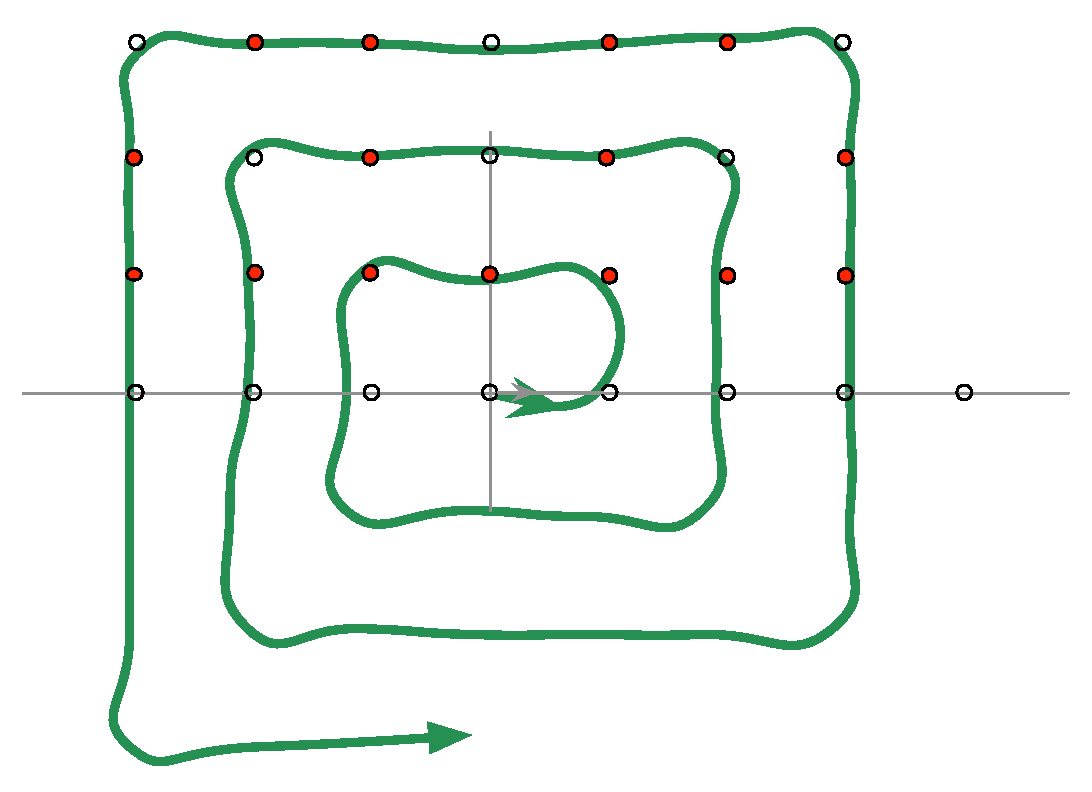
\includegraphics[width=6cm]{QN.eps} 
   \caption{I numeri razionali come punti del piano e ordinamento}
\end{figure}

Poi fate una spirale come quella in figura e ordinate i pallini che incontrate nell'ordine in cui li incontrate.
In pratica state costruendo una mappa $i:\N\arr \Q$. Siccome prima o poi passate per tutti i numeri razionali la mappa e biettiva e quindi $\N$ e $\Q$ hanno la stessa cardinalità.
La cardinalità di $\Q$ è infatti $\aleph_0$, i numeri razionali sono numerabili.

Notate che l'ordinamento che state definendo non è l'usuale ordinamento $q\le q'$ che non è un buon ordinamento, mentre quello che definisce la lista è (come quello di $\N$) un buon ordinamento. 

L'ordinamento di un insieme non è parte dell'insieme, uno {\it definisce} un ordinamento su un insieme e le definizioni sono libere, in un paese civile uno definisce le cose che vuole, basta che la definizione sia ben data.
Quindi $\Q$ può vestire ordinamenti diversi in situazioni diverse come voi potete cambiarvi la gonna senza smettere di essere voi.

Immaginate l'hotel di Hilbert con le stanze chiamate con nomi in $\Q$ e ordinate secondo l'ordinamento usuale lungo un corridoio.
Tra qualunque 2 stanze $q_1$ e $q_2$ ci sarebbero infinite camere $q$ con $q_1\le q\le q_2$ che darebbe all'hotel un aspetto molto più inquietante, vero?

\Note{Ok, tutto qui, basta che non mi chiediate a quale ordinale corrisponde il buon ordinamento che avete definito su $\Q$.
Se ci pensate la risposta è facile, avete tutto quello che serve per rispondere.
[per essere chiaro quando ho cominciato a scrivere questa frase non sapevo la risposta, volevo evitarla anche se stava davanti a me in piena luce.]
}


\section*{Giorno 17: numeri irrazionali (e trascendenti)}

Per il teorema di Pitagora, la lunghezza $d$ della diagonale di un quadrato è legata alla lunghezza $l$ del lato dalla relazione $d^2= 2 l^2$.
Ma che numero è $x=\frac[d/l]$ che deve soddisfare $x^2=2$?

\Note{Qui vi ho introdotto $x$ come una quantità geometrica apposta per non farvi dire semplicemente {\it non esiste soluzione}.
La diagonale avrà una certa lunghezza, giusto?
}

Ora mostriamo che non esiste nessun numero razionale $x=\frac[n/d]$ che soddisfa $x^2=2$. Abbiamo bisogno di un paio di ingredienti: intanto 2 è primo.

Secondo, se $2|n^2$ allora $4|n^2$.

\Note{
Se $2|n^2= nn$ allora, siccome $2$ è primo, $2|n$, cioè esiste un intero $k$ tale che $n=2k$, quindi $n^2=4k^2$, quindi $4|n^2$.
}

Terzo, possiamo supporre che $n$ e $d$ non hanno fattori comuni, se $k|n$ allora non $k|d$.

\Note{Se $k|n$ e $k|d$ possiamo semplificare la frazione e alla fine eliminare ogni fattore comune. Siccome basta eliminare i fattori primi comuni per eliminare qualunque fattore comune  si dice che 
possiamo assumere che $n$ e $d$ sono {\it coprimi}.}

Se $x^2=\frac[n^2/d^2]=2$ allora deve essere $n^2= 2d^2$ tra interi.

Quindi la nostra dimostrazione comincia con: supponiamo per assurdo che esista un numero razionale $x=\frac[n/d]$ con $n, d$ due interi coprimi tale che $x^2=2$, cioè
$n^2= 2d^2$.

Siccome $n^2=2d^2$, allora $2|n^2$, quindi $4|n^2$. Quindi esiste un intero $m$ tale che $n= 2m$ e quindi $4m^2=2d^2$ che semplificando un 2 diventa $2m^2=d^2$.
Quindi $2|d^2$, quindi $4|d^2$, quindi $2|d$ quindi esiste un intero $c$ tale che $d=2c$.
Quindi $d=2c$ è pari ($2|d$) e pure $n=2m$ ($2|n$) è pari.
Quindi, contrariamente a quanto ipotizzato, $n$ e $d$ hanno un fattore comune $2$, non possono essere coprimi.

L'unica via d'uscita (ma dovete essere convinti che l'ipotesi per assurdo è {\it l'unica} assunzione che abbiamo fatto) è che non è vero che $x$ è razionale.


\ms
Ora la storiella finisce che siccome la diagonale ha una lunghezza, ma questa non può essere razionale, devono esistere numeri (e.g.~$\sqrt{2}$) che non sono razionali.
Per ora non siamo in grado di definirli (sono i numeri reali, dentro i numeri reali ci sono anche i numeri razionali, mentre i numeri reali che non sono razionali si chiamano {\it irrazionali}).

\Note{I numeri irrazionali sono numeri che non si possono scrivere esattamente come con espressioni decimale. Vero. Ma pure $\frac[1/3]$ non può essere scritto esattamente in forma decimale, eppure e razionale. I numeri irrazionali sono numeri che non possono essere scritti come frazioni,  $\frac[1/3]$ può, $\sqrt{2}$ no.} 

Il numero irrazionale $\sqrt{2}$ è quindi la soluzione irrazionale dell'equazione $x^2=2$ che è un'equazione a coefficienti razionali (questa addirittura a coefficienti interi!).
Questo è particolarmente fastidioso. Abbiamo definito i numeri razionali $\Q$ e con questi possiamo scrivere equazioni $x^2=2$ che non hanno soluzioni in $\Q$.
Se la pensate così alzate le spalle e andate a fare merenda. Che problema può essere avere una equazione che non ha soluzione? Anche $x^2+1=0$ non ha soluzioni (neanche reali)
e questo è perfettamente naturale visto che $1+x^2 \ge 1$ di certo non può essere $1+x^2=0$!  
Pure l'equazione $3+ 0x=2$ non ha soluzione, ci certo $3= 3+0x$ non è uguale a $2$!

\Note{Un altro esempio di equazione senza soluzioni: $0x=1$. Che è il motivo per cui non abbiamo ammesso la frazione $\frac[1/0]$ tra i razionali.}

Non ci sarebbe nulla di strano ad avere equazioni che non hanno soluzioni. 
Se non fosse che come ho detto all'inizio che $d=\sqrt{2}$ è la lunghezza della diagonale di un quadrato di lato $l=1$.
Siccome faccio fatica a dire che questa quantità non esiste ho {\it scoperto} i numeri irrazionali, non li {\it invento}!

\Note{Ok, vi sto ammaliando di parole, il mio discorso è pubblicità, visto che posso anche dire che le equazioni senza soluzione esistono, quindi {\it invento} i numeri razionali, per dare un senso all'equazione che altrimenti non avrebbe soluzione. Ma il punto è proprio questo: entrambi i punti di vista sono difendibili e criticabili. Quindi non sono problemi veri sono solo opinioni linguistiche e retoriche!

Tra l'altro gli esempi di altre equazioni senza soluzioni li ho scelti apposta. L'equazione $x^2+1=0$ decidiamo di risolverla comunque e definisce i numeri complessi, mentre l'equazione $0x=1$
decidiamo di non risolverla e lasciamo $\frac[1/0]$ fuori dai razionali e da ogni altro insieme numerico che definiamo. Perché questo razzismo?

Perché se ammetto i numeri complessi posso estendere le operazioni e ottengo un {\it campo} più vasto dei numeri reali, mentre se ammetto $\frac[1/0]$ tra i numeri non riesco ad estendere in maniera ragionevole le operazioni aritmetiche. Non sono io che decido cosa scoprire, non so come gli alieni chiamano i campi, possono non averli ancora scoperti (e allora dubito siano in grado di costruire navi interstellari) oppure avere qualcosa di più generale (come noi abbiamo i campi che di sicuro sono inconcepibili ai romani). Ma se parlano di campi pure loro scoprono i numeri complessi e e reali, e i quaternioni (che sono solo un corpo visto che il prodotto non è commutativo).

Tra parentesi è falso che i campi sono inconcepibili per i romani! Ulrich {\it è un romano} e ha scoperto i campi come noi potremo scoprire quello che gli alieni avanzati usano al posto.}


Comunque approfittiamone per dare 2 nomi (che finora non ne abbiamo dati abbastanza). Pure $\pi$ è irrazionale (non che sia facile da dimostrare).
Peggio ancora non è soluzione di nessuna equazione che potete scrivere usando solo coefficienti in $\Q$ (che è ancora peggio da dimostrare). 
Quindi tra gli irrazionali, i numeri che non sono soluzioni di equazioni in $\Q$ come $\pi$, sono detti {\it trascendenti}.

Abbiamo già discusso (argomento diagonale di Cantor) che i numeri reali non sono numerabili (sono $\aleph_1$ per l'ipotesi del continuo).

Ora pensateci, gli irrazionali sono tanti quanti le equazioni che potete scrivere in $\Q$ che hanno un numero finito di coefficienti in $\Q$, cioè lasciatemelo dire male sono numerabili come $\Q$
(che andrebbe dimostrato che qui si cammina sulle sabbie mobili).
Quelli che rompono sono i trascendenti. Quasi tutti i numeri reali sono trascendenti nel senso che la cardinalità dei numeri irrazionali non trascendenti dovrebbe essere $\aleph_0$
sono i trascendenti i colpevoli per $\aleph_1$.

\Note{
come vi sembra ora il tesseract di Interstellar/Marvel?
}


\section*{Giorno 18: logica del prim'ordine}

Anche se non lo sappiamo, abbiamo un esempio di sistema assiomatico (gli assiomi di Peano per i numeri naturali) di un modello (i numeri naturali come cardinalità degli insiemi finiti).
Forse vale la pena di discutere un po' la semantica di tutto ciò.

\Note{Alcune cose che dirò sulla semantica della matematica sono opinioni personali. Quando quello che dico non è necessariamente condiviso provo a segnalarlo.}

Prima di dire cosa è un sistema assiomatico, serve un ambiente in cui sistemarlo. 
E questo ambiente, che chiamiamo {\it sistema formale}, è piuttosto familiare a chi fa informatica.
Poi specializziamo i sistemi formali in particolare al calcolo proposizionale (o logica proposizionale) e alla logica del prim'ordine.

\Note{Entrambi questi sistemi formali sono stati sviluppati per automatizzare il ragionamento nella seconda metà dell'1800.
Ci sono tante varianti ma alla fine in genera si usa quello che presentiamo come logica del prim'ordine.
}

Un {\it sistema formale} è fatto di:

un insieme finito chiamato {\it alfabeto} $\calA$ di caratteri, 

di liste di caratteri dette {\it parole}, che formano un vocabolario $\calV$, 

di frasi formate di parole secondo una ({\it context free}) grammatica.

\ms

Le frasi conformi alla grammatica si chiamano {\it predicati} o {\it proposizioni} a seconda del sistema formale che utilizziamo (vedi sotto).

Infine, abbiamo una lista di {\it regole di produzione}. 
Ogni regola di produzione è formata da $(n+1)$-predicati $(f_0, f_1, f_2, \dots, f_n)$.
I predicati $(f_1, f_2, \dots, f_n)$ si chiamano {\it premesse} o {\it ipotesi} della regola, mentre $f_0$ è detta {\it conseguenza} oppure {\it tesi}.
Una regola di produzione si indica come $[ f_1, f_2, \dots, f_n\arr f_0]$.

Le regole di produzione sono scelte in modo da automatizzare il ragionamento seguendo i principi della logica classica 
(o talvolta pure variazioni ad esempio la logica a più valori o altre varianti).

\Note{Un insieme di proposizioni è detto {\it chiuso} se quando contiene tutte le premesse di una regola di produzione, contengono pure la sua tesi.
Quindi se uno fornisce un insieme $\calP$ di proposizioni (assiomi), si può cercare di chiudere l'insieme $[\calP]$ 
applicando le regole di produzioni e aggiungendo le corrispondenti tesi.}

A noi interessano principalmente 2 esempi, che spiegano in modo semplice la definizione di sistema formale. 
Prima consideriamo la {\it logica proposizionale} e poi la {\it logica del prim'ordine} che in un certo senso è lo standard usato di solito.

Cominciamo con la logica proposizionale. 
Si intende che le proposizioni siano frasi (ad esempio nel linguaggio naturale) a cui si può attribuire un valore di verità, cioè sono o vere o false.
Non tutte le frasi sono così, {\it vai a cagare} o {\it vuoi più bene a mamma o a papà?} non sono proposizioni, 
{\it 10=3} o {\it Socrate è un uomo} sono proposizioni. Le proposizioni semplici (atomiche, che non contengono sotto-proposizioni sensate) si indicano con lettere latine maiuscole $A, B, \dots, P, Q, \dots$. Le proposizioni si possono poi combinare con i connettori logici, se $A$ e $B$ sono proposizioni, lo sono pure
$$
(A).and.(B)
\qquad
.not.(A)
\qquad
(A).or.(B)
\qquad
\dots
$$
Come sanno gli informatici tutti i connettori logici si possono definire utilizzando solo $(A).nand.(B) :=.not.( (A).and.(B))$.
Ad esempio, possiamo definire $.not.$ e $.or.$ come
$$
.not.(A)=(A).nand.(A)
\qquad
(A).or.(B)=   ( .not.( A )) .nand. ( .not. (B) )
$$
\Note{Potete controllare che questa definizione definisce $.or.$ davvero.
\begin{center}
\begin{tabular}{ccc}
$A$  & $B$ &  $(A).or.(B)$ \\
v & v &   v \\
v & f & v \\
f & v &  v \\
f & f &  f 
\end{tabular}
\end{center}

Forse bisogna specificare che esiste pure un operatore $(A)\then(B)$ che è definito come $(.not.(A)).or.(B)$.
Va detto perché siamo abituati a vederlo come una cosa logica che invece è definito come un operatore logico
\begin{center}
\begin{tabular}{ccc}
$A$  & $B$ &  $(A)\then(B)$ \\
v & v &   v \\
v & f & v \\
f & v &  f \\
f & f &  v
\end{tabular}
\end{center}

In pratica $(A)\then(B)$ è falso solo se $B$ è vero senza che lo sia $A$ che se ci pensate è l'unico caso in cui possiamo 
escludere che $B$ sia implicato da $A$ (se $A$ è vero deve essere vero pure $B$, se $A$ è falso allora $B$ è libero di fare quello che vuole).

}
 
Il riassunto è che potete creare tutti gli operatori logici che volete a partire dal $.nand.$ solamente.
Quindi se la grammatica specifica che 
$$
[Proposition] \arr [Proposition] .nand. [Proposition] 
$$ 
allora possiamo combinare proposizioni con ogni operatore logico.

Per noi $.not.(A)$, $(A).and.(B)$, $(A).or.(B)$, $(A)\then(B)$, \dots sono proposizioni se $A$ e $B$ lo sono.  


Le regole di produzione sono 
$$
[ (P)\then(Q), P  \arr Q]
\hbox to 6cm{\hfill (modus ponens)}
$$
da leggere: se $(P)\then(Q)$ e $P$ sono in $[\calP]$ allora è $Q$ in $[\calP]$.

Esempi delle altre regole sono
$$
\Align{
[ (P)\then(Q), .not.(Q)  \arr .not.(P)]&   \hbox to 5cm{\hfill (modus tollens)}\cr
[ (P).or.(Q), .not.(P)  \arr Q]&   \hbox to 5cm{\hfill}\cr
[P, Q \arr (P).and.(Q)] &\cr
\dots&
}
$$

Le regole di produzione sono abbastanza numerose (in fondo definiscono implicitamente tutti i connettori logici che sono $2^4=16$ tanti quante le tabelle di verità).
Ma il punto è la proprietà che si usa per sceglierle. Controllate pure, ma tutte sono valide indipendentemente dai valori di verità delle proposizioni che contengono.
In fondo se per giudicare se un ragionamento è corretto dovessimo sapere si cosa sta parlando non servirebbe la logica basterebbe applicare gli operatori logici.

\Note{Prendiamo come esempio il modus tollens $[ (P)\then(Q), .not.(Q)  \arr .not.(P)]$. Compaiono 2 proposizioni $P$ e $Q$ che possono essere entrambe, indipendentemente, vere o false.
\begin{center}
\begin{tabular}{cc}
$P$  	& $Q$		\\
v 	& v 		\\
v 	& f 		\\
f 	& v 		\\
f 	& f 		
\end{tabular}
\qquad\qquad
\begin{tabular}{ccc}
 $(P)\then(Q)$	& 	$.not.(Q)$	& $.not.(P)$	\\
  v 			&		f	&	f\\
  f 			&		v	&	f\\
  v 			&		f	&	v\\
  v 			&		v	&	v
\end{tabular}
\end{center}
Vedete che se le 2 premesse sono vere allora è vera pure la tesi.

Proviamo pure con $[P, Q \arr (P).and.(Q)]$
\begin{center}
\begin{tabular}{cc}
$P$  	& $Q$		\\
v 	& v 			\\
v 	& f 			\\
f 	& v 			\\
f 	& f 					
\end{tabular}
\qquad\qquad
\begin{tabular}{ccc}
$P$  	& $Q$	& $(P).and.(Q)$	\\
v 	& v 		&  v 				\\
v 	& f 		&  f 				\\
f 	& v 		&  f 				\\
f 	& f 		&  f 				
\end{tabular}
\end{center}
Di nuovo se le premesse sono vere allora la tesi è vera.

Come ho detto, non ho bisogno di sapere se le proposizioni sono vere o false. Diciamo che una regola è {\it valida} se e solo se la conseguenza è vera quando sono vere tutte le premesse
(non necessariamente quando sono vere $P$ e $Q$ che sono contenute nelle premesse).
}

Essere un ragionamento valido quindi non dice nulla del valore delle proposizioni che vi compaiono. 
In particolare, se abbiamo una premessa certamente falsa ($(A).and.(.non.(A))$) possiamo ricavare da questa in modo valido qualunque proposizione.


Se consideriamo un insieme chiuso $[\calP]$, se abbiamo che $A$ e $.not.(A)$ sono in $[\calP]$ allora l'insieme (o gli assiomi $\calP$ da cui deriva) è detto incoerente.
Un sistema di assiomi  è quindi  {\it coerente} se non consente di ricavare due proposizioni contraddittorie.


Se di ogni proposizione $A$ possiamo ricavare $A$ o $.not.(A)$ allora il sistema si dice {\it completo}.

Se nessun assioma può essere derivato dagli altri, il sistema si dice {\it indipendente}.

\ms

La {\it logica del prim'ordine} è un'estensione della logica proposizionale. Ha 2 ingredienti in più:

le variabili (indicate con lettere minuscole $x, y, \dots$) da cui i predicati $P(x)$ possono dipendere,

i quantificatori (per ogni $x$ ed esiste un $x$) che si può anteporre a un predicato per ottenere proposizioni.


\Note{
($P$: {\it 7 è primo}) è una proposizione, ($P(x)$: {\it x è primo}) è un predicato. Non possiamo dire se $P(x)$ è vera o falsa finché non sappiamo chi è $x$.
$P=P(7)$ è una proposizione, ma anche $\exists x: P(x)$ è una proposizione che afferma che esiste (almeno) un numero primo, mentre $\forall x:P(x)$
è una proposizione (falsa) che afferma che tutti i numeri naturali sono primi.
In genere le variabili $x, y$ sono elementi di un insieme (e.g.~$x\in \N$) che è l'ambito in cui stiamo lavorando.
}

Sia la logica proposizionale che la logica del prim'ordine hanno 2 scopi, quello di rappresentare i ragionamenti (come lo spartito rappresenta la musica)
e quello di definire i ragionamenti validi, cioè quelli che garantiscono che {\it se sono vere le ipotesi allora è vera pure la tesi}.

Il prossimo passo è specificare quest'ambito (la logica del prim'ordine) i sistemi assiomatici e i modelli.


\section*{Giorno 19: sistemi assiomatici}

Un sistema assiomatico è costituito da:

{\it termini indefiniti}: un insieme di parole assunte senza definizione.

{\it assiomi}: un insieme di enunciati assunti senza dimostrazione.

{\it un sistema formale}: per derivare nuovi enunciati da quelli noti, in genere assumiamo la logica del prim'ordine.

{\it definizioni}: si possono definire nuovi termini fornendone una definizione univoca in termini di assiomi, termini primitivi e teoremi disponibili ad un dato momento per evitare circoli viziosi.

{\it teoremi}:  sono enunciati che possono essere scritti in termini di termini primitivi, assiomi, definizioni e teoremi disponibili ad un cero momento.
 Un teorema deve essere derivato da assiomi e teoremi per mezzo delle regole di produzione della logica del prim'ordine.
 Una tale derivazione si chiama dimostrazione.
 
 \Note{ Un teorema non è un enunciato, è un enunciato {\it con una dimostrazione}.
 La logica del prim'ordine è usata esattamente come canone per derivare nuovi enunciati da quelli noti (assiomi o teoremi).
 La derivazione è esattamente una lista di enunciati prodotti usando le regole di produzione specificati nella logica del prim'ordine.
 
 Lasciatemi sottolineare che le regole di produzione che abbiamo specificato sono fatte per collegare enunciati tra loro in nodo che siano {\it validi},
 cioè che non si può verificare mai che la conseguenza sia falsa se tutte le premesse sono vere. La validità non chiede che le premesse siano vere, non afferma che la tesi è vera.
 Le regole di produzione sono espresse nella logica del prim'ordine in cui gli enunciati sono rappresentati da costanti proposizionali, 
 cioè lettere (tipo $P$) che rappresentano  proposizioni specifiche. Nella logica del prim'ordine equando si discute la validità non avete neanche a disposizione cosa dicano gli enunciati che si stanno collegati.
 
 Questo è un fatto. Quando scriviamo che $1+1=2$ lo dimostriamo definendo $1=s(0)$ e $2=s(1)$ e poi si usa la definizione di somma $a+s(b)= s(a+b)$ (definizione somma) e $a+0=a$ (definizione 0) oltre agli assiomi di Peano.
 \eq{
 \Align{
  \hbox to 3cm{$1+1= 1+s(0)$\hfill }  \qquad\qquad\qquad \hbox to 3cm{(definizone 1)\hfill}\cr
  \hbox to 3cm{$1+1= s(1+0)$\hfill }  \qquad\qquad\qquad \hbox to 3cm{(definizone somma)\hfill}\cr
  \hbox to 3cm{$1+1= s(1)$ \hfill}  \qquad\qquad\qquad \hbox to 3cm{(definizone 0)\hfill}\cr
  \hbox to 3cm{$1+1= 2$\hfill }  \qquad\qquad\qquad \hbox to 3cm{(definizone 2)\hfill}\cr
 }
 }
 non abbiamo nessun vantaggio sostanziale a sapere cosa sono 1, 2, +, 0, $s$. Tra l'altro $s$ è una relazione indefinita, 0 è detto esistere da un assioma, 1, 2
 sono termini definiti.
 }

 


Un sistema assiomatico può presentare delle patologie.

Se in un sistema non posso dimostrare risultati contraddittori (ad esempio 
\eq{
(P).and.(.not.P)
}
che è sicuramente falso) il sistema (gli assiomi) è {\it coerente}.

Se in un sistema di qualsiasi enunciato posso dimostrare $P$ oppure $.not.(P)$ il sistema (gli assiomi) si dicono {\it completi}.

Se in un sistema non posso dimostrare un assioma, allora il sistema (gli assiomi) si dice {\it indipendente}.


La completezza e l'indipendenza sono auspicabili, ma la coerenze è necessaria.
In un sistema incoerente, abbiamo dimostrato un enunciato sicuramente falso, e si può mostrare che uno può derivare qualunque enunciato da una ipotesi sicuramente falsa.
Abbiamo riconosciuto che la validità di una dimostrazione è riposta nell'assicurare che la tesi non può essere falsa se le ipotesi sono vera. Ma se le ipotesi sono sicuramente false, non c'è nulla da assicurare. Da una premessa falsa segue qualunque cosa.

Quindi in un sistema assiomatico incoerente ogni proposizione è dimostrabile e un tale sistema quindi non serve a nulla.
Forse possiamo dire che lo scopo della matematica non è di dimostrare che le cose sono vere e nel produrre dimostrazione di tali enunciati (fosse questo basterebbe un unico sistema formale incoerente) ma si sapere che alcuni sono falsi.
Per questa ragione la coerenza è necessaria, della completezza e dell'indipendenza possiamo fare a meno.

Quando guardiamo ad un teorema, l'unica cosa che sappiamo che non può capitare è che la tesi sia falsa quando tutte le ipotesi sono vere.
Se le ipotesi sono state dimostrate anch'esse, la tesi è vera {\it se sono veri gli assiomi}. 

La matematica non parla di vero o falso parla di dimostrabilità di enunciati, che loro possono essere veri o falsi.
Sapere che un enunciato può essere dimostrato non ci dice se questo è vero o falso, ci dice che deriva dagli assiomi. Se chiedete a me non sapete neanche che gli assiomi sono veri o falsi, sapete che li assumete validi senza dimostrazione. Assumere una cosa per valida, non significa che la ritenete vera, significa che la ritenete valida senza dimostrazione.

In questo contesto, ditemi voi cosa serve il significato dei termini indefiniti?
Voi conoscete Socrate? Avete mai visto un triangolo al supermercato? Un numero?

La matematica non sono non parla del mondo reale, non parla neanche di vero e falso, parla solo si enunciati validi cioè di quali enunciati possono essere dimostrati a partire dagli assiomi.
È il prezzo che si paga se si vuole avere certezze, possiamo avere certezze sul nulla oppure non sapere nulla di tutto.

\Note{
Quando sono state scoperte o inventate le geometrie non euclidee sono state prodotte modificando il quinto postulato di Eulcide (per un punto fuori da una retta passa un'unica parallela)
in altri assiomi in contraddizione con esso (ad esempio: non esistono parallele oppure per un punto esistono infinite parallele).
Poi si vede che le geometrie non-euclidee sono coerenti tanto quanto quelle Euclidee.

Ora se gli assiomi dovessero essere veri come fanno ad essere veri assiomi contraddittori anche se in sistemi assiomatici diversi?

Se ne esce solo dicendo che in certi casi valgono gli assiomi di Euclide talvolta gli altri. 
Si sopravvive solo dicendo che la validità non parla di verità e falsità, un enunciato non è valido o non valido, è valido in un sistema formale e magari non valido in un altro.
}

Se fate un giro su Wiki vedete che si usa un sacco di vero e falso. 
La mia {\bf opinione} è che questa semantica sia comoda per noi ma non sta scritta nella matematica. La matematica è senza significato, non parla di vero o falso parla di quali proposizioni possono essere derivate da altre.
La matematica è una questione di relazioni tra enunciati che chiamiamo validità e che descriviamo dando una dimostrazione.



\section*{Giorno 20: modelli}

Finora abbiamo visto un sistema assiomatico (gli assiomi di Peano per gli ordinali naturali).
Questo è fatto come descritto ieri. 
Il {\it successivo} e {\it numero naturale} sono termini indefiniti.
Gli assiomi sono quelli che abbiamo scritto.
Abbiamo definito somma e prodotto e abbiamo dimostrato alcuni teoremi ($5+3=8$).

Lo abbiamo fatto in modo un po' informale, secondo i canoni della logica del prim'ordine e i sistemi di dimostrazione annessi
avremmo dovuto annotare una lista di enunciati e con quale regola di produzione è stata prodotta a partire da quali premesse.
Ma noi siamo fighi e ribelli e facciamo le cose come ci pare.

Da quello che abbiamo detto in realtà manco sappiamo cosa significa successivo e numero naturale. 
La semantica è suggerita dai nomi, aiuta ma non è necessaria e non segue dagli assiomi né dai teoremi successivi.

Possiamo dire che gli assiomi si {\it inventano} ma una volta fissati gli assiomi in linea di principio i teoremi che da questi si possono dimostrare sono stabiliti per sempre anche se noi ancora non li conosciamo. 
Una volta stabiliti gli assiomi, noi certamente {\it scopriamo} le dimostrazioni e i teoremi.

Abbiamo anche discusso che i sistemi assiomatici possono essere coerenti, indipendenti e completi.
G\"odel ha dimostrato che il sistema di Peano non è completo. Ci sono enunciati che non possono essere dimostrati vero o falsi (tra cui la coerenza).

Ma chi ci garantisce che è un sistema coerente? Chi ci assicura che domani non scopriremo che $1=0$? (Già un assioma ci dice che $1:= s(0)\not=0$.)

Per alcuni sistemi assiomatici molto semplici qualche volta questo è possibile dimostrarlo direttamente nel sistema stesso. 
Ma G\"odel ci assicura che la coerenza in Peano non è decidibile.

Altre volte (e pure per Peano) è possibile dare una prova relativa di coerenza fornendone un modello.

Un modello consiste nel considerare un altro sistema assiomatico (in genere più complesso di quello che stiamo analizzando).
Nel sistema grande (nel caso di Peano il sistema assiomatico di teoria degli insiemi) noi possiamo trovare oggetti (insiemi) che realizzano i termini indefiniti di Peano
in modo che gli assiomi diventano teoremi nel sistema grande.

\Note{
Potete definire $0$ come l'insieme $\Emptyset$. E noto $n\in \N$ come insieme possiamo definire il successivo come l'insieme $s(n)= n\union \{n\}$.
Poi possiamo dimostrare come teoremi in teoria degli insiemi che valgono gli altri assiomi come teoremi.

Fatto questo abbiamo un modello del sistema assiomatico di Peano all'interno di teoria degli insiemi.
Se, {\bf se}, teoria degli insiemi è coerente allora Peano è coerente, per questo si chiama dimostrazione relativa di coerenza.
} 


In un modello c'è una semantica interna alla teoria grande del sistema piccolo. È tutto meno astratto, ma in genere la teoria grande è altrettanto possibile sia incoerente rispetto alla teoria piccola. 
Nella teoria degli insiemi uno {\it scopre} gli assiomi di Peano come teoremi.

Talvolta il medesimo sistema può avere modelli diversi anche in teorie diverse.

Notate che invece per definire interi e razionali, abbiamo preso un'altra strada.
Non abbiamo definito un nuovo sistema assiomatico, Abbiamo esteso con definizioni il sistema di Peano.
Noi lo abbiamo fatto usando il suo modello ma possiamo dimostrare tutto come teoremi in Peano.
Se facciamo finta di sapere cosa è un numero naturale, abbiamo un modo di scoprire i numeri interi e razionali. 
Noi diamo delle definizioni ma la possibilità di considerare coppie di naturali (o interi) e la possibilità di scegliere operazioni su questi nuovi  numeri è già implicita negli assiomi di Peano. 


Questi si chiamano modelli, poi possiamo specificare una specie di modelli materiali in cui i termini indefiniti vengono associati a oggetti reali e gli assiomi a loro proprietà.
In questo senso talvolta si interpretano gli oggetti matematici come oggetti reali e gli assiomi come le loro proprietà.
Questi sistemi materiali sono il fondamento dell[uso della matematica nelle scienze naturali. {\bf Secondo me}, non sono matematica nel senso di cui sopra.
Per sapere se un oggetto reale ha una proprietà occorre fare un esperimento, non una dimostrazione.

Il meccanismo alla base dei sistemi materiali è interessante, ne parliamo un'altra volta, ma secondo me un po' oltre la matematica e spostato nella direzione delle scienze naturali.


\newpage
\NewSection{Quinta settimana}

Vediamo l'avvento dell'algebra, impariamo a risolvere equazioni di primo e secondo grado.


\section*{Giorno 21: Algebra e equazioni}

Nel 1200 arrivano in europa i numeri che gli arabi avevano imparato dagli indiani.
In quel periodo gli arabi si trovavano ad avere lo stesso ruolo di porta dell'europa verso oriente che avevano avuto i greci durante l'antichità.

Come i greci avevano importato in europa la geometria imparata da balilonesi e egiziani arricchendola del concetto di dimostrazione
così gli arabi-persiani importarono lo zero, la notazione posizionale, arricchendo il tutto con l'agebra.

Nel 300ac Euclide colleziona molti risultati noti e li deriva da un insieme di postulati assunti per veri.
Per 2300 anni gli elementi di Euclide, il suo stile di dimostrazione, sono stati il prototipo e la definizione di cosa significava matematica in europa.
Gli elementi di Euclide sono stati copiati, integrati e estesi per tutto questo periodo senza che nessuno (prima di Hilbert) si osasse a metterne in discussione 
la struttura.

\Note{all'inizio del 1800 Gauss --inedito--e poi altri hanno proposto le geometrie non euclidee, essenzialmente per mostrare che il quinto postulato di Euclide era indipendente dagli altri.
Alla fine dell'800 Hilbert invece proponeva una versione migliorata degli elementi di Euclide aggiungendo un po' di assiomi che da Euclide erano stati assunti e usati senza annotarli esplicitamente. Tale aggiunta era necessaria per poter portare gli elementi allo standard che stava  emergendo dalla logica matematica in quel periodo: nessuna assunzione implicita, nessuna ambiguità semantica.

Ci sono voluti 2300 anni per poter dire che gli elementi non erano del tutto perfetti, e ci è voluto Hilbert (e Gauss prima di lui).}
  
Nei nuovi numeri c'era lo zero e i numeri interi, anche se i numeri negativi impiegarono qualche secolo a diventare di uso comune tranne in finanza dove erano usati per rappresentare i debiti o le perdite. Gli arabi li usavano in finanza ma non in algebra, in India erano usati con circospezione ma pare fossero stati inventati in Cina.
A partire dal 1200 in europa, a opera principalmente di Fibonacci si cominciò a diffondere la nuova notazione (con lo zero e posizionale).

Ma quello che gli arabi aggiunsero è stata l'algebra (ad opera di Al-Khwārizmī che era persiano), cioè la capacità di risolvere problemi, quelli che noi oggi riconosciamo come equazioni di primo e secondo grado.
All'inizio per gli arabi l'algebra era una disciplina parlata. Risolvevano un problema con un discorso tipo

\Note{Cos`è il quadrato di una cosa che, quando incrementato di 10 volte la sua radice, è uguale a 39?
La soluzione è questa: dividi in due il numero di radici, che in questo caso dà 5.
Questo moltiplicato per se stesso è 25. Aggiungi questo a 39; la somma è 64. 
Ora prendi la radice di questo, che è 8, e sottrai da ciò metà del numero delle radici, che è 5; il resto è 3.
Questa è la radice del quadrato che stavi cercando.

Se tenete traccia e partite dall'equazione $x^2+bx=c$ ottenete la descrizione della formula
\eq{
x=\sqrt{\(\frac[b/2]\)^2+c}-\frac[b/2]
}
che è la formula (ridotta che usiamo per risolvere le equazioni di secondo grado ponendo $a=1$.)

[Notate niente numeri negativi, non scrive $x^3+10x-39=0$ proprio per non parlare di numeri negativi.]
}


Successivamente hanno inventato una notazione un po' complicata per trattare questi problemi. 
Scrivevano $.3.^2p.12 egaulx a .9.^1$ per quello che noi oggi scriviamo $ 3x^2 + 12 = 9x$ (sempre evitando i numeri negativi).

Noi sappiamo veramente poco di quello che si faceva a quei tempi.

\Note{Come dice John Dersch le cantine delle moschee del medio oriente devono essere piene di manoscritti di quel periodo che raccontano come è nata l'algebra, ma purtroppo a nessuno importa.}
 
Anche perché in europa (ma pure nel mondo arabo) tutto ciò aveva poco interesse teorico e maggiormente un interesse pratico per mantenere i conti dei mercanti in ordine. 
Prevaleva un atteggiamento pragmatico. Se le dimostrazioni di Euclide finivano con la formula medievale QDE ({\it quod erat demonstrandum} ciò che si doveva dimostrare)
le {\it dimostrazioni} algebriche finivano in una formula equivalente a {\it e vedrai che questo è il numero che cercavi}.
Se le dimostrazioni di Euclide bastavano a loro stesse, riponevano il loro valore nel metodo, quelle dell'algebra rimandavano a una verifica. Erano problemi in cui ti do un metodo per calcolare il risultato che non è necessario tu capisca o trovi convincente e poi, se ti va, una volta trovato il risultato puoi verificare che questo è la soluzione che cercavi.
Questo anche perché i problemi dell'algebra sono strutturalmente così: sono problemi in cui è difficile trovare il risultato ma è facile verificare se un numero è la soluzione cercata. 

\Note{Se vi è famigliare la sensazione di dover applicare una formula non avendo capito da dove salta fuori, bene è cominciato tutto là. Anche in europa l'algebra è rimasta per secoli divisa dalla vera matematica e solo verso il 700-800 è stata assiomatizzata al punto di poter dimostrare le formule alla stregua di quello che faceva Euclide.
La diffidenza secolare per i numeri negativi viene anche da fatto che molte formule erano dimostrate geometricamente, e in geometria ciaone numeri negativi. Ad esempio 
$a^2+b^2+2ab = (a+b)^2$ era {\it dimostrata} dalla figura

$$   
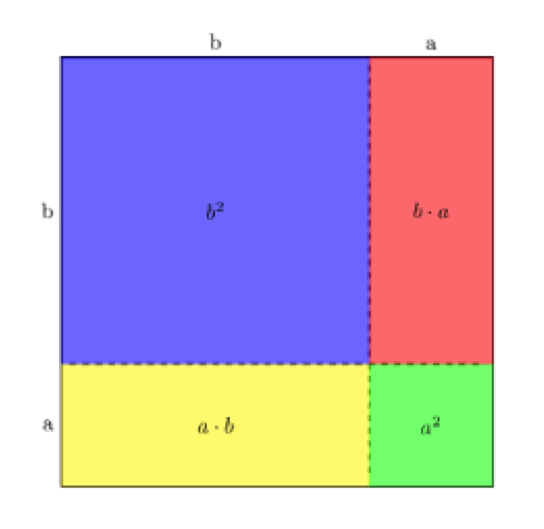
\includegraphics[width=6cm]{quadrato.eps} 
   %\label{fig:example}
$$
\centerline{ {Figura 1: $a^2+b^2+2ab = (a+b)^2$}}

}

Un altro aspetto delle verifiche è che non è richiesta una astrazione ulteriore rispetto a saper fare i conti per la verifica.
Io posso trovare una formula per un qualunque polinomio di secondo grado $ax^2+bx+c=0$, te la racconto su un esempio $2x^2+6x+10=0$,
e poi ti dico di verificare il risultato. Infine ti informo che puoi usare la stessa tecnica in generale per qualunque polinomio di secondo grado.
Tu applichi la stessa formula che avevi imparato per l'esempio anche senza capirla e poi verifichi che il risultato che trovi è giusto.
Se non ti viene la verifica, siccome la formula l'ho detta io e tu non sei un cazzo, significa che hai sbagliato tu, trovati l'errore.
Il tutto senza doverti dire cosa è l'algebra letterale con cui io faccio il conto.

\Note{Nel mondo anglosassone anche nelle discipline dure, il calcolo differenziale è ancora oggi insegnato così. Uno si fa il corso di calculus in cui impara a calcoare le derivate e gli integrali senza capire nulla. Poi si fa il corso di Analysis in cui si dimostrano i teoremi necessari a capire quello che si è imparato a fare. Per me pessima idea e un pessimo esempio di controeducazione civica. Ma è così. Questo è per me il secondo motivo per cui dovrebbe essere vietato insegnare matematica come è insegnata nella maggior parte dei casi.
}


Quindi dal 1200 ad almeno tutto il 1600 la matematica è la storia di una coppia di separati in casa, e di conseguenza la didattica della matematica un disastro.

Ora il nostro prossimo obiettivo è quello di arrivare a risolvere le equazioni di primo e secondo grado in generale.
La buona notizia è che se vi ricordate la definizione di relazione di equivalenza non avete bisogno di altro.


\section*{Giorno 22: lettere, incognite e parametri}

Una volta che abbiamo imparato a fare le operazioni con i numeri razionali, che contengono pure gli interi e i naturali come casi particolari,
in molte situazioni vogliamo scrivere identità che valgono per ogni valore dei numeri coinvolti.
Per questa ragione abbiamo inventato i parametri $a, b, c, \dots\in \Q$.
Quando ad esempio scriviamo le proprietà delle operazioni
\eq{
a(b+c)= ab+ac
}
intendiamo che questa vale per ogni valore di $a, b, c\in \Q$. 

Tra breve introdurremo le incognite che di solito indichiamo con $x$ che hanno una semantica diversa. Quando scriviamo 
\eq{
3x+3=1-2x
}
intendiamo chiedere se esiste un valore di $x$ che rende uguali i 2 lati dell'equazione.
I {\it parametri} sottintendono un quantificatore universale (per ogni) mentre le {\it incognite} sottintendono un quantificatore esistenziale.
Se vi aiuta, le incognite hanno un valore interrogativo aggiunto: esiste un valore di $x$ per cui è verificata l'equazione?

\Note{Quindi quando scriviamo 
\eq{
\frac[a+b/a]=b
}
non basta vedere che per $b=2$ e $a=2$ è soddisfatta per accettarla come formula valida, 
mentre basta vedere che non vale per $a=1$ e $b=2$ per dire che l'identità non è corretta.
}

Ora se state pensando che distinguere tra parametri e incognite è facile, se vedo $x, y, z, \dots$ sono incognite se vedo $a, b, c, \dots$ sono parametri anche questo non è sempre vero.
Se vi chiedo di scrivere l'equazione della retta generica mi scrivete $ax+by=c$ intendendo che per ogni valore di $[a,b,c]$ che sono parametri,
i punti $(x,y)$  che soddisfano l'equazione si distribuiscono lungo una retta, quale retta è identificata dai parametri, mentre $x, y$ compaiono come incognite.

Se poi chiediamo quali rette passano per il punto $(2, 3)$, dobbiamo sostituire a $(x, y)=(2, 3)$ ottenendo $2a+3b=c$ e a questo punto dobbiamo determinare $(a, b,c)$ in modo che questa identità sia valida. Le lettere $a,b,c$ che nel paragrafo precedente erano parametri, ora diventano incognite. Allora si determina $c=2a+3b$ e si sostituisca
\eq{
ax+by=2a+3b
\qquad
a(x-2)+b(y-3)=0
}
che di nuovo, per ogni valore $[a,b]$ determinano una retta che passa per il punto $(2,3)$.
Quindi $a, b$ tornano parametri e $x, y$ tornano incignite.

In pratica è il lettore in base a quello che vuole fare che decide cosa è parametro e cosa è incognita.


È ovvio che per fare i conti con frazioni qualunque non serve fare i conti coi numeri ma bisogna vedere il calcolo come manipolazione di formule seguendo delle regole 
che derivano dalle proprietà delle operazioni
\eq{
\frac[a/b]+ \frac[c/d]=\frac[ad+cb/bd]
\qquad\qquad
\frac[a/b] \frac[c/d]=\frac[ac/bd]
\qquad\qquad
\frac[{\frac[a/b] }/{  \frac[c/d]}]= \frac[a/b]\frac[d/c]
}

\Note{Queste sono le stesse regole che si usano nel caso delle frazioni numeriche, tranne il fatto che per evitare di dover semplificare alla fine (cosa che peraltro può succedere comunque)
quando sommiamo le frazioni si cerca nel caso numerico il minimo comune denominatore, mentre nel caso letterale, visto che non sappiamo i valori non possiamo di certo sapere il minimo comune denominatore e quindi lo facciamo prendendo come denominatore semplicemente il prodotto. 
}

Anche questo passaggio dai numeri alle lettere è un passaggio delicato e qualcuno non lo passa mai.
Intanto dovete scordarvi che sia
\eq{
\frac[a+b/a]=b
\qquad\o\qquad
\frac[a+b/a]= 1+b
}
Potete facilmente convincervi che queste formule non sono valide, fatelo.

La seconda cosa importante sono le regole di precedenza tra le operazioni. 
Tutto nasce dal fatto che per specificare l'ordine con cui vengono applicate le operazioni, bisognerebbe scrivere
\eq{
\frac[1+3+4/8] = (1+(3+4))/8
}
Prima si svolgono i conti nelle parentesi più interne quindi si calcola
\eq{
\frac[1+3+4/8] = (1+(3+4))/8
=  (1+7)/8
= 8/8
=1
}

Ciò comporta che, non fosse per la proprietà associativa della somma, non si potrebbe neanche scrivere $1+3+4$ perché sarebbe ambiguo distinguere tra $(1+3)+4$ e $1+(3+4)$.
È solo in virtù della proprietà associativa che  $(a+b)+c=a+(b+c)$ e quindi, non essendoci differenza tra le 2 scritture, possiamo scrivere ancora peggio $a+b+c$.
La stessa cosa per il prodotto $abc$.

Ma il problema emerge comunque quando si mischiano somme e prodotti. Se scriviamo $a+bc$ intendiamo
$a+(bc)$ o $(a+b)c$?

\Note{Notate che sui libri $a+bc=a+(bc)$ mentre sulle calcolatrici
$a+bc$ calcola $(a+b)*c$. 
Le calcolatrici calcolano le funzioni nel valore che compare sullo schermo, calcolano e operazioni tra il valore sullo schermo e il successivo valore digitato.

Almeno di norma perché poi esistono calcolatrici bellissime in polacco inverso in cui per calcolare 5+3 si digita 3 5 + (come in forth o nel linguaggio che si usa per i compilatori)
o in polacco diretto in cui si digita + 5 3 (come in lisp in ps o in pdf).
In più oggi la potenza di calcolo è sufficiente per implementare sulle calcolatrici le convenzioni dei libri con la possibilità di scrivere una formula su una riga con tutte le parentesi necessarie
e poi interpretarla e calcolare il risultato. Questo succede su molti smartphones ma ad esempio le calcolatrici di sistema di windows implementano le convenzioni standard delle calcolatrici standard.
}

Non so perché i lettori siano allergici alle parentesi, ma per evitarle si conviene che il prodotto abbia precedenza sulle somme, quindi
\eq{
a+bc=a+(bc)
}
mentre se uno vuole può scrivere $(a+b)c$ in cui la parentesi è necessaria se prima si vuole fare la somma e poi il prodotto.

La stessa  cosa le potenze hanno la precedenza sui prodotti. di norma si interpreta $xy^2= x\cdot (y^2)$ non come $(xy)^2$.

Onestamente sono cose che abbiamo assunto col latte materno e farei fatica a fare una lista delle precedenze adottate in matematica.
Le abbiamo assunto facendo una serie interminabili di esercizi tipo semplificare l'espressione
\eq{
\Frac[(x-y)(x+y)/xy]+ \Frac[2y/x]+2-\Frac[(x+y)^2/xy]
}
in cui tra l'altro $x, y$ compaiono come parametri.
Semplificare una espressione significa riscriverla in modo più semplice, riscrivendo sempre espressioni uguali.

\Note{
Semplificare l'espressione 
\eq{
\Align{
&\Frac[1/x^2-4x+4]- \Frac[2/x^2-2x] +\Frac[1/x^2-x-2]=\cr
&\quad=\Frac[1/(x-2)^2]- \Frac[2/x(x-2)] +\Frac[1/ (x-2)(x+1)]=\cr
&\quad=\Frac[x(x+1)/x(x+1)(x-2)^2]+\Frac[-2(x+1)(x-2)/x(x+1)(x-2)^2]+ \Frac[x(x-2)/x(x+1)(x-2)^2]=\cr
&\quad=\Frac[x(x+1)  -2(x+1)(x-2)	 +x(x-2)		/x(x+1)(x-2)^2]=\cr
&\quad=\Frac[x^2+x  -2x^2+2x+4+x^2-2x 		/x(x+1)(x-2)^2]=\cr
&\quad=\Frac[  x+4		/x(x+1)(x-2)^2]\cr
}
}
L'esercizio prende la forma di una catena di uguaglianze tra espressioni equivalenti piano piano più ``semplici''.
}

Assicuratevi di saperla semplificare, saperla calcolare ponendo $x=7$ e $y=-4$.
Questo è un buon posto per fermarsi se non siete super-convinti di saperlo fare. 
Se cercate {\it esercizi espressioni algebriche letterali} trovate un miliardo di esercizi da svolgere.

Esercitatevi, scoprite dove siete soliti fare errori, condizionatevi a controllare mentre fate i conti di non aver fatto errori. 
È una forma di meditazione e solo così potete ottenere di riuscire a eliminare gli errori che condizionano il risultato.
Se l'espressione si allunga e siete esposti a fare un errore ogni 100 passaggi, da una certa complessità in sù sarete pressoché certi di ottenere un risultato sbagliato, e non potete permettervelo.

Dice il saggio: 
\blockquote{\footnotesize
It was never really a battle for me to win, \\
it was an eternal dance\\
And like a dance, the more rigid I became, the harder it got\\
The more I cursed my clumsy footsteps, the more I struggled

So I got older and I learned to relax\\
And I learned to soften and that dance got easier

It is this eternal dance that separates human beings\\
From angels, from demons, from gods\\
And I must not forget, we must not forget\\
That we are human beings\\
}

Può essere fatto, potete diventare sicuri del conto che avete fatto, anche se è lungo una pagina.

\section*{Giorno 23: equazioni lineari}

Una equazione sono 2 espressioni (che possono contenere incognite) poste uguali tra loro.

\Note{È un'equazione $3x+2=2x$.
Ma pure $2x+3y-4=3x=2y+1$.

Siccome 0 è essa stessa una espressione, $3x-1=0$ è anche un'equazione.
Più semplicemente, prediamo una funzione $f:\Q^n\arr \Q: (x_1, x_2,\dots, x_n)\mapsto f(x_1, x_2,\dots, x_n)$ a cui è associata l'equazione $f(x_1, x_2,\dots, x_n)=0$.

In particolare $0=0$  (oppure $x=x$), è soddisfatta da ogni valore di $x$, quindi qualunque valore di $x$ è soluzione.

Invece non c'è nessun valore di $x$ per cui $1=0$ (oppure $x+1=x$), che quindi è un'equazione senza soluzione. (Questa non ha soluzione è uno degli assiomi di Peano, tra l'altro.
Ma allora l'abbiamo dimostrato? Certo, ma abbiamo assunto una paccata di assiomi tra cui quelli di Peano. Abbiamo detto che gli assiomi sono assunti per validi in un sistema formale e se abbiamo un modello diventano teoremi in un sistema assiomatico più grande.)

Se vi chiedo di risolvere $ax+b=0$ dovrei specificare quali sono le incognite e quali i parametri anche se in genere si intende che $x,y, z, \dots$ sono le incognite.
}
 
Due equazioni sono dette {\it equivalenti} se hanno le stesse soluzioni, cosicché risolvere l'una o l'altra non fa differenza.
Risolvere una equazione significa scrivere una lista di equazioni equivalenti che alla fine diventano $x=5$ (oppure $0=0$ o $1=0$) che rendano manifesti i valori dell'incognita che soddisfano l'equazione.

Quindi l'unica cosa veramente rilevante è capire quando 2 equazioni sono equivalenti.

\Note{
Sia data un'equazione $f(x)=g(x)$. Se sommiamo ad ambo i membri una stessa funzione $h(x)$ otteniamo una equazione $f(x)+ h(x)= g(x)+ h(x)$ che è equivalente all'equazione di partenza.

Infatti se $x=x_0$ è soluzione della prima $f(x_0)=g(x_0)$, allora abbiamo anche che $f(x_0)+ h(x_0)= g(x_0)+ h(x_0)$.
Viceversa, se  $f(x_0)+ h(x_0)= g(x_0)+ h(x_0)$ ovviamente $h(x_0)=h(x_0)$ e quindi deve essere $f(x_0)= g(x_0)$.
Quindi $x_0$ è soluzione della prima se e solo se è soluzione della seconda.

Consideriamo ora l'equazione $f(x)h(x)=g(x)h(x)$.
Se $x=x_0$ è soluzione della prima $f(x_0)=g(x_0)$, allora abbiamo anche che $f(x_0)h(x_0)= g(x_0)h(x_0)$ (purché $x_0$ sia nel dominio di $h(x)$).
Viceversa, se  $f(x_0)h(x_0)= g(x_0)h(x_0)$ ovviamente $h(x_0)=h(x_0)$ e quindi, se $h(x_0)\not=0$, deve essere $f(x_0)= g(x_0)$.
Ma se $h(x_0)=0$, allora $f(x_0)h(x_0)= g(x_0)h(x_0)$ anche se $f(x_0)\not= g(x_0)$.
Quindi $x_0$ è soluzione della prima se (ma non solo se) è soluzione della seconda.
Le 2 equazioni non sono equivalenti (a meno che la funzione $h(x)$ non sia priva di soluzioni).

Quando moltiplichiamo e dividiamo per qualcosa che dipende dalle incognite possiamo introdurre con ciò delle soluzioni della seconda equazione che non erano soluzioni della prima.
Si può fare ma se lo facciamo poi dobbiamo verificare che i valori trovati siano stati soluzioni della prima equazione per eliminare le soluzioni spurie.

Ma se moltiplichiamo o dividiamo una equazione per una costante non nulla allora sicuramente otteniamo un'equazione equivalente (proprio perché la costante non nulla è anche una funzione che non si annulla mai.)

Più in generale se applichiamo la stessa funzione ad ambo i membri $h(f(x))= h(g(x))$ otteniamo una equazione equivalente se $h$ è biettiva.
Se $h$ non è biettiva possiamo introdurre delle soluzioni spurie. Alla fine dobbiamo quindi verificare le soluzioni trovate per eliminare le eventuali soluzioni spie.
Ad esempio consideriamo $x-1=3-2x$ (che ha come unica soluzione $x=\frac[4/3]$) e invece di risolverla semplicemente applichiamo il quadrato ad ambo i membri
$x^2-2x+1= 4x^2-12x+9$ che si semplifica a $3x^2-10x+8=0$.
Questa si fattorizza come $\(x-\frac[4/3]\)\(3x-6\)=0$. (Ora non vi preoccupate di come io abbia fattorizzato, preoccupatevi che la fattorizzazione sia giusta, verificando che il prodotto dà quello che c'era.)

Quest'ultima equazione ha 2 soluzioni, $x=\frac[4/3]$ (come la prima) e $x=2$ che è una soluzione spuria introdotta elevando a quadrato ambi i membri dovuta al fatto che la funzione $h(x)=x^2$
non è biettiva (visto che $(-x)^2= x^2$).

In effetti, la soluzione spuria corrisponde alla soluzione dell'equazione $x-1=-(3-2x)$ ($x=2$) che ha lo stesso quadrato di quella da cui siamo partiti.
}

Immaginatevi una equazione come una bilancia a 2 piatti. Se aggiungiamo un chilo a entrambi i piatti oppure se togliamo una mela da entrambi i piatti, i 2 piatti se erano
in equilibrio restano in equilibrio (qualunque sia il peso di una mela).

Quindi, riassumendo possiamo manipolare le equazioni sommando o sottraendo ad entrambi i membri quello che ci va, e moltiplicando o dividendo ambo i membri per quello che ci va purché non sia mai nullo.
Più in generale possiamo applicare la stessa funzione ad ambo i membri ma se la funzione non è biettiva dobbiamo verificare le soluzioni trovate ed eliminare eventuali soluzioni spurie. 

\ms
Quindi possiamo trovare la soluzione generale di una qualunque equazione si può scrivere nella forma $ax+b=0$.

\Note{Sommate $-b$ ad entrambi i membri: $ax+b-b=ax+0= ax$, $0-b=-b$, quindi $ax=-b$ è equivalente.

Se $a=0$ questa equazione è equivalente a $0=-b$ che è impossibile se $b \not=0$ (non ci sono soluzioni)
oppure indeterminata se $b=0$ (qualunque $x$ è soluzione).

Se $a\not =0$, possiamo dividere per $a$: $ax\frac[1/a]= x$ e $-b\frac[1/a]= -\frac[b/a]$, quindi abbiamo l'equazione $x=-\frac[b/a]$ che è la soluzione cercata. 
}

Tutto ciò è generale perché abbiamo definito numeri interi negativi e numeri razionali in modo da poterlo sempre fare.


Ma dovremmo iniziare affrontando un problema: cosa sono le equazioni lineari? 
Sui libri trovate che le equazioni lineari sono quelle che si scrivono come $ax+b=0$ che è vero ma dovete avere chiaro in mente la differenza tra si scrivono così (queste sono  lineari)
e si {\it possono} scrivere così (tutte le equazioni lineari si possono scrivere così). 
L'equazione $x^2+ax+c= x^2+bx+d$ {\it è} un'equazione lineare ($(a-b)x+(c-b)=0$).
L'equazione 
\eq{
\frac[ -x^2 +2x-1/ x^2-1]=1 
}
è lineare ($x+3=3x+3$, $2x=0$).

Definire un'equazione lineare come un'equazione si può scrivere in una certa forma è come definire una frazione come $\frac[a/b]$, definisce un numerale non un numero.


\Note{In verità noi possiamo definire cosa è una funzione $y=f(x)$ lineare e da questa un'equazione lineare $f(x)=0$.
Tra l'altro {\it lineare} in verità ha 2 significati (polinomio di primo grado e polinomi {\it omogenei} di primo grado), bisogna portare pazienza.

In ogni caso, una funzione è lineare (nel primo senso che è quello che si usa per le equazioni) se e soltanto se le soluzioni $(x, y): y=f(x)$ si dispongono lungo una retta, cioè se
e solo se, data una soluzione $(x_0, y_0)$, tutte le altre sono nella forma $(x=x_0+as, y=y_0+bs)$ per ogni $s$ e con $a, b$ costanti. 

Quindi una equazione è lineare se si ottiene da una funzione lineare $f(x)=0$.
}

Quindi sappiamo risolvere tutte le equazioni lineari con una incognita.


\section*{Giorno 24: equazioni quadratiche in una variabile.}

Valgono tutti i discorsi fatti nel caso lineare. Una equazione è quadratica se si può mettere nella forma $ax^2+bx+c=0$.
A scuola vi hanno dato la formula per risolvere queste equazioni
\eq{
x=\Frac[-b\pm \sqrt{b^2-4ac}/2a]
}
se il discriminante $\De=b^2-4ac\ge 0$, altrimenti per i discriminanti negativi non ci sono soluzioni.
Per il discriminante nullo, c'è una sola soluzione
\eq{
x=\Frac[-b\pm \sqrt{b^2-4ac}/2a]=\Frac[-b/2a]
}

Non so se vi hanno dimostrato questa formula o se vi ricordate la dimostrazione.
È una bella dimostrazione e vale la pena di ripercorrerla.

\Note{
Notate che se $b=0$ sappiamo risolvere 
\eq{
ax^2+c=0
\qquad
x^2=-\frac[c/a]
}
Va detto che siccome non conosciamo il valore di $a$ e $c$ non sappiamo né il valore né il segno di $-\frac[c/a]$, che non è necessariamente negativo.

Il valore di $x$ è la definizione di radice quadrata $\sqrt{-\frac[c/a]}$ che è quel numero {\bf positivo} che elevato a quadrato dà $-\frac[c/a]$ (per cui ovviamente $-\frac[c/a]$ deve essere positivo se no non ci sono soluzioni).

Quindi le soluzioni sono $x= \pm \sqrt{-\frac[c/a]}$ se $-\frac[c/a]> 0$, $x=0$ se $-\frac[c/a]=0$, non ci sono soluzioni se $-\frac[c/a]<0$.

Quindi se riusciamo sempre a riportarci a questo caso, sappiamo trovare la soluzione di una generica equazione quadratica.
}

Il metodo per ridursi al caso che sappiamo risolvere è una delle invenzioni di  Al-Khwārizmī.
È stata tanto rilevante che gli è stato dato un nome: metodo del completamento dei quadrati.


Si tratta di ricostruire il prodotto notevole $(A+B)^2= A^2+2AB+B^2$. Infatti assumendo $a\not=0$ (se no l'equazione è lineare e già sappiamo risolverla):
\eqs{
ax^2+bx+c
=&ax^2+2a\frac[b/2a]x \pm a\frac[b^2/4a^2]+c=\cr
=&a ( x^2+2\frac[b/2a]x +  \frac[b^2/4a^2]) + c- a \frac[b^2/4a^2]=\cr
=&a ( x +  \frac[b/2a])^2 -  \frac[b^2-4ac/4a]=0\cr
}  
Per semplicità poniamo $\De=b^2-4ac$ e $z=x +  \frac[b/2a]$, l'equazione diventa $az^2-\frac[\De/4a]=0$.
Questa la sappiamo risolvere come mostrato sopra $z= \pm\sqrt{\frac[\De/4a^2]}= \pm \frac[\sqrt{\De}/2a]$.

\Note{
Wait! Come hai fatto l'ultimo passaggio? 
Vi sto dicendo che $ \frac[\sqrt{\De}/2a]$ è quel numero che elevato a quadrato dà $\frac[\De/4a^2]$. Beh, provate
\eq{
 \(\frac[\sqrt{\De}/2a]\)^2= \frac[\sqrt{\De}/2a] \frac[\sqrt{\De}/2a]= \frac[\sqrt{\De}^2/4a^2] = \frac[\De/4a^2]
}
checked!
}

Ricordando infine la definizione di $z$ abbiamo
\eq{
x= - \frac[b/2a] \pm \frac[\sqrt{\De}/2a]=  \frac[-b\pm\sqrt{\De}/2a]
}

Se non accettate i numeri negativi per voi
\eq{
ax^2+bx+c=0
\qquad
ax^2+bx=-c
\qquad
ax^2=-bx-c
}
sono tutte equazioni diverse e infatti una volta sta roba era eterna perché uno doveva fare $n$ volte lo stesso conto per coprire tutti i casi.


Vedendo questo risultato si potrebbe immaginare che a questo punto sappiamo risolvere qualunque equazione polinomiale, ma la natura è malevola.
Possiamo risolvere qualunque polinomio di quarto e quinto grado poi basta.

I polinomi di quinto grado non siamo capaci di risolverli in generale. Anzi, sappiamo dimostrare che non esiste una formula elementare per scrivere in generale una soluzione anche nei casi (i polinomi di grado dispari) in cui sappiamo (sapremo) che esiste una soluzione reale.
Solo che quest'ultimo paragrafo copre i secoli da Cardano (1500) a Euler (1800) e ci dobbiamo tornare sopra più in là.

Per ora siamo contenti che sappiamo risolvere tutte le equazioni di primo e secondo grado come già sapeva fare Al-Khwārizmī.


\section*{Giorno 25: potenze e radici}

Tra i numeri naturali abbiamo definito il prodotto. Da piccoli (e noi abbiamo dimostrato) che $2\cdot 3= 2+2+2=3+3$.
Quindi possiamo (e da piccoli fate così) definire il prodotto di naturali come somme iterate.
Poi si dimostrano le proprietà del prodotto (associativa, commutativa, 1 è elemento neutro, e distributiva).

Poi si passa agli interi e si ridefiniscono somma e prodotto 
\eq{
(a,b)+(c,d)= (a+c, b+d)
\qquad\qquad
(a,b)(c,d)= (ac+bd, ad+bc)
}
che godono delle stesse proprietà (più l'esistenza dell'opposto, l'inverso per la somma).

Poi si passa ai razionali e si ridefiniscono somma e prodotto 
\eq{
(a,b)+(c,d)=(ad+bc,bd)
\qquad\qquad
(a,b)(c,d)= (ac, bd)
}

\Note{Occhio che quando definiamo gli interi, $(a, b)$ è una coppia di naturali, quando definiamo i razionali, $(a, b)$ è una coppia di interi.
E anche la relazione di equivalenza è diversa.}

Queste godono delle stesse proprietà (più l'esistenza dell'inverso per il prodotto).
Prima o poi dovete fare i conti col fatto che il matematichese usa un numero finito di caratteri per parlare di strutture infinite e quindi prima o poi bisogna cominciare a fare economia (che gli informatici chiamano {\it overloading}).
Di norma (in questo caso e poi pure più in generale -prodotti e somme di vettori, di matrici) operazioni che hanno le stesse proprietà tendono ad avere nomi uguali (somma di naturali, somma di interi, somma di razionali, somma di reali, somma di complessi, \dots) e sono distinte solo dal tipo degli argomenti a cui si applicano.

Notate che si fa una certa fatica a ricondurre $\frac[2/3]\frac[5/7]$ a una somma di 10 fette di torta da $\frac[1/21]$. 
La metafora del prodotto come somma iterata funziona coi naturali, spendono un certo numero di mesi per spiegarvela, poi alla fine {\it dovete} abbadonarla.


\ms
Nei numeri naturali (a parte lo zero) possiamo iterare il prodotto $aaa=a^3$ e definire le {\it potenze} $a^n= aa\dots a$, $n$ volte (con $n>0$).
Abbiamo delle proprietà ovvie
\eq{
0^n=0
\qquad
a^1=a
\qquad
a^n a^m= a^{n+m}
\qquad
\(a^n\)^m= a^{nm}
}
oltre a $(ab)^n= a^n b^n$ (che però dipende anche dalla commutatività del prodotto mentre quelle sopra no).

Sempre tra i numeri naturali, possiamo definire la radice che non è una operazione ben definita (non la potete fare sempre, come capita per la divisione e la sottrazione).
Diciamo che $2$ è quel numero che elevato al quadrato dà 4 e scriviamo $2=\sqrt{2}$.
Scriviamo $3=\sqrt{9}$ siccome $3^2=9$, scriviamo $5=\sqrt{25}$.

Possiamo definite le radici cubiche $\cbrt{27}=3$ perché $3^3=27$, e così via.

Quando un numero non è un quadrato perfetto possiamo dire che $\sqrt{10}= 3$ col resto di 1, intendendo che $3^2 +1=10$, solo che il resto $r$ di $\sqrt{n}$  ora non è più $0\le r<n$ come per le divisioni ma è $0\le r< (\sqrt{n}+1)^2-\sqrt{n}^2= 2\sqrt{n}+1$.

\Note{Ad esempio, $n=9, 10, 11, 12, 13, 14, 15$ hanno tutti $\sqrt{n}=3$ con resti rispettivamente $0, 1, 2, 3, 4,5, 6$, cioè $0\le r<7= 2\sqrt{n}+1$.
Le radici tra interi non hanno virgole, come le divisioni, hanno un resto.

Non hanno neanche segno, queste si chiamano radici quadrate aritmetiche e sono sempre positive.
Un numero naturale ha sempre una sola radice (aritmetica, positiva) e un resto.
}



Se vogliamo estendere le potenze ai razionali, possiamo vedere facilmente che (sempre con $n\in \N$ e $n>0$)
\eq{
\(\frac[1/a]\)^1=\frac[1/a]
\qquad
\(\frac[1/a]\)^n \(\frac[1/a]\)^m= \(\frac[1/a]\)^{n+m}
\qquad
\(\(\frac[1/a]\)^n\)^m= \(\frac[1/a]\)^{nm}
}
cosicché possiamo estendere la definizione alle basi razionali
\eq{
\(\frac[a/b]\)^n = \frac[a^n/b^n]
}

\Note{siccome $\frac[a/b]=\frac[ak/bk]$ sono la stesso numero razionale dobbiamo controllare che questa definizione non dipenda dal rappresentante, cioè
\eq{
\(\frac[ak/bk]\)^n = \frac[(ak)^n/(bk)^n]
= \frac[a^n k^n/b^nk^n]
= \frac[a^n/b^n]
= \(\frac[a/b]\)^n 
}
}

Con questa definizione, abbiamo immediatamente che $\(\frac[1/a]\)^n = \frac[1/a^n]$ che suggerisce di porre $\(\frac[1/a]\)^n= a^{-n}$ così abbiamo che 
\eq{
1=\(\frac[a/a]\)^n
=\(\frac[1/a]\)^n a^n= a^{-n} a^n = a^{n-n}= a^0 
}
In questo modo estendiamo la definizione di potenza a esponenti interi e otteniamo che dobbiamo porre $a^0=1$ per ogni base $a\not= 0$.

Ora possiamo confrontare le proprietà delle potenze con quelle delle radici
\eq{
{}^n\<\sqrt{0}=0
\qquad
{}^1\<\sqrt{a}=a
\qquad
{}^n\<\<\sqrt{a} \>  {}^m\<\<\sqrt{a} = {}^{nm}\<\<\sqrt{a^{m+n} }
\qquad
{}^m\<\sqrt{{}^n\<\sqrt{a} }= {}^{nm}\<\sqrt{a} 
}
che suggerisce di porre $ {}^m\<\<\sqrt{a}  = \(a\)^{\frac[1/m]}$ estendendo gli esponenti ad essere numeri razionali (e in questo caso si pone $a>0$ per evitare i problemi con le radici pari di numeri negativi).

A questo punto abbiamo trasceso la definizione originale di potenza come prodotto iterato, abbiamo estero $a^q$, con $a>0$ razionale e $q\in \Q$.
Valgono ancora le proprietà delle potenze
\eq{
a^q a^p= a^{q+p}
\qquad
\(a^q\)^p= a^{qp}
}
abbiamo $0^q=1$ quando $q\not=0$ (mentre, vedremo che $0^0$ resta indeterminato).


\subsection*{Estrarre le radici quadrate a mano}

Notate che $\sqrt{100n}= 10\sqrt{n}$ e il resto  $R=100r$, infatti partiamo da $\(\sqrt{n}\)^2+r= n $ e abbiamo
\eqs{
\sqrt{100n}^2+ R=& 100n\cr
(10\sqrt{n})^2+ R=& 100n\cr
100(\sqrt{n})^2+ R=& 100n\cr
100(n-r)+ R=& 100n\cr
\red{100n}-100r+ R=& \red{100n}\cr
R=& 100r\cr
}

Questo suggerisce un algoritmo per trovare la radice quadrata $\sqrt{n}$.

Scriviamo $n$ isolando coppie di cifre come se scrivessimo il numero in base 100.
\Note{
se $n=32677=  3\cdot 100^2+ 26\cdot100 + 77$
}

Facciamo la radice della cifra più alta $\sqrt{3}= 1^2 +2$. 
Queste le sappiamo fare con le tabelline cercando il più grande quadrato perfetto minore di $n$.

\Note{Leggete bene questa frase!}

Quindi ora sappiamo che $(n=32677, n_1=1, r_1=22677)$
\eq{
n= (n_1 100)^2 + r_1
}
che è la nostra prima approssimazione della radice $\sqrt{n}\simeq n_1 100$.
Se vogliamo migliorare l'approssimazione vorremmo trovare le decine $n_2 10$.
Se abbiamo $r_1=2n_1 100 n_2 10+ (n_2 10)^2+ r_2$ (con $r_2\ge0$) allora possiamo scrivere
 \eq{
n= (n_1 100)^2 + 2n_1 100 n_2 + (n_2)^2+ r_2 = (n_1 100+n_2 10)^2 + r_2
}
Dobbiamo quindi cercare la più grande cifra $n_2$ per cui vale $r_1\le 2n_1 100 n_2 10+ (n_2 10)^2$, nel nostro caso $(n_2=8,  r_2= 277)$
\eq{
22677 \le 2000 n_2 + (n_2)^2 100
\qquad
226 \cdot 100 +77 \le n_2 (20+n_2)100 = 224\cdot 100
}

Quindi abbiamo 
\eq{
n=  (n_1 100+n_2 10)^2 + r_2
}
che stima $\sqrt{n}\simeq n_1 100+n_2 10$.

Se troviamo $r_2 = 2(n_1 100+n_2 10)n_3 + (n_3)^2 + r_3$ con ($r_3\ge0$) allora possiamo completare la stima con le unità
\eqs{
n= & (n_1 100+n_2 10)^2 +2(n_1 100+n_2 10)n_3 + (n_3)^2 + r_3=\cr
=& (n_1 100+n_2 10 + n_3)^2  + r_3
}

\Note{Nel nostro caso abbiamo 
\eq{
277 \le n_3( 360  + n_3) 
}
che produce $n_3=0$, $r_3= 277$.

Quindi $32677= 180^2+277$, cioè $\sqrt{32677}=180$ (con un resto di $277$
che infatti è compreso tra 0 e $2\cdot 180+1=361$).

}

Se qualcuno a scuola è stato esposto a questo algoritmo può vedere che, primo, lo aveva imparato a memoria senza capirlo,
secondo, spero che ora si intraveda che c'è una logica dietro come c'è una logica dietro la divisione che corrisponde a dare stime e poi migliorarle.



\newpage
\NewSection{Sesta settimana}

Ora bisogna cominciare a puntate ai numeri reali, che comparta un po' di limiti, almeno delle successioni.
Questo ci consente di discutere Zenone e i sui argomenti che sono un punto di partenza perfetto per i limiti di successioni $a:\N\arr \Q$.

Poi i limiti delle funzioni reali secondo me vanno fatti nell'ambito della topologia, perché sono proprio meglio della definizione classica in analisi
(che poi in un certo senso è un caso particolare delle definizioni in topologia).


\section*{Giorno 26: Zenone e paradossi}

Zenone è filosofo greco del quinto secolo ac.
Noto soprattutto per i paradossi omonimi atti a dimostrare l'impossibilità del moto.
Questi argomenti sono interessanti da diversi punti di vista. Mostrano che non c'era ancora una distinzione netta tra verità logica e verità fisica, oltre che i greci non sapevano contare davvero.
Hanno avuto una buona comprensione delle frazioni, un'ottima geometria, ma poca algebra, una pessima comprensione degli infiniti, per non parlare di zero e numeri negativi.
Oh, mica gli se ne fa una colpa, è solo evidenza che a quel tempo mancavano ancora gli strumenti per affrontare decentemente questi argomenti.

Non credo sia essenziale analizzare ognuno dei paradossi, ce ne basta uno, diciamo quello noto come {\it il paradosso di Achille e la tartaruga}.
Zenone argomenta che se Achille (noto velocista dell'antichità) venisse sfidato alla corsa da una tartaruga (che è considerata una velocista solo da Bruno Lauzi), e Achille divertito concedesse un certo vantaggio alla tartaruga, diciamo $10$ metri (pollici, passi, cubiti, \dots) allora non potrebbe mai raggiungere la tartaruga.

L'argomento va così: per correre i primi 10 metri Achille impiegherebbe un tempo $t_1$ e un questo tempo la tartaruga percorrerebbe uno spazio $s_1$.
Poi Achille impiegherebbe un tempo $t_2$ per percorrere lo spazio $s_1$ che lo separa dalle tartaruga, ma in quel tempo  la tartaruga percorrerebbe uno spazio $s_2$.
Quindi Achille impiegherebbe un tempo $t_3$ per percorrere lo spazio $s_2$ che lo separa dalle tartaruga, ma in quel tempo  la tartaruga percorrerebbe uno spazio $s_3$.
E via così.
Quindi il tempo impiegato da Achille per solo raggiungere la tartaruga sarebbe $T=t_1+t_2+t_3+\dots$
che sarebbe infinito (perché è evidente che la somma di infiniti numeri è infinita per Zenone) e quindi possiamo dire che Achille non raggiungerebbe mai la tartaruga, tanto meno riuscirebbe a superarla.
Quindi, conclude Zenone, nulla può muoversi!

\Note{Detto così il ragionamento è un po' balzano, ma è preciso rispetto agli argomenti che ci servono dopo.
Zenone comunque era meno cretino di quanto si potrebbe pensare. I suoi argomenti hanno ispirato Democrito e alla fine hanno portato agli atomisti che in un certo senso hanno descritto un mondo più simile a come lo descriviamo noi oggi rispetto a quello degli altri filosofi.

Anche se alla fine noi dovremmo diffidare da questi argomenti logici che pretendono di dimostrare logicamente qualcosa di reale senza riconoscere che la logica e la fisica parlan0o di 2 cose diverse. Non riconoscere questa separazione è una sorta di monoteismo logico che, come tutti i monoteismi, finisce per avere torto marcio.}

Ma qui a noi basta molto meno. Facciamo un modello più preciso. Achille corre a velocità $w$ e la tartaruga a velocità $v<w$.
abbiamo che $t_1= \frac[s_1/ w]$ e  la tartaruga in questo tempo percorre $s_2= vt_1= \frac[vs_1/ w]$.
Quindi Achille percorre lo spazio $s_2$ in un tempo $t_2=  \frac[s_2/ w] = \frac[vs_1/ w^2]$ e e  la tartaruga in questo tempo percorre $s_3= vt_2= \frac[v^2s_1/ w^2]$.
E via così $t_3=   \frac[v^2s_1/ w^3]$ e $s_4= \frac[v^3s_1/ w^3]$,
$t_4=   \frac[v^3s_1/ w^4]$ e $s_5= \frac[v^4s_1/ w^4]$.
Quindi il tempo impiegato da Achille a raggiungere la tartaruga sarebbe veramente somma di infiniti contributi
\eqs{
T=& \Frac[s_1/ w]+ \Frac[vs_1/ w^2] +  \Frac[v^2s_1/ w^3] + \Frac[v^3s_1/ w^4]+\dots + \Frac[v^{k-1}s_1/ w^k] +\dots =\cr
=&  \Frac[s_1/w] \( 1+ \Frac[v/ w] + \Frac[v^2/ w^2] +  \Frac[v^3/ w^3]+\dots + \Frac[v^{k}/ w^k] +\dots \)
}

Quello che non sta né in cielo né in terra è la conclusione che la somma di infiniti contributi sia necessariamente infinita, cosa talmente evidente che Zenone non ci spende più di una parola.

\Note{Mettiamo da parte un po' di algebra. 
Consideriamo la quantità $1-z^{k+1}$ che si annulla per $z=1$, quindi il polinomio $1-z^{k+1}$ si può scrivere come il prodotto di $(1-z)$ per un polinomio di grado $k$. 
Controllate che 
\eq{
\(1-z^{k+1}\)= (1-z)(1+z+z^2+\dots+ z^k)
}
come si vede sviluppando il prodotto. Qui non ci sono infiniti, solo $k$ termini con  $k$ qualunque ma finito.

Quindi possiamo scrivere
\eq{
\( 1+ \Frac[v/ w] + \Frac[v^2/ w^2] +  \Frac[v^3/ w^3]+\dots + \Frac[v^{k}/ w^k] \) = \Frac[{1-\frac[v/w]}/{1-\(\frac[v/w]\)^{k+1}}]
}
e se assumiamo che Achille abbia una velocità maggiore di quella della tartaruga ($w>v$) allora $0<z= \frac[v/w] <1$.
}

Quindi possiamo scrivere il tempo impiegato a percorrere $k$ passi come
\eq{
T_k= t_1+ t_2+\dots+t_k 
=  \Frac[s_1/w] \Frac[{1-z}/{1-z^{k+1}}]
}
Intanto vediamo che per ogni $k$ finito, $T_k$ è finito, siccome $z<1$ il denominatore $1-z^{k+1}$ non si annulla mai.

Ora il punto è mostrare che anche per $k$ {\it che tende ad infinito} $T_k$ resta finito.

\Note{Poniamo $z=\frac[v/w]<1$ e
mostriamo che per ogni $k$ abbiamo che  $T_k< 2\Frac[s_1/w] $.
\eqs{
& \Frac[s_1/w] \( 1+ z+ z^2 +  z^3+\dots + z^k\)  < 2\Frac[s_1/w] \cr
&1+ z + z^2+  z^3+\dots + z^k  < 2 \cr
&z+ z^2+  z^3+\dots + z^k  < 1 \cr
&z\( 1 + z+  z^2+\dots + z^{k-1} \) < 1 \cr
&z\Frac[1-z/{1-z^k}]< 1 \cr
}
Ora possiamo ricordare che $z<1$, quindi $z^k<1$, e quindi $1-z^k>0$.
Quindi possiamo semplificare
\eq{
z-z^2< 1-z^k
\qquad\iff\quad
1> z(1+z^{k-1}) -z^2> z-z^2>z
}
Visto che $z<1$ (e $z^2<z$), questa è soddisfatta.
}


Ora possiamo dire che, visto che $T_k<2$ per ogni $k$, è un po' difficile credere che la somma degli infiniti contributi $T=\sum_{k=1}^\infty t_k$
sia infinito.

E infatti non lo è, se diamo le definizioni e creiamo un contesto in cui sappiamo dimostrare qualcosa di queste somme infinite.
Cosa che facciamo tra un po'.

Va detto che questi argomenti non erano del tutto sconosciuti ai greci. Archimede (terzo secolo ac) faceva qualcosa tipo quello che abbiamo fatto qui sopra, con dimostrazioni geometriche
(ma consentendo di sommare infinite quantità). Ma diciamo che questo tipo di ragionamenti non erano condivisi da tutti a quei tempi, non rientrano in Euclide (che consentiva solo numeri finiti).

Da un punto di vista moderno, questo tipo di ragionamenti, che Archimede chiamava per {\it esaustione}, sono equivalenti alla nostra analisi e calcolo differenziale (che però sono di 1800 anni dopo). 

I famosi teoremi di Archimede sul galleggiamento e stabilità delle coppe in acqua sono qualcosa che noi facciamo facendo qualche integrale che infatti è definito (da Riemann) come somma di infiniti contributi infinitesimi.

Tra l'altro se guardate la \http{https://maddmaths.simai.eu/news-2/due-liceali-americane-hanno-trovato-una-nuova-dimostrazione-del-teorema-di-pitagora/}{notizia}
e provate a ripercorrere la dimostrazione, vedrete che non si tratta di una dimostrazione nel senso di Euclide, ma contiene un processo di esaustione come avrebbe fatto Archimede.

\ms
Prima di procedere con la teoria generale diamo un altro esempio. Considerate la somma infinita
\eq{
s=1+ \Frac[1/2]+ \Frac[1/4] +\dots  + \Frac[1/2^k] + \dots
}
e leggetela così. 
Camminate per una misura 1, poi per una misura $\frac[1/2]$ (cioè $\frac[1/2]$ meno di quello che serve per arrivare a 2),
 poi per una misura $\frac[1/4]$ (cioè $\frac[1/4]$ meno di quello che serve per arrivare a 2),
 poi per una misura $\frac[1/8]$ (cioè $\frac[1/8]$ meno di quello che serve per arrivare a 2),
 e via così.

Così è più evidente che al passo $k$ manca $\frac[1/2^k]$ per arrivare a 2 e quindi non raggiungete mai $2$, ci si avvicina indefinitamente a 2 sempre percorrendo 
ad ogni passo metà dello spazio quello che manca per arrivare a $2$.

Come nel caso precedente, questo mostra che è ragionevole asepttarsi che in qualche senso da precisare la somma di infiniti numeri sempre più piccoli possa restare finito.



\section*{Giorno 27: serie, successioni e limiti}


Una {\it successione} (nei numeri razionali) è una funzione $a:\N\arr \Q: k\mapsto a_k$. 
Ad esempio, dato $z\in \Q$, $a:k\mapsto z^k$ è una successione, $b:k\mapsto \frac[z/k+1]$ pure.

Un {\it intervallo} di $\Q$ è un sottoinsieme $B\in \Q$ tale che se $q_0, q_1\in B$ allora per ogni $q\in \Q$ tale che $q_0<q<q_1$ abbiamo che $q\in B$.
Ad esempio, $(q_0, q_1)=\{q\in \Q: q_0<q<q_1\}$ sono intervalli.

Una {\it intorno di $q\in\Q$} è un intervallo che contiene $q\in \Q$. 

Un {\it aperto} in $\Q$ è un sottoinsieme $U\subset \Q$ tale che per ogni $q\in U$ esiste un intorno $B_q$ di $q$ contenuto in $B_q\subset U$.

\Note{Si noti che $\Emptyset$ è un aperto di $\Q$, e che $\Q$ è pure un aperto di $\Q$.

L'intersezione di 2 aperti $U_1\inter U_2$ è un aperto.

L'unione di 2 aperti $U_1\union U_2$ è un aperto.

Data una famiglia $U_\al$ con $\al\in I$ di aperti, magari una famiglia infinita (numerabile o non numerabile), allora
\eq{
U=\union_{\al\in I} U_\al = \{q\in \Q: \exists \al\in I: q\in U_\al\}
}
è pure un aperto.

Infatti se $q\in U$, allora $q\in U_\al$ per qualche $\al\in I$. Ma $U_\al$ è aperto, quindi per ogni $q_\al\in U_\al$ esiste un intorno $V_\al \subset U_\al$.
Ma se $V_\al \subset U_\al$, allora $V_\al \subset U_\al\subset U$.
In particolare esiste un intorno $V$ di $q$ contenuto in $U_\al\subset U$.
Quindi $U$ contiene un intorno di di ogni suo punto e, per definizione, è aperto.

[Se lo leggete 1 parola al minuto invece che i soliti 1 parole al secondo, credo dovrebbe essere sufficientemente convincente.]

Questo definisce una topologia su $\Q$, detta la {\it topologia standard}, o la {\it topologia delle palle}.
Per ora non sappiamo cosa sia una topologia (che corrisponde a definire gli aperti di un insieme). 
Per ora prendetelo come un modello di quello che diventerà un sistema assiomatico dopo. 
Ma nel modello possiamo dimostrare le proprietà come teoremi.
Le proprietà enunciate sopra diventeranno gli assiomi della topologia, che però si applica a insiemi molto più generali di $\Q$.

Poi questo è un modello di topologia è infatti ha anche teoremi che sono dimostrati in questo caso che non sono veri in generale ma solo per specifici tipi di topologie.
Ad esempio questo modello è una topologia metrica, ma esistono topologie non metriche che possono non condividere tutte le proprietà di quelle metriche. 
}

Possiamo fare circa la stessa cosa in $\N$. Un {\it intorno di $\infty$} è un sottoinsieme $I_n=\{N\in \N: n<N\}\subset \N$.

Ora data una successione $a:\N\arr \Q$ diciamo che 
\eq{
\lim_{k\arr \infty} a_k = q\in \Q
} e diciamo che il limite all'infinito della successione è uguale a $q\in \Q$ se
per ogni intorno $B_q$ esiste un intorno $I_n$ tale che per ogni $n\in I_k$ abbiamo che $a_n\in B_q$.

\Note{Ricordate quando vi dicevo che i quantificatori sono importanti? nella definizione di limite di una successione ce ne sono 3 e se non li ricordate come sono la definizione viene compromessa.
Per la stessa ragione, un testo matematico è ridondante per quel che riguarda il quantificatori rispetto ai testi non matematici.
I lettori tendono a saltare le cose che non si aspettano e quindi a non capire una mazza di quello che c'è scritto. Prendetevi il tempo perché il 90\% delle difficoltà viene dal voler leggere un testo matematico come se fosse una poesia.
}

Ad esempio, consideriamo la successione $a:k\mapsto a_k=1-\frac[3/k]$ e prendiamo $q=1$.
Vogliamo mostrare che $\lim_{k\arr \infty} a_k = 1$. 
Dobbiamo quindi mostrare che per ogni intorno $(q_0, q_1)$ (che è un intorno di 1 se e solo se $q_0<1<q_1$)
esiste un intorno di infinito $I_n$ tale che $a_N \in (q_0, q_1)$  quando $N\in I_n$, cioè ogni qual volta che $n<N$.

\Note{Se deve essere $a_k \in (q_0, q_1)$, significa che deve essere $q_0<1-\frac[3/k]<q_1$.
Siccome per ogni $k\in \N$ abbiamo che $a_k=1-\frac[3/k]<1<q_1$ allora $a_k<q_1$ è sempre verificata.

Se deve essere $q_0<a_k= 1-\frac[3/k]$, questo equivale a chiedere
\eqs{
q_0< 1-\frac[3/k]
\qquad
 \frac[3/k]< 1-q_0
\qquad
 \frac[3/k]< 1-q_0
\qquad\qquad
k> \frac[3/1-q_0]
}
Siccome $q_0<1$, allora $1-q_0>0$, allora $\frac[3/1-q_0]>0$. Qualunque sia il valore di $\frac[3/1-q_0] \in \Q$ esistono sempre interi positivi $k> \frac[3/1-q_0]$
Basta quindi prendere $n> \frac[3/1-q_0]$ come uno di questi interi per vere che $N\in I_n$ implichi che $a_N\in (q_0, q_1)$.
Questo è quanto dovevamo mostrare per affermare che $\lim_{k\arr \infty} a_k = 1$.

\ms
Se invece proviamo a mostrare che $\lim_{k\arr \infty} a_k = 0$, dovremmo mostrare che esiste un intorno di $I_0= (q_0, q_1)$ con $q_0<0<q_1$ tale che 
esiste un intorno di infinito $I_n$ tale che $N\in I_n$ implica che $a_N\in I_0$, cioè $q_0<a_N<q_1$.
come sopra $a_N>q_0$ è sempre vero, visto che $a_N>0$ e $q_0<0$.

Invece per avere $a_N<q_1$ dovrebbe essere $k< \frac[3/1-q_1]$. 
Ma all'aumentare di $k$ questo limite viene violato, e quindi presto o tardi $a_N\ge q_1$ e così non possiamo concludere che $\lim_{k\arr \infty} a_k = 0$.

In generale possiamo mostrare che se $\lim_{k\arr \infty} a_k = q$ allora non può essere $\lim_{k\arr \infty} a_k = q'\not=q$.
}

Quando diciamo che $\lim_{k\arr \infty} a_k = q$ stiamo dicendo che al crescere di $k$ il valore di $a_k$ non può che restare vicino (a piacere) a $q$,
dove stare vicino significa stare in ogni intorno piccolo a piacere di $q$.

\ms

Data una successione $a:N\arr \Q$ possiamo definire una {\it serie}, che denotiamo con $\sum_{k=0}^\infty a_k$, che corrisponde alla somma dei termini della successione $a_n$.
Ad esempio la serie 
\eq{
1+z+z^2+\dots+z^k+ \dots = \sum_{k=0}^\infty z^k
}
corrisponde alla serie associata alla successione $a:\N\arr \Q: k\mapsto z^k$.

Viceversa data una serie $\sum_{k=0}^\infty a_k$ possiamo associare ad essa la {\it successione delle ridotte} $R:\N\arr \Q: n\mapsto R_n= \sum_{k=0}^n a_k$.
Se la successione delle ridotte ha un limite $\lim_{n\arr \infty} R_n= q$ allora diciamo per definizione che la serie converge e poniamo $\sum_{k=0}^\infty a_k= q$.

Ovviamente non tutte le serie convergono a un valore finito. Ad esempio la serie $\sum_{k=0}^\infty a_k= 1+1+1+\dots$ non converge ad un numero razionale finito, cioè la successione delle ridotte cresce arbitrariamente (e diciamo che diverge).
La  serie $\sum_{k=0}^\infty a_k= 1-1+1-1+\dots+ (-1)^k+\dots$ non converge perché la successione delle ridotte resta finita ma non ammette limite (e si dice che la serie {\it oscilla} in questo caso tra 1 e 0).

Quindi abbiamo serie che divergono, serie che oscillano ma esistono pure serie (ad esempio $\sum_{k=0}^\infty z^k $) che convergono ad un numero razionale preciso (in questo caso $ \Frac[1/1-z]$ se $-1<z<1$ e $z\not=0$).

Per ora basta così. 
La situazione necessita di più attenzione però. Dobbiamo imparare quando le serie e le successioni convergono e possibilmente saper calcolare il loro limite $q$.
Ma per ora è chiaro che l'argomento di Zenone si fonda sulla convinzione (non dimostrata e qui contraddetta) che ogni serie diverga solo perché suona bene che la somma di infiniti numeri positivi cresce sempre quindi di sicuro arriva ad infinito.

Tra l'altro qui stiamo facendo serie e successioni in $\Q$ e in $\Q$ mostreremo che ci sono anche serie che rallentano abbastanza velocemente per non divergere ma lo stesso non convergono a un numero razionale. Questo definirà i numeri reali. Infatti si possono scrivere successioni di numeri razionali che convergerebbero a $\sqrt{2}$ che non essendo un numero razionale significa che oscillano (non esiste il limite in $\Q$).



\section*{Giorno 28: criteri di convergenza per successioni}

Data una successione $a:\N\arr \Q$ come facciamo a sapere se converge (cioè se esiste il limite $\lim_{k\arr \infty} a_k=q$)?

In $\Q$ abbiamo una distanza $d(q_1, q_2)= |q_1-q_2|$.

Una  {\it successione di Cauchy} è una successione $a:k\arr a_k$ tale che per ogni $\ep>0$ esiste un $n\in \N$ tale che per ogni $N,K>n$ si ha $d(a_N, a_K)<\ep$.

In pratica significa che quando la successione arriva a $a_n$ poi tutti i punti seguenti non si allontanano da $a_n$ più di $\ep/2$, e se rimpiccioliamo $\ep$ basta alzare $n$ e questo resta vero.  
Significa che se pensate una successione come un punto che passeggia in $\Q$, alla fine questo si muove poco quanto vogliamo, la sua velocità diventa sempre più piccola.

Data una successione $a_k$, possiamo costruire infinite successioni $\De:\N\arr \Q: i \mapsto a_{k(i+1)}- a_{i(k)}$ con $k:\N\arr\N$ una funzione crescente, cioè $k(i+1)>k(i)$.
Una successione è di Cauchy se tutte queste successione ha limite $q=0$.


\ni{\bf Teorema}: se esiste il limite $\lim_{k\arr \infty} a_k=q$ allora la successione è di Cauchy.

\Note{Dim: se esiste il limite allora per ogni intorno $I_q=(q-\ep, q+\ep)$ di $q$ esiste un $n\in N$ tale che per qualunque $N>n$ abbiamo che $a_N\in I_q$, cioè
$d(a_N, q)<\ep$.
Ma allora $d(a_N, a_K)< d(a_N, q)+ d(a_K, q)< 2\ep$ (disuguaglianza triangolare), cioè $d(a_N, a_K)$ è reso piccolo a piacere.
}

Purtroppo in $\Q$ non è vero il viceversa (che invece è vero per successioni reali). Esistono successioni di Cauchy che non convergono.

\Note{Prendete la successione $a: k\mapsto \frac[\sqrt{2\>10^{2k}}/10^k]$. 
questo corrisponde alla successione $1$, $1.4$, $1.41$, $1.414$, $1.4142$, $1.41421$, \dots,  $\sqrt{2}$.
Questa successione è di Cauchy, ma avrebbe un limite $\sqrt{2}$ ma abbiamo visto che questo numero non è un numero razionale.

In pratica il motivo per cui le successioni di Cauchy non convergono in $\Q$ quando convergono a un numero irrazionale.
I numeri irrazionali sono buchi in $\Q$ e una successione può avvicinarsi al buco tanto quanto ci pare, arriverebbe al buco che però non è un numero razionale e quindi non possiamo dire che la successione converge in $\Q$. Ok dai è un cavillo legale. Lo è ma in matematica bisogna scrivere le leggi senza cavilli.

Ok, vi ho risparmiato qualche dettaglio ma se non vi torna lo scrivo meglio,
}

E qui viene l'idea: prendiamo l'insieme delle successioni di Cauchy $a:\N\arr \Q$ e le chiamiamo {\it numeri reali}.
L'insieme dei numeri reali lo denotiamo con $\R$.
Le successioni costanti in $\Q$ sono sempre di Cauchy, quindi abbiamo che $\Q$ è un sottoinsieme di $\R$.

Ad ogni successione in $\Q$, possiamo quindi associare una successione $a:\N\arr \R$ in $\R$.
In $\R$ ogni successione di Cauchy converge per costruzione (il limite è il numero di $\R$) rappresentato dalla successione stessa.

Bel piano, ma c'è solo un problema, che ci sono infinite successioni di Cauchy che tendono allo stesso numero reale.
Ma questo problema sappiamo già come curarlo, definiamo una relazione di equivalenza tra successioni di equivalenza.
Diciamo che 2 successioni di Cauchy sono equivalenti se e solo se la successione che otteniamo prendendo gli elementi pari alla prima e quelli dispari dalla seconda successione è essa stessa una successione di Cauchy.

\Note{Questo è vero se le 2 successioni hanno lo stesso limite (in $\R$), quindi è un modo di esprimere che le 2 successioni hanno lo stesso limite.}

A questo punto un numero reale è una classe di equivalenza di successioni di Cauchy equivalenti.
Quindi i numeri irrazionali (inclusi i trascendenti) sono numeri reali (è facile costruire una successione di Cauchy razionale che converge ad un numero reale fissato come abbiamo fatto per 
$\sqrt{2}$).

Se tornate indietro a quando abbiamo definito i numeri decimali $\frac[n/10^k]$ (con $k$ cifre decimali).
Un numero irrazionale è quindi una successione di numeri decimale infinita come abbiamo fatto per $\sqrt{2}$.

\Note{
Qui c'è un solo problema. Considerate i numeri $2.600000\dots$ e $2.59999999\dots$. 
Possiamo definire la successione $\De$ come sopra
\eq{
2\quad 
2 \quad
2.5 \quad
2.6 \quad
2.59 \quad
2.6 \quad
2.599 \quad
2.6 \quad
2.5999 \quad
2.6 \quad\dots
}
che è di Cauchy, quindi le 2 successioni che corrispondono alle espressioni decimali $2.600000\dots$ e $2.59999999\dots$ sono lo stesso numero reale $\frac[5/2]$
(che è pure razionale).

In altre parole le espressioni decimali infinite non sono i numeri reali. Ogni numero reale è una successione infinita di numeri decimali (se è razionale la successione è periodica da un certo punto in poi). Ma le espressioni che finiscono in $\bar 9$ e quelle che finiscono in $\bar 0$ sono lo stesso numero.

Quando fate l'argomento diagonale di Cantor, dovete assicurare di non ottenere una successione che finisce con $\bar 9$.
}


Se vi ricordate, vi hanno massacrato con una regola per convertire i numeri periodici in frazioni che nessuno ricorda come l'algoritmo per estrarre a mano la radice quadrata.
Proviamo a rifarlo qui? Non è che dobbiamo cercare su wiki!

Se prendiamo $q=3.45\overline{123}$ e vogliamo scriverlo come frazione, non è che possiamo farlo in tanti modi. Come abbiamo fatto in altri casi simili andiamo per approssimazioni successive.
La prima approssimazione è certamente $q_1=\frac[345/10^2]$ e resta $q-q_1=0.00\overline{123}$. 
Quindi possiamo approssimare il primo periodo come $q_2= q_1+\frac[123/10^5]$ e avanza $q-q_2=0.00000\overline{123}$.

Se approssimiamo al secondo periodo abbiamo $q_3= q_2+\frac[123/10^8]$ e resta $q-q_3=0.00000000\overline{123}$.
Quindi abbiamo una serie
\eq{
q= \frac[345/10^2] +\frac[123/10^5] +\frac[123/10^8]  +\frac[123/10^{11}] +\frac[123/10^{14}] + \dots   
= \frac[345/10^2] +\frac[123/10^5] ( 1 +\frac[1/10^3]  +\frac[1/10^{6}]  +\frac[1/10^{9}] + \dots   )
}
che sappiamo sommare (visto che nella forma $1+z+z^2+z^3+\dots=\frac[1/1-z]$)
\eq{
q= \frac[345/10^2] +\frac[123/10^5] \frac[1/1-0.001]
= \frac[345/10^2] +\frac[123/10^5] \frac[10^3/10^3-1]
= \frac[1/10^2] \( 345+ \frac[123/999]\) 
}

Scommetto che se cercate su wiki trovate una prescrizione generale fatta di antiperiodi, periodi, $10^k$ e $99999$ che corrisponde a quello che abbiamo fatto qui.\

Quando si dice sprecare gli anni migliori dell'infanzia per niente.

C'è comunque un altro modo di definire i numeri reali, dovuto a Dedekind. Quello delle sequenze di Cauchy è più generale (potete ripeterlo su ogni spazio topologico metrico per ottenere uno spazio senza buchi  che si chiama uno spazio completo). Ma le classi di Dedekind sono carine che meritano un giorno per loro.


\section*{Giorno 29: sezioni di Dedekind}

Una {\it sezione di Dedekind} è un sottoinsieme $A\subset\Q$, $A$ non vuoto e non $A=\Q$, tale che se $a\in A$ allora ogni $a'<a$ è in $a'\in A$ pure lui
e, infine, $A$ non ha massimo, cioè non esiste un $a\in A$ tale che $a'\le a$ per ogni $a'\in A$.

Ogni sezione di Dedekind corrisponde ad un numero reale. 
Ad esempio $A=\{q\in \Q: q^2\le 2\}$ è una sezione di Dedekind e corrisponde al numero irrazionale $\sqrt{2}$.
Anche per ogni $p\in \Q$ possiamo definire $A_p=\{q\in \Q: q< p\}$ che è una sezione di Dedekind e corrisponde al numero razionale $\Q$.

Quindi definiamo $\R$ l'insieme delle sezioni di Dedekind.
Abbiamo $\Q\subset \R$, abbiamo che $r_1\le r_2$ se e solo se  $r_1\subset r_2$.

Date 2 sezioni di Dedekind $r_1$ e $r_2$ possiamo definire $A=\{q= q_1+q_2: q_1\in r_1, q_2\in r_2\}$ che è una sezione di Dedekind che chiamiamo $r_1+r_2$.
Questo definisce la somma di 2 numeri reali estendendo la somma dei razionali.

Date 2 sezioni di Dedekind $r_1$ e $r_2$ possiamo definire $A=\{q= q_1q_2: q_1\in r_1, q_2\in r_2\}$ che è una sezione di Dedekind che chiamiamo $r_1r_2$.
Questo definisce il prodotto di 2 numeri reali estendendo il prodotto dei razionali.

A questo punto possiamo estendere le potenze alle basi reali, ma soprattutto agli esponenti reali.
Prendiamo $r\in \R$, una successione $a:\N\arr \Q$ con $\lim_{n\arr\infty}=r$ e definiamo
\eq{
b^r= \lim_{n\arr \infty} b^{a_n}
} 
dove $b\in \R$ è un reale strettamente positivo.

Tutte queste operazioni ereditano per costruzione le proprietà delle operazioni in $\Q$.

Un insieme con 2 operazioni (somma e prodotto), entrambe associative, entrambe commutative, entrambe con elemento neutro ($0$ e $1$)
entrambe dotate di inverso (l'inverso di $r\in \R$ rispetto alla somma è l'opposto $-a$, rispetto al prodotto è il reciproco $\frac[1/a]$ con $a$ non nullo)
e col prodotto che è distributivo rispetto alla somma si chiama un {\it campo}.
Quindi $\Q$ e $\R$ sono campi. Siccome quando fate i conti (ad esempio risolvete un'equazione o semplificate una espressione) usate solo le proprietà elencate sopra,
risolvere un'equazione in $\Q$, in $\R$ o in qualunque altro campo è la medesima cosa.

 \Note{Se abbiamo un insieme con 2 operazioni con tutte le proprietà per essere un campo tranne che il prodotto non è commutativo, abbiamo un {\it corpo}.
 risolvere un'equazione in un corpo è quasi come risolverla in un campo ma bisogna mantenere l'ordine dei fattori nei prodotti.
 Ad esempio
 \eq{
 ax+b=0
\qquad
 ax=-b
\qquad
 x=-a^{-1}b
 }
 e non $x=-ba^{-1}$. Nei corpi non ci sono le frazioni, perché $ba^{-1}\not=a^{-1}b$ mentre entrambe sarebbero la frazione $\frac[b/a]$.
 }

Quindi ora possiamo aggiungere un pezzo di discorso al perché ci piace astrarre.
Abbiamo costruito i numeri razionali e i numeri reali, abbiamo definito le operazioni abbiamo {\it dimostrato} le proprietà delle operazioni, e con queste proprietà abbiamo imparato a risolvere delle classi di equazioni (ad esempio lineari e quadratiche). Questo è ciò che facciamo in un {\it modello}. 
In un certo senso è una costruzione concreta, sappiamo che un numero reale è una sezione di Dedekind (o una successione di Cauchy in $\Q$) e sappiamo cosa significa fare le somme e i prodotti.

\Note{Ok, i modelli possono non essere unici. Le successioni di Cauchy e le sezioni di Dedekind sono 2 modelli diversi dei numeri reali, ma le operazioni definite nei modelli si corrispondono e 
possiamo passare da una all'altra rappresentazione quando ci va. Un numero reale come successione è in realtà una  {\it classe} di successioni equivalenti, 
mentre lo stesso numero reale come sezione di Dedekind è {\it una} sezione di Dedekind.
Quindi può essere che vi piaccia di più il modello delle sezioni di Dedekind, che vi sembri più concreto.}

Anche per i naturali, gli interi e i razionali abbiamo usato modelli. Gli interi sono stati definiti come classi di insiemi finiti. 
Poi abbiamo definito gli interi come classi di coppie di naturali e i razionali come classi di coppie di interi.
Questo ha il vantaggio che se sapete cosa sono i naturali, quello che è definito con i naturali è ben definito comunque. Non dovete più capire gli insiemi per capire i razionali.

 Poi ad ogni livello possiamo {\it invece del modello} dare una descrizione assiomatica in cui non ci occupiamo più di cosa siano gli oggetti ma deriviamo (o assumiamo) le proprietà.
 Se valgono le proprietà allora sappiamo risolvere le equazioni. Il punto è che molte proprietà sono in comune tra numeri naturali, interi, razionali e reali.
 In particolare le proprietà di reali e razionali sono le stesse perché sono entrambi campi. E quindi io so risolvere le equazioni in qualunque campo.
 
 Quindi {\it conviene} definire un campo in astratto senza specificare se si parla di numeri reali o razionali (o complessi, o faremo $\Z_p$) perché nel momento stesso che so che è un campo
 so che posso risolvere le equazioni (o altri problemi) nello stesso modo. Gli algoritmi che sviluppiamo per calcolare, non dipendono da cosa siamo gli oggetti che manipoliamo, dipendono dalle proprietà delle operazioni che definiamo. 
 
 \Note{Se tutti i frutti rossi fossero velenosi non avrebbe tanto senso ricordare che ci sono mele rosse e mele gialle, invece di definire mele avrebbe più senso definire frutti rossi e frutti gialli.}

Dal punto di vista iniziale abbiamo che concreto è bello. All'inizio piacciono di sicuro di più i modelli che i sistemi assiomatici.
Ora la situazione, sotto un'altro aspetto, astratto e bello. È molto più importante sapere che sto in un campo invece che sapere se sto maneggiando numeri razionali o reali.

Se so che sono in un campo posso risolvere equazioni lineari come
\eq{
ax=-bx+c
\qquad
ax+bx=c
\qquad
(a+b)x=c
}
e se $a+b\not=0$ allora $x=\frac[c/a+b]$.

\Note{Notate che $\frac[c/a+b]$ è una frazione, non necessariamente un numero razionale. Per quanto ne sappiamo $c$ e $a+b$ possono essere reali, complessi e non interi.
Possono essere conigli se sui conigli abbiamo 2 operazioni che rendono l'insieme  dei conigli un campo.}

Questa attitudine mentale, porta anche un'altra conseguenza.
Quando astraiamo non ci importa più del vero e del falso, ci importa se le cose possono essere derivate dalle proprietà che assumiamo come assiomi dei campi.
Un algoritmo non è vero o falso. È vero o falso {\it in un campo}.

\Note{
Ora se siamo in un campo, possiamo usare le proprietà che sono vere in un campo. Non interessa che
\eq{
\frac[1\not6/\not64]=\frac[1/4]
}
sia vero, non è una cosa che potete usare in un campo (tanto è vero che non credo sia vero in base 8, lo è?).

È parte essenziale di quest'attitudine astratta che uno non può fare quello che vuole tranne quando ciò è falso, al contrario può fare solo quello che può dimostrare.
Quando definite un sistema assiomatico, sapete poche cose e siete vincolati a usare solo gli assiomi. Mano mano che dimostrate teoremi aumentano le cose che sapete 
e siete più liberi di fare. I teoremi non sono lì per darvi cose da ricordare e dover dimostrare, sono lì per rendervi liberi.
}


Infine notiamo che per ora la nostra strada verso l'astrazione è lastricata dei aumentare i problemi (le equazioni) che sappiamo risolvere.
Siamo passati agli interi per poter risolvere le equazioni tipo $3x+3=0$, ai razionali per poter risolvere $6x+3=0$, ai reali per poter risolvere $x^2=2$.

Poi discuteremo $x^2+1=0$.

Per ora introduciamo altri campi e poi le algebre.



\section*{Giorno 30: classi di resto}

Gli interi $\Z$ non formano campo. Abbiamo una somma ben fatta, il prodotto è associativo, commutativo, ha 1 come elemento neutro ma non abbiamo inverso rispetto al prodotto.
Ad esempio $2\in \Z$ non ha reciproco, visto che $\frac[1/2]$ non è intero.

Se prendiamo un numero intero $n\in \Z$ possiamo definire equivalenti 2 intero $a, b$ se e solo se esiste un $k\in\Z$ tale che  $b= a + kn$.
Questa è una relazione di equivalenza e le corrispondenti classi di equivalenza $[a]=\{\dots, a-2n, a-n, a, a+n, a+2n, \dots\}$.
In pratica $[0]$ sono i multipli di $n$, $[1]$ sono i numeri $kn+1$, e via così.

Questo è quello che facciamo all'asilo quando impariamo a leggere l'orologio analogico, in quel caso con $n=12$ (o $n=24$).
Se parliamo di $n=12$ (che già non si dovrebbe), passate 10 ore dopo le 5 non sono le 15, sono le 3, o meglio la classe $[3]= \{\dots, -9, 3, 15, 27, \dots\}$ che sono quando l'orologio segna le 3.

\Note{La prossima volta che incontro una maestra che chiede che senso abbia insegnare a leggere l'orologio analogico ai bambini quando sui telefonini c'è l'orologio digitale, la sprango.}

Quando sommiamo le ore non sommiamo i numeri. Se calcoliamo 5+10 sull'orologio non fa $15$, fa $[15 \mod 12]=[3]$.
Quindi possiamo definire l'insieme delle classi di equivalenza $\Z_n$, che ha $n$ elementi, e ridefiniamo le operazioni come
\eq{
[a]+[b]= [a+b]= [a+b\mod n]
\qquad\qquad
[a][b]= [ab]= [ab\mod n]
}

Uno può dimostrare che queste nuove operazioni ereditano da $\Z$ le proprietà, associativa, esistenza degli elementi neutri $[0]$ e $[1]$ e dell'opposto $[-a]= [-a\mod n]= [n-a]$.
Per ora non ci pronunciamo sul reciproco.

Facciamo 3 esempi.

\Note{
$(n=2)$: in $\Z_2$ abbiamo 2 classi $[0]$ e $[1]$. Sono i pari e i dispari. Le somme sono
\eqs{
&[0]+[0]=[0] \qquad  [0]+[1]=[1] \cr
&[1]+[0]=[1] \qquad  [1]+[1]=[0] \cr
}
mentre i prodotti sono
\eqs{
&[0][0]=[0] \qquad  [0][1]=[0] \cr
&[1][0]=[0] \qquad  [1][1]=[1] \cr
}
Si noti che $[1]$ è il reciproco di 1, quindi $Z_2$ è un campo.

$(n=3)$: in $\Z_3$ abbiamo 3 classi $[0]$, $[1]$ e $[2]$. Le somme sono
\eqs{
&[0]+[0]=[0] \qquad  [0]+[1]=[1]  \qquad  [0]+[2]=[2] \cr
&[1]+[0]=[1] \qquad  [1]+[1]=[2]  \qquad  [1]+[2]=[0] \cr
&[2]+[0]=[2] \qquad  [2]+[1]=[0]  \qquad  [2]+[2]=[1] \cr
}
mentre i prodotti sono
\eqs{
&[0][0]=[0] \qquad  [0][1]=[0]  \qquad  [0][2]=[0] \cr
&[1][0]=[0] \qquad  [1][1]=[1]  \qquad  [1][2]=[2]  \cr
&[2][0]=[0] \qquad  [2][1]=[2]  \qquad  [2][2]=[1]  \cr
}
Si noti che $[2]$ è il reciproco di $[2]$, quindi $Z_3$ è un campo con 3 elementi.

Quindi siamo tentati di dire che $\Z_n$ è un campo, non sapessimo che la natura è maligna.

$(n=4)$: in $\Z_4$ abbiamo 4 classi $[0]$, $[1]$, $[2]$ e $[3]$. Le somme sono
\eqs{
&[0]+[0]=[0] \qquad  [0]+[1]=[1]  \qquad  [0]+[2]=[2] \qquad  [0]+[3]=[3] \cr
&[1]+[0]=[1] \qquad  [1]+[1]=[2]  \qquad  [1]+[2]=[3] \qquad  [1]+[3]=[0] \cr
&[2]+[0]=[2] \qquad  [2]+[1]=[3]  \qquad  [2]+[2]=[0] \qquad  [2]+[3]=[1] \cr
&[3]+[0]=[3] \qquad  [3]+[1]=[0]  \qquad  [3]+[2]=[1] \qquad  [3]+[3]=[2] \cr
}
mentre i prodotti sono
\eqs{
&[0][0]=[0] \qquad  [0][1]=[0]  \qquad  [0][2]=[0] \qquad  [0][3]=[0] \cr
&[1][0]=[0] \qquad  [1][1]=[1]  \qquad  [1][2]=[2] \qquad  [1][3]=[3] \cr
&[2][0]=[0] \qquad  [2][1]=[2]  \qquad  [2][2]=[0] \qquad  [2][3]=[2] \cr
&[3][0]=[0] \qquad  [3][1]=[3]  \qquad  [3][2]=[2] \qquad  [3][3]=[1] \cr
}
Si noti che $[3]$ è il reciproco di $[3]$, ma non esiste il reciproco di $[2]$, quindi $\Z_4$ non è un campo.
Si noti che $[2][2]=[0]$, cioè $[2]|[0]$, esistono divisori dello zero.

Quando non esiste il reciproco di ogni elemento non nullo, quell'insieme si chiama un {\it anello}. 
Ogni $\Z_n$ è un {\it anello} ma qualcuno (ad esempio $\Z_2$ e $\Z_3$) è anche un campo.

}

In un anello, può capitare che alcuni elementi siano invertibili (e altri no se no sarebbe un campo). 
Gli elementi invertibili si chiamano {\it unità}. In $\Z$, sia $1$ che $-1$ sono unità. In un campo ogni elemento non nullo è una unità.

Ovviamente abbiamo sempre che $[0][a]=[0]$. Ma in un anello può capitare che esistano 2 elementi entrambi non nulli tali che $[a][b]=[0]$.
Abbiamo visto che $[2][2]=[0]$ in $\Z_4$. Analogamente, $[3][2]=[0]$ in $\Z_6$. In questi casi diciamo che quell'anello ammette {\it divisori dello zero}.
Quindi $[2]$ è divisore dello zero in $\Z_4$, in $\Z_6$ e $[3]$ è anche divisore dello zero in $\Z_6$ (e in $\Z_9$).

In realtà se $n=ab$ (con $[a]$ e $[b]$ non nulli e non unità in $\Z_n$) allora $[a]$ e $[b]$ sono divisori dello zero in  $\Z_n$.
Se consideriamo un primo $p$, allora in $\Z_p$ non possiamo costruire divisori dello zero in questo modo. Questo purtroppo non impedisce che possano esistere divisori dello zero construiti in questo modo. Uno deve {\it dimostrare} che in $\Z_p$ non  esistono divisori dello zero (che è abbastanza laborioso in generale, mentre è facile controllarlo in $\Z_5$ o in $\Z_{17}$ dove basta provarlo per tutti gli elementi che oltretutto sono finiti).

Poi è abbastanza facile mostrare che se $X$ è un campo allora non esistono divisori dello zero.

\Note{dim: se $X$ è un campo consideriamo l'equazione $ax=0$ con $a\not=0$. 
Siccome siamo in un campo e $a\not=0$ allora esiste $a^{-1}$ e possiamo moltiplicare ambo i membri (a sinistra) per $a^{-1}$ e otteniamo l'equazione equivalente
$x=a^{-1}0=0$. Quindi l'unica possibilità è che $x=0$ e quindi non sono divisori dello zero.
In un campo non ci sono divisori dello zero.

Notate bene: ho detto che campo è $X$? No. Quello che ho scritto vale in {\it ogni} campo, non ha nessuna importanza cosa siano gli elementi di $X$.
La generalità del risultato viene {\it completamente} dal fatto che è un ragionamento astratto.

} 

Questo basta a concludere che $\Z_n$ non è un campo quando $n\in \Z$ non è primo.
Comunque (anche se è un po' più complicato da dimostrare) è vero che se consideriamo un primo $p\in \Z$, allora $\Z_p$ è un campo (cioè $\Z_p$ è un campo se e solo se $p\in\Z$ è primo).

Tanto per essere chiari se chiedete ad un matematico di mostrare se $\Z_{72871}$ è un campo, gli scatta nel cervello il; teorema $\Z_p$ è un campo se e solo se $p$ è primo e la risposta è: 
basta controllare se $p$ è primo. Per un matematico la matematica non è rispondere al problema è fare il teorema che ti consente di rispondere a classi di domande.
Vi ricordate quando abbiamo definito numeri per poter risolvere classi di equazioni? 
Quella è matematica, non passare la maturità.

\Note{Come esercizio sui quantificatori è vero che se uno fa matematica poi risolve facilmente i problemi, ma risolvere i problemi non è fare matematica più di quanto fare l'amore sia riprodursi.

Come probabilmente Feynmann non ha mai detto:

{\it La fisica è come il sesso: certo, può dare qualche risultato concreto, ma non è per questo che la facciamo.}
}

Comunque era per mostrare che ci sono campi che non sono $\Q$ o $\R$.
Ira prendete $\Z_{13}$ e considerate l'equazione $[7]x= [2]$.
Siccome so che $\Z_{13}$ è un campo, allora $[7]$ deve ammettere un inverso. Infatti $[7][2]=[14]=[1]$, quindi in $\Z^{13}$ abbiamo che $[7]^{-1}=[2]$.
Quindi l'equazione ha soluzione $x= [2][2]=[4]$, e {\it vedrete che $[4]$ è la soluzione cercata}.

\Note{Significa {\it controllate} che $[7][4]=[2]$ in $\Z_{13}$.}

Ora \http{https://www.youtube.com/watch?v=o2g76SPcQ78&t=200s}{brindate}, sapete risolvere equazioni {\it in un campo qualunque}. 



\NewSection{Settima settimana}

\section*{Introduzione}

È ora di iniziare i polinomi.



\section*{Giorno 31: l'anello dei polinomi}

Consideriamo il campo $\R$ (oppure qualunque anello $R$).

Una funzione $f:\R\arr\R$ si dice {\it polinomiale} se si può scrivere nella forma
\eq{
f(x)= a_0+ a_1 x + a_2 x^2+ \dots + a_k x^k
}
L'intero $k$ (finito) si chiama il grado del polinomio.
L'insieme di tutte le funzioni polinomiali di grado al più $k$ si denota con $\P_k[x]$.
Denotiamo invece con $\P[x]$ l'insieme di tutte le funzioni polinomiali di grado qualunque (ma finito).

Possiamo sommare 2 polinomi (sommando i termini simili, cioè le potenze con lo stesso esponente) e otteniamo un polinomio.

\Note{Ad esempio:
\eq{
(3x^2-2x) + (x^3+2x+7)= x^3+3x^2+(-2+2)x +7= x^3+3x^2 +7
}
}

Possiamo moltiplicare un polinomio per un numero e abbiamo un altro polinomio.
\Note{Ad esempio:
\eq{
5(3x^2-2x)= 15x^2-10x
}
}


Siccome sappiamo le proprietà delle potenze (tra cui $x^n x^m= x^{n+m}$)  e sappiamo che vale la proprietà distributiva, possiamo moltiplicare
2 polinomi e otteniamo un polinomio.
\Note{Ad esempio:
\eqs{
&(3x^2-2x) (x^3+2x+7)= 3x^5-2x^4 +6x^3-4x^2+21x^2-14x=\cr
&\quad = 3x^5  -2x^4 +6x^3 +(-4+21)x^2 -14x =\cr
&\quad = 3x^5  -2x^4 +6x^3 +17x^2 -14x
}
}

In altre parole $\P[x]$ è pure un anello con in più l'operazione di moltiplicare gli elementi per un numero, che si definisce {\it un'algebra}.
Abbiamo quindi l'algebra dei polinomi $\P[x]$.

\Note{Notate che i polinomi, essendo elementi di un anello, potete ora pensarli come numeri e manipolarli come tale.
L'equazione $2X= Q+ 4X$ con $X,Q\in \P[x]$ può essere risolta come $X= -\frac[1/2]Q$ senza neanche specificare quale polinomio sia $Q$ che entra nell'equazione come un parametro.
}

Siccome però $\P[x]$ è un anello e non un campo, possiamo avere difficoltà a risolvere equazioni tipo $PX=Q$ perché in genere $P$
non ammette un inversa, nel senso che $1/P$ non è un polinomio (e oltretutto, se $P$ ha zeri, $1/P$ non è neanche una funzione $:\R\arr \R$ visto che non è definita sugli zeri).

Ovviamente però la situazione è simile a quella che abbiamo in $\Z$ (che pure è un anello) se consideriamo l'equazione
$3x=6$. Non esiste l'inverso di $3$ in $\Z$ ma in questo caso specifico $3|6$, cioè possiamo scrivere $6=3\cdot 2$.
Ora l'equazione $3(x-2)=0$ è soddisfatta se $3=0$ oppure $x-2=0$. Siccome $3\not=0$, l'unica soluzione è $x=2$.

In altre parole, possiamo definire una divisione con resto in $\P[x]$ come abbiamo fatto in $\N$, solo che usiamo il grado del polinomio per approssimare la soluzione.

Ad esempio consideriamo $p(x)= 5x^4-3x^2+5x-2$ e $d(x)=1-x^2$ e proviamo a calcolare il quoziente $d$ tale che $p= qd+r$ con il grado di $r$ minore del grado di $d$. 

Come prima approssimazione prendiamo un monomio di grado 2, cioè $q_1=ax^2$ e scegliamo $a$ in modo che il resto $r_1= p-dq_1$ abbia grado 3, cioè scegliamo $q_1=-5x^2$ e abbiamo resto $r_1=  5x^4-3x^2+5-2 +5x^2(1-x^2)= 2x^2+5x-2$.

Quindi abbiamo come prima approssimazione
\eq{
 5x^4-3x^2+5x-2= (1-x^2)(-5x^2) +2x^2+5x-2
}
e possiamo cercare una seconda approssimazione $q_2= -5x^2+ bx$ per ridurre il grado del resto $r_1$
\eq{
2x^2+5x-2= (1-x^2)(-2) + 5x
}
Quindi abbiamo
\eq{
 5x^4-3x^2+5x-2 = (1-x^2)(-5x^2-2) + 5x
}
e {\it  vedrete che questa è la soluzione cercata}.

\Note{
\eqs{
 (1-x^2)(-5x^2-2) + 5x=&
-5x^2-2 +5x^4+2x^2 + 5x=\cr
=& 5x^4  -5x^2+2x^2 + 5x -2  =p
}
}

Ora sappiamo fare le divisioni tra polinomi, possiamo scrivere che $q|p$ quando $q$ divide $p$ con resto nullo.
Possiamo definire un {\it polinomio primo} come un polinomio $p$ (non unità, cioè di grado maggiore di 0) tale che 
se $p|ab$ allora $p|a$ o $p|b$.

I polinomi di primo grado $\al x+\be$ (con $\al\not=0$) sono primi

\Note{infatti se abbiamo $(\al x+\be)|ab$ significa che $ab= (\al x+\be) q$
e possiamo sempre scrivere $a = q_1(\al x+\be)+r_1$ e 
$b = q_2(\al x+\be)+r_2$ con $r_1, r_2\in \R$.

Ma allora 
\eqs{
ab=& ( q_1(\al x+\be)+r_1)(q_2(\al x+\be)+r_2)=\cr
=& \( q_1q_2(\al x+\be)+ r_1 q_2+ r_2q_1\)(\al x+\be) + r_1r_2
}
e confrontando con $ab= (\al x+\be) q$ dobbiamo avere $ r_1r_2=0$, che è vero se e solo se $r_1=0$ o $r_2=0$
che corrispondono a dire che $(\al x+\be)|a$ o $(\al x+\be)|b$.
}

Se consideriamo i polinomi su $\R$, ci sono polinomi di secondo grado che non sono prodotto di polinomi di primo grado (e.g.~$x^2+1$).

\Note{Il polinomio $x^2+1$ è primo (a meno che non lo si consideri come un polinomio complesso).

Al contrario, quando definiremo i numeri complessi, i polinomi complessi sono primi se e solo se sono di primo grado
che sostanzialmente si chiama {\it teorema fondamentale dell'algebra}.
}


\EndDocument
\end


